% vim: set tw=72 spell spelllang=da:
\documentclass[a4paper, 10pt, danish, final]{report}
%\documentclass[a4paper, twoside, openright, titlepage, 10pt, danish, final]{report}
%%%%%%%%%%%%%%%%%%%%%%%%%%%%%%%%%%%%%%%%%%%%%%%%%%%%%%%%%%%%%%%%%
% Pakker
%%%%%%%%%%%%%%%%%%%%%%%%%%%%%%%%%%%%%%%%%%%%%%%%%%%%%%%%%%%%%%%%%
%\usepackage{a4wide}
\usepackage[danish]{babel}
\usepackage[utf8]{inputenc}
\usepackage[T1]{fontenc}

\usepackage{charter}
\usepackage{verbatim}
\usepackage{amsfonts}
\usepackage{amsmath}
\usepackage{amssymb}
%\usepackage{mathrsfs}
%\usepackage[mathcal]{euscript}
\usepackage{listings}
\usepackage{graphicx}
\usepackage{multirow}
\usepackage{hyperref}
\usepackage{cite}
\usepackage{float}
\usepackage[small,bf]{caption}
\usepackage{xypic}
\usepackage[table]{xcolor}
\usepackage{subfig}
\usepackage{dirtree}
\usepackage{ulem}
\usepackage{korrektur}

%%%%%%%%%%%%%%%%%%%%%%%%%%%%%%%%%%%%%%%%%%%%%%%%%%%%%%%%%%%%%%%%
% Indstillinger
%%%%%%%%%%%%%%%%%%%%%%%%%%%%%%%%%%%%%%%%%%%%%%%%%%%%%%%%%%%%%%%%
\parindent=5pt
\renewcommand*\lstlistingname{Kodeboks}
\lstset{language=Python, basicstyle=\scriptsize, showstringspaces=false, numbers=none, stepnumber=1, numberstyle=\tiny}
\setcounter{tocdepth}{2}
% Orddeling
\hyphenation{hvis rekt-ang-el ud-regn-ing-en george lin-je-styk-ke
lin-je-styk-ket smel-te smel-tes}

%%%%%%%%%%%%%%%%%%%%%%%%%%%%%%%%%%%%%%%%%%%%%%%%%%%%%%%%%%%%%%%%
% Kommandoer
%%%%%%%%%%%%%%%%%%%%%%%%%%%%%%%%%%%%%%%%%%%%%%%%%%%%%%%%%%%%%%%%
%\newcommand{\old}[1]{\oldstylenums{#1}}
%\newcommand{\old}[1]{{#1}}
\newcommand{\mailto}[1]{\href{mailto:#1}{#1}}
\newcommand{\resume}[1]{\begin{abstract}{\sffamily #1}\end{abstract}}
\newcommand{\angles}[1]{\langle\textrm{#1}\rangle}
\newcommand{\colbox}[2]{\fcolorbox{black}{#1}{#2}}
%\renewcommand{\thefigure}{\thechapter.\thesection.\arabic{figure}}
%\renewcommand{\thetable}{\thechapter.\thesection.\arabic{table}}

%%%%%%%%%%%%%%%%%%%%%%%%%%%%%%%%%%%%%%%%%%%%%%%%%%%%%%%%%%%%%%%
% Titel, forfatter og dato
%%%%%%%%%%%%%%%%%%%%%%%%%%%%%%%%%%%%%%%%%%%%%%%%%%%%%%%%%%%%%%%
\title{Detektion af ``Det Gyldne Snit'' i digitaliserede malerier}

\author{Ulrik Bonde - \mailto{bonde@diku.dk}\\
Kasper Steenstrup - \mailto{khsj@diku.dk}\\
Morten Thorlund - \mailto{thorlund@diku.dk}\\
\\
Vejleder\\Jakob Grue Simonsen}
\date{\today}

\hypersetup{
colorlinks,%
citecolor=black,%
filecolor=black,%
linkcolor=black,%
urlcolor=black,%
bookmarksopen=false,
pdftitle={Detektion af Det Gyldne Snit i digitaliserede malerier},
pdfauthor={Ulrik Bonde, Kasper Steenstrup og Morten Thorlund},
pdfsubject={Computer Vision},
pdfkeywords={Det gyldne snit, computer vision}
}

%%%%%%%%%%%%%%%%%%%%%%%%%%%%%%%%%%%%%%%%%%%%%%%%%%%%%%%%%%%%%%
% Indhold
%%%%%%%%%%%%%%%%%%%%%%%%%%%%%%%%%%%%%%%%%%%%%%%%%%%%%%%%%%%%%%
\begin{document}
\normalem
\maketitle
\pagenumbering{roman}
\thispagestyle{empty}
%\pagestyle{headings}
\resume{
Det er den generelle opfattelse, at det gyldne snit er specielt æstetisk
tiltalende, og at det derfor er at finde i mange kunstmalerier.
Litteraturen kan ikke entydigt bekræfte denne påstand og den største
undersøgelse på området talte 565 malerier.  Selvom der findes metoder
fra billedbehandling, til systematisk analyse af billeders komposition,
er disse endnu ikke blevet taget i brug, med henblik på at undersøge
hypotesen om det gyldne snit.

Vi har udviklet et program som kan afgøre, hvorvidt en digital
gengivelse af et maleri, har interessante regioner liggende i det gyldne
snit, og kørt dette program på 17,364 digitale billeder af malerier.
Med vores metoder til udtrækning af regioner og to forskellige metoder
til vurdering af disse, kan vi ikke afvise, at det gyldne snit er
specielt æstetisk tiltalende. Ved naiv vurdering, viste hele
$\mathsf{91.43\%}$, af de analyserede malerier sig, at have én eller
flere regioner liggende i det gyldne snit. Resultaterne viser dog ingen
umiddelbar indikation på, at det gyldne snit adskiller sig signifikant
fra andre snit i malerier. Der vises nærmere en tendens til at kunstnere
foretrækker at placere interessante regioner i midten, mens den øverste
halvdel og kanterne af maleriet ikke er at foretrække.

%Resultaterne fra
%analysen opbevares i en database, som tillader videre arbejde med data.
%Programmet kan desuden analysere andre snit i billedet end blot det
%gyldne, og det bliver således muligt at skelne mellem og sammenligne
%resultater fra andre snit --- f.eks, kan vi skelne mellem resultater for
%det gyldne snit og for snit ved to tredjedele.

%Vi har udviklet et program, som kan trække sammenhængende regioner i
%nærheden af det gyldne snit, ud af en digital gengivelse af et maleri.
%Disse tages derefter ud og vurderes efter nogle simple kriterier for at
%afgøre, om de ligger i det gyldne snit. En automatisering af denne
%analyse er blevet sammensat, hvor en database gemmer resultaterne som
%tillader videre arbejde med data. Programmet kan desuden analysere andre
%snit i billedet end blot det gyldne, og det bliver således muligt at
%skelne mellem og sammenligne resultater fra forskellige snit --- f.eks,
%vil man kunne skelne mellem resultater for det gyldene snit og for snit
%ved en tredjedel.

}

{
\section*{Diff}
\begin{itemize}
	\item Reformulering og opstramning af afsnit om den naive
		algoritme (afsnit 3.4).\\
		Hovedpointer
		\begin{itemize}
			\item Regioner kan ligge i det gyldne snit
			\item Regioner kan være interessante
			\item Et billede opfylder det gyldne snit hvis
				det har mindst én interessant region der
				ligger i det gyldne snit.
		\end{itemize}
	\item Vi er blevet i tvivl om vores margin. Vi opererer sådan
		set med to. Et til bedre at kunne finde regioner med
		floodfill og et hvori vi vil acceptere regioner. Vi har
		endnu ikke fået regnet ordentligt igennem hvor stort det
		accepterende rektangel skal være.
\end{itemize}

}

% vim: set tw=72 spell spelllang=da:


% vim: set tw=72 spell spelllang=da:


\chapter*{Forord}
\addcontentsline{toc}{chapter}{Forord}
{
{\sffamily Dette dokument er den endelige rapport udarbejdet i forbindelse med
kurset ``Bachelorprojekt'' som udbydes på Datalogisk Institut ved
Københavns Universitet. Det forventes at læseren har en basal viden
inden for datalogi og kendskab til begreber der bruges i forbindelse med
billedbehandling.
}
}

%\subsection{Forventninger til læser} Dette opgave omhandler metoder og
%udledninger af akademiske problemer som opstår ved programmering inde for
%feltet billedbehandling, Derfor regner vi med at læseren af denne rapport har
%en basal vide inde for datalogi i retninger af billeders opbygning, det vil
%siger, viden om hvad en pixel er, hvad betjener RGB favre, osv. Dog ligger der
%vægt på at forklaring af vores problemer, Det vi er kommet frem til og hvad man
%kan bruge vores fund til. Ligger på en nivo som en kunst studerende kan
%relatere sig til og forstå.  Vi har tænkt på at lave en lille under afsnit til
%vær del i vores opgave, som forklare det vi laver med meget udpenslet sprog.

% vim: set tw=72 spell spelllang=da:


\tableofcontents
%\listoftables
%\listoffigures

\parskip=8pt plus 2pt minus 4pt

\chapter{Indledning\label{chap_indledning}}
\pagenumbering{arabic}
{
\textsf{
Dette kapitel har til formål at give en introduktion til det gyldne snit,
både matematisk og historisk. Der kastes et blik på den forskning, der
allerede er blevet gjort på området, hvilke metoder der er blevet brugt
og de metoder, der er til rådighed for ny forskning.
}

\section{Det gyldne snit\label{section_gyldne_snit}}
{
Det vi kalder det gyldne snit, den gyldne ratio eller det guddommelige
forhold, blev allerede beskrevet i Euklids \emph{Elements} fra ca. 300
f.  Kr. som følger:
\begin{quote}
	\emph{``A straight line is said to have been cut in extreme
	and mean ratio when, as the whole line is to the greater
	segment, so is the greater to the less.''}\cite{heath1908thirteen}
\end{quote}

\begin{figure}[h!]
	\begin{center}
		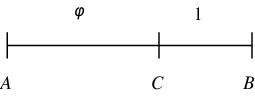
\includegraphics[scale=0.49,angle=0]{afsnit/baggrund/billeder/line_segment_a_c_b}
	\end{center}
	\caption{Euklids opdeling af et linjestykke}
	\label{line_segment}
\end{figure}

Givet et linjestykke $A\ B$, hvor $A\ B$ definerer linjen mellem
punkterne $A$ og $B$, som vist i figur \ref{euclid}, og ud fra Euklids
beskrivelse kan $\varphi$ defineres som
\begin{equation}
	\varphi	= \frac{A\ C}{C\ B} = \frac{A\ B}{A\ C}
	\label{euclid}
\end{equation}
Ved at indsætte variable i ligning \ref{euclid} får vi
\begin{equation}
	\varphi = \frac{\varphi + 1}{\varphi}
	\label{expand_euclid}
\end{equation}
hvilket giver os andengradsligningen
\begin{equation}
	\varphi^{2} - \varphi - 1 = 0.
	\label{poly_phi}
\end{equation}
Hvis vi nu løser andengradsligningen i \ref{poly_phi}, med
$\varphi > 0$, får vi
\begin{eqnarray*}
	\varphi	& =	& \frac{\sqrt{5} + 1}{2} \\
		& =	& 1.6180\ 3398\ 8749\ 8948\ 4820 \dots
\end{eqnarray*}

Tallet $\varphi$ bemærker sig blandt andet ved, at når det kvadreres, så
lægger man blot 1 til. Dette udledes trivielt fra ligning \ref{poly_phi}
\begin{equation}
	\varphi^{2} = \varphi + 1
	\label{phi_squared}
\end{equation}

Vi kan også finde polynomiets anden rod som angives ved $\varPhi$
\begin{eqnarray*}
	\varPhi & = & \frac{1}{\varphi} \\
		& = & \varphi - 1 \\
		& = & 0.6180\ 3398\ 8749\ 8948\ 4820 \dots
\end{eqnarray*}
Også tallet $\varPhi$ er interessant idet dets eget kvadrat plus sig
selv giver 1. Vi har at
\begin{equation}
	\varPhi^{2} + \varPhi = 1
	\label{Phi_squared}
\end{equation}
hvilket kun er gældende for $\varPhi$.

Tallet $\varphi$ fremviser endvidere en interessant forbindelse til
Fibonaccis talrække, da forholdet mellem to fibonaccital $F(n)$ og $F(n
- 1)$ konvergerer mod $\varphi$, når $n$ nærmer sig uendelig. Formelt har
vi at
\begin{eqnarray*}
	\varphi & =     & \lim_{n \rightarrow\infty}{\frac{F(n)}{F(n - 1)}}
\end{eqnarray*}

I tabel \ref{fibonacci_sequence} ses hvordan ratioen mellem fibonaccital
konvergerer mod $\varphi$, hvor også den procentvise afvigelse fra
$\varphi$ vises.

\begin{table}[h!]
    \centering
    \begin{tabular}{|c|c|c|c|c|}
        \hline
        $n$ & $F(n)$ & $F(n - 1)$ & $ \frac{F(n)}{F(n - 1)}$ & $\%$ fra $\varphi$ \\
        \hline
        0	 & 0 	 & $n/a$ & $n/a$ 		& $n/a$ 		\\
        1	 & 1	 & 1	 & 1.0		 	& 38.196601125 		\\
        2	 & 1	 & 1	 & 1.0		 	& 38.196601125 		\\
        3	 & 2	 & 1	 & 2.0		 	& -23.60679775 		\\
        4	 & 3	 & 2	 & 1.5			& 7.29490168752 	\\
        5	 & 5	 & 3	 & 1.66666666667	& -3.00566479165 	\\
        6	 & 8	 & 5	 & 1.6			& 1.11456180002 	\\
        7	 & 13	 & 8	 & 1.625	 	& -0.430523171858 	\\
        8	 & 21	 & 13	 & 1.61538461538	& 0.163740278863 	\\
        9	 & 34	 & 21	 & 1.61904761905	& -0.062645797602 	\\
        10	 & 55	 & 34	 & 1.61764705882	& 0.0239135845758 	\\
        11	 & 89	 & 55	 & 1.61818181818	& -0.00913636134662 	\\
        12	 & 144	 & 89	 & 1.61797752809	& 0.00348946069118 	\\
        13	 & 233	 & 144	 & 1.61805555556	& -0.00133290189271 	\\
        \hline
    \end{tabular}
    \caption{Fibonaccisekvens}
    \label{fibonacci_sequence}
\end{table}

\subsection{Et gyldent rektangel}
På samme måde som vi kan opdele et linjestykke efter det gyldne snit,
kan vi konstruere et rektangel, hvor forholdene mellem højde og bredde er
$\varphi$. Vi konstruerer et rektangel, hvor alle sider er lig 1, og
tegner en diagonal fra dette rektangels midte til dets modsatte hjørne. Med
denne diagonal som radius tegnes en cirkel, som et gyldent rektangel kan
tegnes efter. Figur \ref{golden_rectangle} illustrerer denne metode.

\begin{figure}[h!]
	\begin{center}
		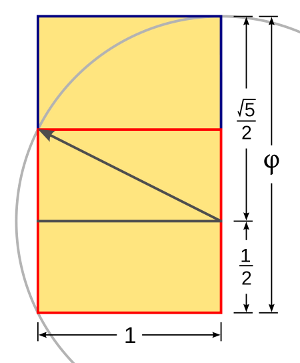
\includegraphics[scale=0.35,angle=0]{afsnit/baggrund/billeder/Golden_Rectangle_Construction}
	\end{center}
	\caption[Et gyldent rektangel]{Et gyldent rektangel - \emph{Kilde: Wikipedia}}
	\label{golden_rectangle}
\end{figure}
Det ses, at rektanglet har forholdet $\varphi:1$ og at eksemplet er helt
analogt til linjestykket givet i figur \ref{line_segment}. Dog skal
det bemærkes, at det rektangel, der kan konstrueres af linjestykkerne 1
og $\varphi - 1$, også er et gyldent rektangel med forholdet $1:\varphi
-1 = \varPhi$. Man kan derved konstruere gyldne rektangler ud i det
uendelige ved hele tiden at lave nye gyldne rektangler.

\subsection{Spiraler og det gyldne snit}
Når man, som ovenfor, gentagne gange deler et gyldent rektangel, kan man
bruge dette til at konstruere en gylden spiral. En gylden spiral kan
skrives ved ligningen for generelle logaritmiske spiraler som
\begin{equation}
	r = ae^{c\theta}
	\label{log_spiral_2}
\end{equation}
eller
\begin{equation}
	\theta = \frac{1}{c}\ln(r/a)
	\label{log_spiral_1}
\end{equation}
hvor $e$ er grundtallet for den naturlige logaritme og $c$ skal have en
speciel værdi for at kunne være en gylden spiral.

Det kan være svært at tegne logaritmiske spiraler korrekt, men man kan
approksimere en spiral ved at sammensætte dele af cirkler. Man kan
således approksimere en gylden spiral ved at sammensætte kvarte cirkler.
Denne approksimation giver dog ikke en ægte gylden spiral, og faktisk kan
ingen sådanne approksimationer af sammensatte cirkler gengives ved en
matematisk ligning\cite{Sharp2002}. Det er i tabel
\ref{fibonacci_sequence} vist hvordan Fibonaccis talrække konvergerer
mod det gyldne snit. Vi kan også konstruere et approksimeret gyldent
rektangel ud fra fibonaccitallene, som vist i figur
\ref{fibonacci_rektangel}, ved sammensatte $F(n)$ x $F(n)$-rektangler.
\begin{figure}[h!]
	\begin{center}
		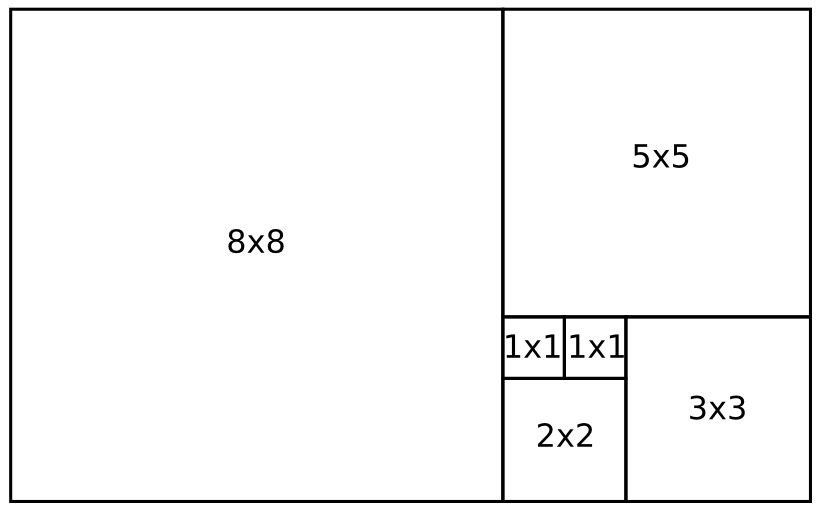
\includegraphics[scale=0.35,angle=0]{afsnit/baggrund/billeder/fib_rect}
	\end{center}
    \caption[Rektangel opbygget efter Fibonaccis talrække]{Rektangel
    opbygget efter Fibonaccis talrække. Man kan blive ved med at sætte
    $F(n)$ x $F(n)$-rektangler på denne figur og derved tilnærme sig et
    ægte gyldent rektangel jvf. tabel \ref{fibonacci_sequence}.}
	\label{fibonacci_rektangel}
\end{figure}
Vi kan nu tegne kvarte cirkler i figur \ref{fibonacci_rektangel}, med
radius $F(n)$, og derved approksimere en gylden spiral, som vist i figur
\ref{fibonacci_spiral}. Hvor tæt vi kommer på en egentlig gylden spiral
afhænger af, hvor mange rektangler vi har brugt til at tegne spiralen
efter. Et højere antal rektangler giver en spiral, som er tættere på en
egentlig gylden spiral. Formelt kan det direkte udledes af tabel
\ref{fibonacci_sequence}, hvor tæt en approksimation vi har på en gylden
spiral.
\begin{figure}[h!]
	\begin{center}
		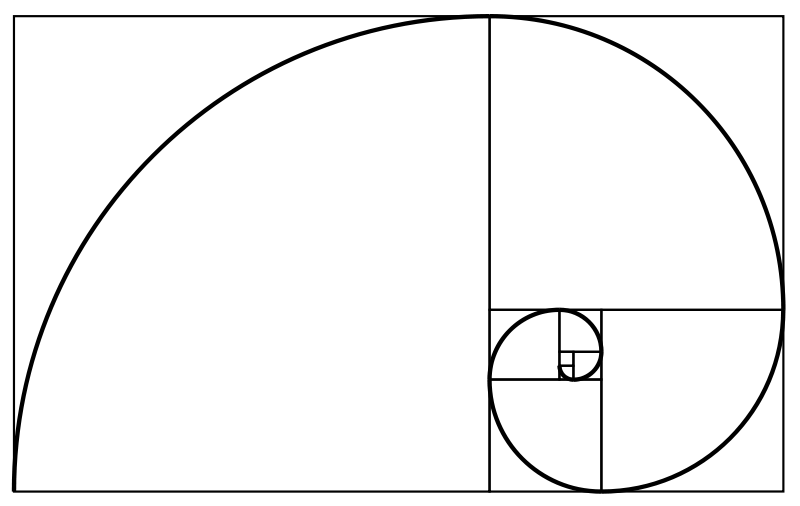
\includegraphics[scale=0.35,angle=0]{afsnit/baggrund/billeder/Fibonacci_spiral}
	\end{center}
	\caption[En fibonaccispiral]{En fibonaccispiral - \emph{Kilde: Wikipedia}}
	\label{fibonacci_spiral}
\end{figure}
Hvis man regner den korrekte faktor $c$ ud og tegner en ægte gylden
spiral i et gyldent rektangel vil man se at spiralen faktisk går
\emph{uden for} rektanglet\cite{Sharp2002}. Ovenstående approksimation,
med radius $F(n)$, vil aldrig gå ud over rektanglet, og det bliver derved
klart, at fibonaccispiralen i sandhed blot er en approksimation.

For en fuld gennemgang af spiraler, specielt med henblik på det gyldne
snit, se \cite{Sharp2002}. Vi vil nu kaste et hurtigt blik på
problematikken ved at afgøre hvad der er interessant i et billede og se
på hvordan computeren kan bruges i denne sammenhæng.

}
% vim: set tw=72 spell spelllang=da:


\section{Computeren som betragter\label{section_computer_betragter}}
{
Giver man tre forskellige mennesker den opgave at afgøre hvad der er det
interessante i et givet maleri, kan man meget vel få tre forskellige
svar. Mere kompliceret bliver det når man spørger ind til \emph{hvordan}
de er kommet frem til deres svar. Én begrunder måske sit valg med en
viden om netop det givne maleri, en anden med viden om maleriets
kunstner eller periode, mens en tredie begrunder det med æstetiske
virkemidler eller subjektive holdninger. Her er alle muligheder åbne for
at lave fejl, da man som regel ikke har kunstneren til rådighed til at
give det rigtige svar, hvis han da overhovedet selv kender det.
Maleriets motiv kan lede én på sporet af hvad der er interessant, men
dette kræver måske en viden om motivets bagvedliggende historie.
Mennesket tager altså en lang række overvejelser og baggrundsviden i
betragtning når ovenstående opgave skal løses.

Det interessante i et billede afhænger af den enkelte opgave.  Hvis vi
forestiller os en læge der kigger på et røntgenbillede af en patient som
har brækket armen, er det indlysende hvad lægen betragter som det
interessante i billedet, nemlig der hvor bruddet sidder. Når vi har med
tilfældige malerier at gøre, så står vi dog stadig tilbage med
spørgsmålet: \emph{``Hvad er egentlig \emph{interessant} i et maleri?''}
Vi lader dette spørgsmål stå åbent for at se på hvordan computeren
betragter et maleri.

\begin{figure}[h]
    \centering
    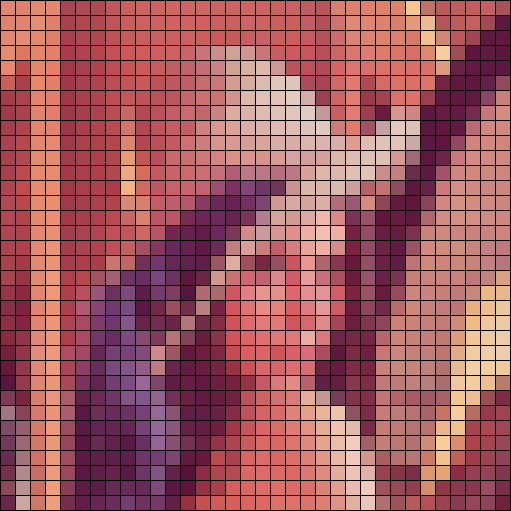
\includegraphics[scale=0.3]{afsnit/baggrund/billeder/pixel_lena}
    \caption[]{Pixels i et billede}
    \label{pixel_lena}
\end{figure}

Billedet i figur \ref{pixel_lena} er blevet delt op i nogle små felter
kaldet pixels. Hver pixel har en farve. Computeren opfatter et billede
netop som pixels. Computeren ser endvidere disse pixels \emph{én ad
gangen}. Det svarer altså til at den enkelte farve til en pixel bliver
læst op for en person der ikke kan se selve billedet. For at køre
eksemplet helt ud, så har vi at en person får følgende at vide:
\begin{quote}
    \emph{``Pixel med koordinater $(0, 0)$ er gul. Pixel med
    koordinater $(1, 0)$ er orange''} etc.
\end{quote}
Dette giver ingen egentlig information om \emph{hvad} billedet
forestiller. Computeren kan ikke se billedet i sin helhed og har som
udgangspunkt ikke nogen baggrundsviden at basere en vurdering på. Det
eneste computeren kan gøre er at gå billedet igennem pixel for pixel og
sammenligne dem.

Vi ønsker at bruge computeren til at afgøre om der ligger noget
interessant i billedet omkring det gyldne snit. Vi vil derfor nu kaste
et blik på den forskning der allerede er blevet gjort på dette område.

}

% vim: set tw=72 spell spelllang=da:


\section{Eksisterende forskning\label{section_forskning}}
{
Som allerede nævnt, kendte de gamle grækere til tallet $\varphi$, som
Euklid kaldte for \emph{the division in extreme and mean ratios},
forkortet DEMR. Luca Pacioli udgiver i 1509 bogen \emph{De divina
proportione}, som beskriver samme fænomen omtalt som ``den guddommelige
propertion''. Udtrykket ``det gyldne snit'' kan spores tilbage til
tyskeren Martin Ohm (1792 -- 1872), der første gang betegner Euklids DEMR
som \emph{der Goldener Schnitt} i sin bog \emph{Die reine
Elementar-Mathematik}, fra 1835\cite{Markowsky1992}. Det gyldne snit er
nu blevet den foretrukne betegnelse.

Nu bliver det påstået, fra flere kilder, at det gyldne snit bruges i
malerier, arkitektur og musik, da dette forhold har specielt tiltalende
æstetiske
egenskaber\cite{GoldenNumber,RatioArt,Putz1995,Stakhov2006490,Boussora2004}.
Især \cite{GoldenNumber} er særlig ivrig og finder det gyldne snit i alt
lige fra cigaretpakker til skallen fra en nautil. Netop nautilskallen
bliver meget ofte brugt som argument for, at det gyldne snit findes i
naturen i form af en gylden spiral lignende den fra figur
\ref{fibonacci_spiral}. Hvis man rent faktisk måler efter,
viser det sig, at dette ikke er tilfældet. Som argumenteret i
\cite{Sharp2002} er spiralen i nautilskallen rigtigt nok logaritmisk,
men ikke med en faktor $c$ som ville gøre den til en gylden spiral.

Det græske tempel Parthenon spiller også en central rolle i påstanden om
det gyldne snit. Billeder af templet bliver tit vist med et rektangel
tegnet over. Der florerer forskellige udgaver af disse billeder, hvor
der åbenbart ikke tages højde for, at dele af templet ikke indgår i
rektanglet eller fotografiets perspektiv. George Markowsky gør i
\cite{Markowsky1992} op med mange af disse vrangforestillinger. Påstande
om, at Keopspyramiden skulle være bygget efter det gyldne snit --- som
angivet i \cite{Stakhov2006490} --- at nogle af Leonardo da Vincis malerier
er malet efter det gyldne snit, og at det gyldne rektangel er det mest
æstetisk tiltrækkende format\cite{GoldenNumber,RatioArt}, bliver i
hans artikel afvist, da mange af disse undersøgelser lider under det, han
kalder \emph{the Pyramidology Fallacy}. Dette udtrykt henter Markowsky
fra \cite{Gardner1952_2} og beskriver de personer, der forsker i
pseudovidenskab såsom pyramidernes arkitektur. Her har forskerne ofte
mange forskellige tal at ``jonglere'' med og kan frit vælge netop dem,
der giver det ønskede resultat. En anden forfatter, Roger
Hertz-Fischler, er ligeledes optaget af den specielle værdi, det gyldne
snit er blevet tillagt. Det som Markowsky og Gardner kalder for
\emph{Pyramidology}, betegner han som \emph{golden numberism}, og han har
fulgt dette fænomens historie tilbage til en tysk mand ved navn
Adolph Zeising (1810 -- 1876)\cite{Herz-Fischler2005}. Hertz-Fischler
hævder, at stort set alle undersøgelser inden for \emph{golden numberism}
kan spores tilbage til Zeising.

Hypotesen om det gyldne rektangels æstetiske egenskaber bliver også
taget op i \cite{Boselie1984} og \cite{Plug1980}, hvor det ikke kan
konkluderes, at det gyldne rektangel skulle have nogen æstetisk
signifikans. En lignende hypotese bliver sat på prøve i
\cite{McManus1995}, hvor det undersøges, om et billedes geometriske
komposition har indflydelse på dets æstetiske effekt. I. C. McManus
kunne, gennem tre eksperimenter, ikke finde noget grundlag for, at et
billedes geometriske komposition, påvirkede testpersonernes bedømmelse.
Det siges i konklusionen:

\begin{quote}
	\emph{``Together the results of these experiments throw
	considerable doubt upon the hypothesis of the implicit detection
	of latent compositional geometry as a major component of
	aesthetic judgements, at least for relatively unsophisticated
	observers[\dots]''}
\end{quote}

Selvom ovenstående ikke eksplicit nævner det gyldne snit, har det
alligevel en klar relevans til billeder opbygget geometrisk efter det
gyldne snit.

Der ses dog et klart problem, hvilket Markowsky også nævner, idet det
ikke er defineret, hvornår et stykke kunst er konstrueret efter det
gyldne snit. Ej heller er det defineret, præcis hvordan man finder det
gyldne snit: Der findes mange billeder, hvor snittet er illustreret vha.
linjer, men størstedelen af disse har ikke de fornødne mål, og det
gyldne snit findes gerne helt arbitrære steder uden nogen som helst
identificerbar fremgangsmåde.  Én undersøgelse, omhandlende billeders
komposition, har dog lavet statistik på 565 malerier, men kun forholdet
mellem lærredets dimensioner er blevet registreret\cite{Olariu1999}.
Denne undersøgelse kunne ikke konkludere, at kunstnere foretrækker det
gyldne snit i lærredet.

Det er derfor interessant at forsøge at automatisere søgningen efter det
gyldne snit i malerier og fastsætte klare kriterier for, hvornår et
malerier indeholder objekter, som ligger i det gyldne snit.  Til denne
opgave er det oplagt at udnytte regnekraften fra computeren, for at
sikre en ensartet bedømmelse af malerierne.

\subsection{Eksisterende datalogisk forskning}
Tidligere datalogiske forskning indenfor detektion af det gyldne snit er
ikke eksisterende. Derfor bliver vi nød til at kigge på generelle teorier og algoritmer
indenfor billedbehandling, mest i retning af  analyse af interessante
regioner. Den mest relaterede forskning er et eksperiment, som
analyserer æstetik i fotografier\cite{DattaWang}.
Det væsenlige ved dette eksperiment er hvorledes billederne
bedømmes. Her arbejdes der med 56 forskellige kandidater til at definere
et billede, som er mere eller mindre æstetisk korrekt og originalt. 
Kandidaterne bliver udvalgt i forskellige kategorier, tre af
kandidaterne bliver vurderet ud fra ``The rule of Thirds'', som er 
beskrevet således.
\begin{quote}
	``The rule can be considered as a sloppy approxmination of the
	golden ratio (about 0.618)''
\end{quote}

%fyld? Meget fedt at få sagt det men jeg ved ikke om det er specielt
%vigtigt
Denne artikels kandidater dækker over noget ganske centralt i
billedbehandling nemlig detektion af
interessante regioner i billeder, problemet er at begrebet slet ikke er
entydigt defineret, men skifter betydning fra fagområde til fagområde.
Hvad vi opfatter som interessant vil blive diskuteret i \ref{section_kort_intro}

Den første er maskineindlæring, der stammer fra feltet kunstig
intelligens indenfor datalogi. I billedbehandling bliver det dog
brugt til at finde interessante regioner med stor præcision, og formålet
med brugen er blandt andet at finde ansigter, mennesker og
biler\cite{ViolaJones01,SchneidermanKanade00,Gabor}. Præcisionen på
algoritmernes detektion betyder dog en øget kompleksitet i udvikligen. 

Den anden er opdelinger af billeder efter tekstur. Ideen bag denne type
af metoder er at opdele efter
overfladetekstur\cite{218442,CarsonBelongie02,PapageorgiouPoggio}.
Der er mange forskellige algoritmer, der arbejder på så forskellige ting
som farveklatter og detektion af mønstre\cite{PalPal}.

}
% vim: set tw=72 spell spelllang=da:


\section*{Opsummering}
Den matematiske definition, giver os nogle værktøjer, til at analysere
malerier for brug af det gyldne snit.  Den eksisterende forskning, eller
mangel på samme, fortæller os, at det er en meget svær opgave, at bruge
computeren til at fortolke malerier, og at det er tvivlsomt, hvorvidt
det gyldne snit kan tillægges nogen speciel værdi.  I næste afsnit vil
vi se på, hvilke metoder vi vil bruge, for at undersøge det gyldne snit
i digitale gengivelser af malerier.

}

% vim: set tw=72 spell spelllang=da:


\chapter{Detektion af det gyldne snit\label{chap_detektion}}
\subsection{Opdeling af billeder}
\textsf{
Mange af de metoder, vi bruger til at udregne, det gyldne snits position
eller størrelsen af en margin, udregnes med brøker. Hvorimod et billede
opbygges af pixels. Dette gør, at vi bliver nødt til at tage
approksimationer af udregningerne. Vi vil også kommer ind på nogle af de
fejl som kan opstå i tilblivelse af maleriet}

\subsection{Inddeling af billede efter snit}
Vi vil i dette afsnit give nogle definitioner på hvordan et billedet er
bygget op, samt hvilke afrundings fejl der kan opstår ved denne
opbygning. For at få nogle faste definitioner på hvordan et billedet ser
ud samt hvad et snit er, har vi stillet de her to definitioner op.

\begin{definition}
	I et billede betegnes \textbf{højden og bredden} som hhv. $H$ og
	$B$, som illustreres i figur \ref{cut}.
\end{definition}

\begin{definition}
	Et \textbf{snit} er en lige vertikale eller horisont linje, som
	strækker sig fra kant til kant.
\end{definition}

\begin{figure}[h]
	\begin{center}
		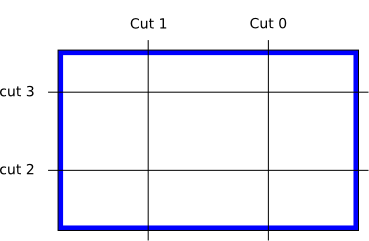
\includegraphics[scale=0.42,angle=0]{afsnit/vores_implementation/billeder/naiv_algoritme/Cut}
	\end{center}
	\caption[]{Billedets højde og bredde betegnes hvv. H og B. De 4 snit er navngivet.}
	\label{cut}
\end{figure}

End til vider har vi kun arbejder med det gyldne snit, men andre snit i
billedet kan godt optræde, derfor indføre vi en nu betegnelse
snitratio.

\begin{definition}
	En \textbf{snitratio} er en procents sats, som ganget på $B$ eller
	$H$, finde placeringen af et snit i billedet.
\end{definition}

Det vil sige at hvis en snitration er på $0.2$. Et billedet har $B$ på
4000 vil et snit befinde sig i pixel $4000*0.2 = 800$ fra højre side af
billedet, det samme antal pixel fra venstre side vil også være et snit.
Samme metode kan bruges på $H$ for at få 2 snit mere. 

\begin{definition}
	For vær snitration er der fire snit, to i det vertikale plan og to i
	det horisontale plan, som er illustreret på maleri \ref{lenasnit2},
	med røde streger. Med mindre snitration er 0.5, så er der kun 2 snit.
\end{definition}

Hvis snitratioen er $0.5$ kommer snittene til at ligge over på hinanden,
og derved vil snitratioen kun have 2 snit, de 2 snit Id, samt snitenes
plascring kan ses i figur \ref{2Cut}.

\begin{figure}[h]
	\begin{center}
		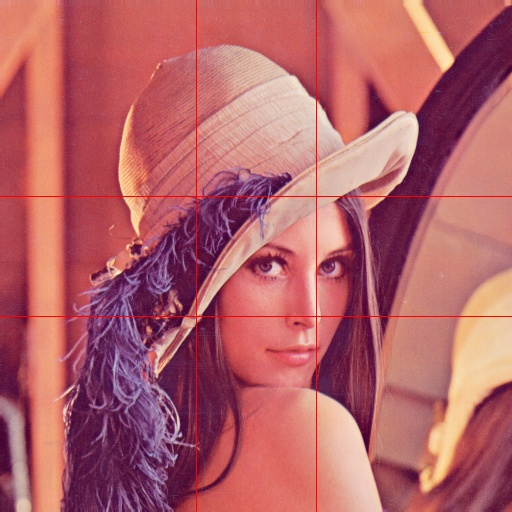
\includegraphics[scale=0.42,angle=0]{afsnit/vores_implementation/billeder/naiv_algoritme/Lenagolden}
	\end{center}
	\caption[]{Billedet som har indtegnet de fire gyldne snit}
	\label{lenasnit2}
\end{figure}

De 4 snit tildeles hvert deres Id, "snit 0,1,2 og 3" så vi kan kende
forskel på de individuelde snit, Id'erne placering kan ses i figur
\ref{cut}. Vi vil i resten af rapporten kalde snittene efter deres Id.

\begin{definition}
	Vær snit af vær snitratio, har et fast \textbf{Id}, "Snit 0,1,2 og 3", som kan ses i figur \ref{cut}, hvor vært snit er indtegnet, samt deres Id som label. 
\end{definition}

\begin{figure}[h]
	\begin{center}
		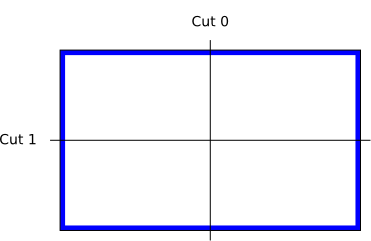
\includegraphics[scale=0.42,angle=0]{afsnit/vores_implementation/billeder/naiv_algoritme/2Cut}
	\end{center}
	\caption[]{Billedet skæres her kun af 2 snit}
	\label{2Cut}
\end{figure}

\subsection{Acceptabel afvigelse}
\begin{comment}"""
Som beskravet i afsnit \ref{mange_tal}, udregnes det gyldne snit med mange decimaler. Selv den beste kunstner har et maksimum på hvor præcis han kan male, om det er hans øjne der sætter grandsen eller størrelsen på han pensler eller om han bare ikke maler særlige præcis, så kan han aldrig malle så præcis som vi kan udregne det gyldne snit til. Derfor sætter vi en afvigelse på $0.5 \%$, som maleren vi sat en 
\end{comment}
\note{Nogle referanse}Som beskrevet i afsnit \ref{mange_tal}, udregnes
det gyldne snit med mange decimaler. En kunstner, hvor god han end er,
har ingen chance for at male så præcist at man kan sige at strøget
ligger nøjagtigt oven på snittet selv om hans intentioner er at ramme
snittet. Vi kommer derfor til at have en vis uprecis hed på de data vi
få fra billedet selv. Vi starter med at se på alle de ting, som kan
skabe en usikkerhed fra malerens side. Man kan gå ud fra at den
procentvise afvigelse ikke er særlig stor, da vi ikke har bestræbelser
på at arbejde på abstrakt malerier, dog har vi sat den procentvise
afvigelse til 0.5 \%. Det vil sige at en maler med et lærred på 100
cm, maksimalt vil male $0.5$ cm forkert.

Når maleren vælger en ramme og et lærred, har vi igen problematikken,
selv om maleren spicifikt gå efter at bygge maleriet op efter det gyldne
snit, kan snittets placering i maleriet have forskubbet sig, ved dårlige
valg at ramme eller lærred. Derfor sætter vi den afvigelse til $1\%$. Da
vi igen mener at dette er den maksimale afvigelse, der kan opstå.

Når maleren maler en region i et maleri, forekommerer der normalt en
lille kant rundt om objektet, et omrids. Dette omrids kan vores
algoritmer ikke tage højde for, og vi må derfor modregne omridset, så vi
er sikre på at vi ser på regionen og ikke dens omrids. Da et omrids ikke
er særligt stort, har vi sat denne procentsats til $0.5\%$. 

Alt i alt giver det en afvigelse på vores aktuelle udtrækning af data
fra malerierne på $2\%$ det vil sige at finder vi en region, som ligger
på pixel 200, i et billedet, der er $500$ cm bredt, befinder den sig
faktisk i intervallet [190,210]. Måden hvorpå vi tager højde for den
forskel, er ved hjælp af marginer, som nævnt i afsnit
\ref{section_naiv}.


\subsection{Heltal i det gyldne snit}
Nå vi udregner hvor et snit for et billedet med $H = 4000$,
approksimerer vi antal pixels ved at afrunde resultatet $2472.13595
\approx 2472$, se udregning \ref{afrundning}. Det betyder at vi mister
0.13595 pixels i præction, hvilket svarer til en misvisning af punktet
på 0.00339875 $\%$ i forholdt til $B$ på billedet. Se udregning
\ref{afrundning2}.

\begin{equation}
	4000 \cdot \varPhi = 4000(\sqrt{5}-1)/2 = 2472.13595 \approx 2472 \label{afrundning}
\end{equation}

\begin{equation}
	0.13595/4000 \cdot 100 = 0.00339875 \label{afrundning2}
\end{equation}

Det er en meget lille del af selve billedet og skulle ikke give nogle
misvisninger i forhold til udregningen. For at gøre det lidt mere
generelt, sætter vi trunkeringsfejlen til $0.5$, da det er den maksimale
afrundingsfacktor som kan forekomme. Hvis billedet har en størrelse på
500 pixels, hvilket er det mindste billedet vi har, giver dette en fejlmargin
på $0.1 \%$. Dette tal bliver adderet til fejlsatsen ovenfor, og giver
en samlet afvigelse på $2.1\%$.



\subsection{Heltal ved udregning af Margin}
Når vi har 2 forskellige snitratioer, f.eks. $\varPhi$ og $\frac{2}{3}$,
som ligger meget tæt på hinanden, og vi gerne vil sammenligne hvilken
regioner der ligger i snitratioernens snit, er det vigtigt at margin for
vært af de 2 snitratioers snit ikke krydser hinanden. 

Hvis margin krydser. Vil det indebære, at den samme region bliver fundet
af begge snit. Dette vil give et skævt billedet af forskellen på de to.
Derfor må vi sørge for at marginerne ikke krydser. Hvis $x$ betegner
antal pixels i $B$ eller $H$, og vi vil se på, hvor mange pixels, der er
mellem snitratio $\frac{2}{3}$ og $\varPhi$, multiplicerer vi $x$ med de
to snitratioen for at finde deres placering. Derefter subtraheres vi et
af de snit som befinder sig tetest på hinanden i vær snitratio med
hinanden.


\begin{eqnarray}
	\frac{x2}{3} - \frac{x2}{\sqrt{5}+1} & = & x(\frac{2}{3} - \frac{2}{\sqrt{5} + 1}) \nonumber \\
	& = & x(0.666667-0.618034) \\ \nonumber
	& = & x(0.048633)
\end{eqnarray}

Vi har nu fundet antal pixel mellem de to snit. Vi vil gerne undgå at
de to marginer krydser hinanden, så vi dividere antal pixel mellem de to snit med to og afrunder værdien.

\begin{equation}
	\left\lfloor \frac{0.048633x}{2}\right\rfloor = \left\lfloor0.024316x \right\rfloor
	\label{marginstoerlse}
\end{equation}

Den minimale procentvise størrelse, margin må have, når vi
sammenligner det gyldne snit og $\frac{2}{3}$, er altså $2.4316$ Det
betyder også, at vi ikke må sammenligne snit som ligger særlig meget
tætter på hinanden, da $2.1\%$ er den minimale procent margin som vi må
have. For at vise, hvor stor marginen egentlige kan være, bruger vi formel \ref{marginstoerlse} på to billeder, et, som svarer til vores mindste billede, på
500 pixels, og et, som svarer til vores største billede, på 4000 pixels. Ved
500 pixels bliver resultatet.

\begin{definition}
	Margins størrelse i et snit, må ikke overstige $2.4316 \%$, af det respektive maleri $B$ eller $H$.
	\label{margin_max}
\end{definition}

\begin{definition}
	Margins størrelse i et snit, må ikke kommer under $2.1 \%$, af det respektice maleri $B$ eller $H$.
	\label{margin_min}
\end{definition}

\note{Er det denne måde det skal stilles op?}
\begin{equation}
	 \lfloor 500(0.024316)\rfloor = 12
\end{equation}

Det er en fin margin, da vores fejl på udregningerne ligger på 2.1 \%,
som svarer til $\lceil 500*0.021 \rceil = 11$ pixels. Der er 1 pixel fra vores
margin.

Ved 4000 pixels giver det.

\begin{equation}
	 \left\lfloor 4000(0.024316)\right\rfloor = 97
\end{equation}

Som også er god nok, da $4000*0.021 = 84$ pixels.
% vim: set tw=72 spell spelllang=da:

\subsection{Database}
{
Når vi har trukket regioner ud af billedet og vurderet dem efter
ovenstående simple algoritme kan vi stå tilbage med et egentligt
resultat. Vi ønsker at gemme dette resultat i en database så vi på et
senere tidspunkt kan bruge det i en samlet analyse af resultaterne.
Vi så i afsnit \ref{section_opbv_billeder} på et databaseskema til
opbevaring af maleriers metadata. Vi bygger nu videre på dette skema så
vi kan tilknytte resultater fra en analyse til de enkelte malerier. Det
fulde databaseskema ses nedenfor.

\begin{table}[!h]
    \centering
    \begin{tabular}{|l||c|c|c|c|c|c|}
        \hline
        \bf{artist} \hspace{0.5cm} & \underline{artistId} & name & born & died & school & timeline \\\hline
    \end{tabular}
    \caption{Databasetabel for kunstner}
    \label{artistTable}
\end{table}

\begin{table}[!h]
    \centering
    \begin{tabular}{|l||c|c|c|c|c|c}
        \hline
        \bf{painting} \hspace{0.5cm} & \underline{paintingId} & artistId & title & date & paint & $\cdots$ \\\hline
    \end{tabular}\\ \vspace{0.2cm}\hspace{1.2cm}
    \begin{tabular}{c|c|c|c|c|c|c}
        \hline
        $\cdots$ & material & location & url & form & type & $\cdots$ \\\hline
    \end{tabular}\\ \vspace{0.2cm}\hspace{1.4cm}
    \begin{tabular}{c|c|c|c|c|c|}
        \hline
        $\cdots$ & realHeight & realWidth & height & width & filepath \\\hline
    \end{tabular}
    \caption{Databasetabel for malerier}
    \label{paintingTable}
\end{table}

\begin{table}[!h]
    \centering
    \begin{tabular}{|l||c|c|c|c|c|c|c|}
        \hline
        \bf{run} \hspace{0.5cm} & \underline{runId} & trsh1 & trsh2 & lo & up & marginPercentage & method \\\hline
    \end{tabular}
    \caption{Databasetabel for en kørsel}
    \label{runTable}
\end{table}

\begin{table}[!h]
    \centering
    \begin{tabular}{|l||c|c|c|c|c|c|}
        \hline
        \bf{result} \hspace{0.5cm} & \underline{resultId} & runId & paintingId & cutRatio & cutNo & numberOfRegions \\\hline
    \end{tabular}
    \caption{Databasetabel for resultater}
    \label{resultTable}
\end{table}

\begin{table}[!h]
    \centering
    \begin{tabular}{|l||c|c|c|c|c|c|c|}
        \hline
        \bf{region} \hspace{0.5cm} & \underline{regionId} & resultId & x & y & height & width & area \\\hline
    \end{tabular}
    \caption{Databasetabel for regioner}
    \label{regionTable}
\end{table}

Tabellerne \ref{artistTable} og \ref{paintingTable} er de samme som vist
i afsnit \ref{section_opbv_billeder}, men er taget med her blot for at
vise databaseskemaet i sin helhed. Det øvrige databaseskema lægger vægt
på at minimere redundans og mulighed for at genskabe kørte analyser.
Sidstnævnte er vigtig osv\dots

}
% vim: set tw=72 spell spelllang=da:



\chapter{Afprøvning\label{chap_afproevning}}
{
I dette Kapitel vil vi afprøve vores 2 metoder på XX(hvormange) billeder og se hvordan de virker. Udover det vil vi finde tærskelværdier til kandetection, floodfill og margin, ud fra observationer gjort under afprøvning. Vi vil også afprøve den generalle region detektor og kommer ind på dens fordele og ulemper. 
\section{Tærskelværdier}
I vores program er der 3 forskellige tærskelværdier som påvirker hvordan
metoden analysere billedet. Marginens brede, afvigelsen af farven i
floodfill og afvigelsen i farven i kandtdetectionen. Alle 3 tærskelværdier er
blevet introduceret i deres respektive afsnit, men ingen konkrate tal
er opgivet. I dette afsnit vil vi opgive de tal, samt en forklaring på
hvorfor vi har valt lige de tal.

\subsection{Marginens brede}
Vi regner marginens brede, $MB$ ud fra en procent af billedets brede og
højde. I afsnittet \ref{opdeling_af_billeder.tex} kom vi frem til en
usikkerhed på $2.1 \%$. Så vores $MB$ skal mindst
være på $2.1 \%$. Ud over det er den minimale forskel på 2 snit vi foretager os,
forskellen mellem det gyldne snit og $\frac{2}{3}$, som vi udregnet i
sektion \ref{opdeling_af_billeder.tex} til maksimalt at have en $MB$ på
$2.43$, for at margin ikke krydser. Så $MB \in [2.1, 2.43]$. Vi har valt
at sætte $MB = 2.4$, da vi derved kan tage højde for uforresette
usikkerhed. XXX(er det en dog nok forklaring).

\subsection{Afvigelsen af farver i kandtdetection}
Det vi bruger kandtdetection til, er af finde en kanter rundt om de
regioner som vi mener er interessante, og undgå de kanter som ligger
inde i regioner. Begge de 2 mål kan ikke altid opfyldes, men vi kan
komme så tæt på et krompromi mellem en perfekt kant rund om region og
ingen kanter inde i region som mulige. Dette gøres ved at ændre 2
tærskelværdier i kantdetectionen ud for observationer som vi har taget
på billederne i forvejen. Vi har valt at dele billederne som vi
observere op i 9 kategorier, som kan ses i tabel
\ref{thressholdsTabelKant}, Kategorier er en grove opdeling af
billederne efter detaljer og farve intensitet, som bruges til at give en
bedre indblik på billedets opbygning. 

\subsubsection{Sammenligninger}
Vi har set på XX(hvor mange) antal malerier og har fundet de
tærskelværdier som vi mener passer bæst på billedet. Vi vil illustrerer
den fremgange måden vi har brugt til at finde tærskelværdierne på, på
maleriet \ref{kDetalier}. Maleriet er malet med mange farver og med
masser af detaljer. Vi ser først på tærskelværdierne
$[0,0],[100,100]......[900,900],[1000,1000]$ se figur \ref{allesammen1}
og \ref{allesammen2}, og finde det interval hvor malerriet ikke har
mistet nogle af kanterne rundt om regionerne i nu, men vil det, i næste
interval. I illustration vurdere vi det til billedet \ref{300-300}, da
billedet \ref{400-400} har mistet for mange af de kanter, som vi gerne
vil beholde. Så tærskelværdien som vi gerne vil finde frem til, befinder
sig fra $[300,300]$ og frem. Ved at sætte den anden tærskelværdig op
lidt af gangen kan vi igen få en række billeder at vælge imellem, for at
få det beste resultat, se sammenligningen i figur \ref{allesammen3}. som
man kan se begynder det er være svær at skelne figurene i \ref{300-850}
og der er lidt for mange kanter i \ref{300-700}, så vi har valt at bruge
tærskeværdigerne $[300,750]$ for dette billedet. Man kunne god gå længer
ned og se om tærskeværdig $[300,745]$ passet bedre, men vi har valt at
holde . Det maleri vi lige har brugt er ikke særlige repræsentativ for
helle vores maleri database, så vi har taget en række billeder og brugt
samme metode på dem og kommer frem til en middel tærskelværdi, jeg viser
her en lille udsnit af dem, se figur \ref{en}, \ref{to} og \ref{tre}.

\begin{figure}[p]
    \centering
    \subfloat[100,100]{
        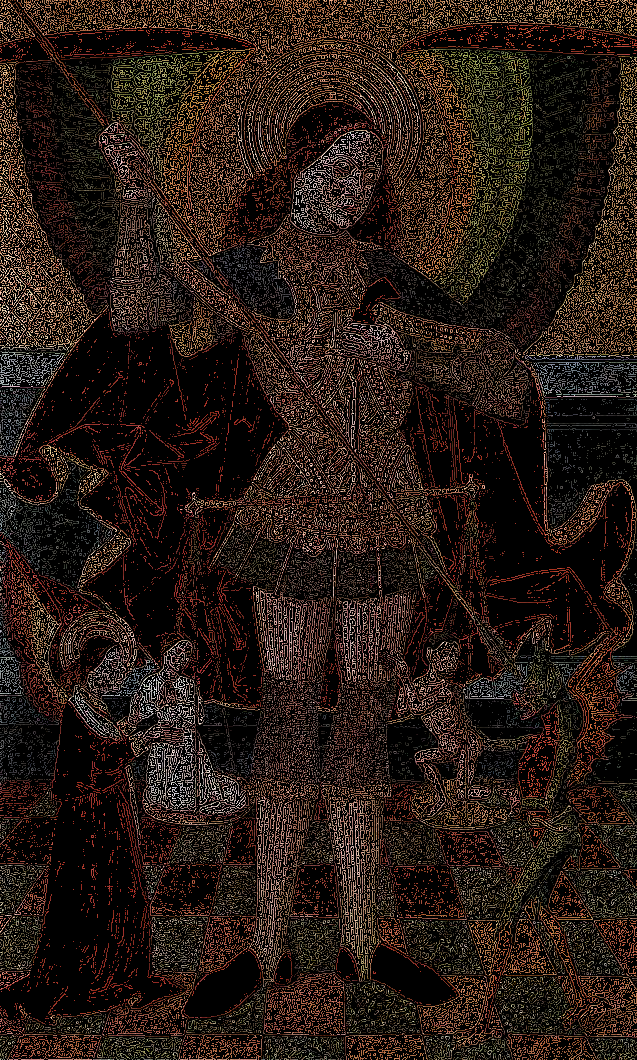
\includegraphics[angle=0,width=0.45\textwidth]{afsnit/afprovning/billeder/thressholds/krafitige_farver/krafite_detalier/1_iteration/100-100.png}
        \label{100-100}}\hspace{1em}
    \subfloat[200,200]{
        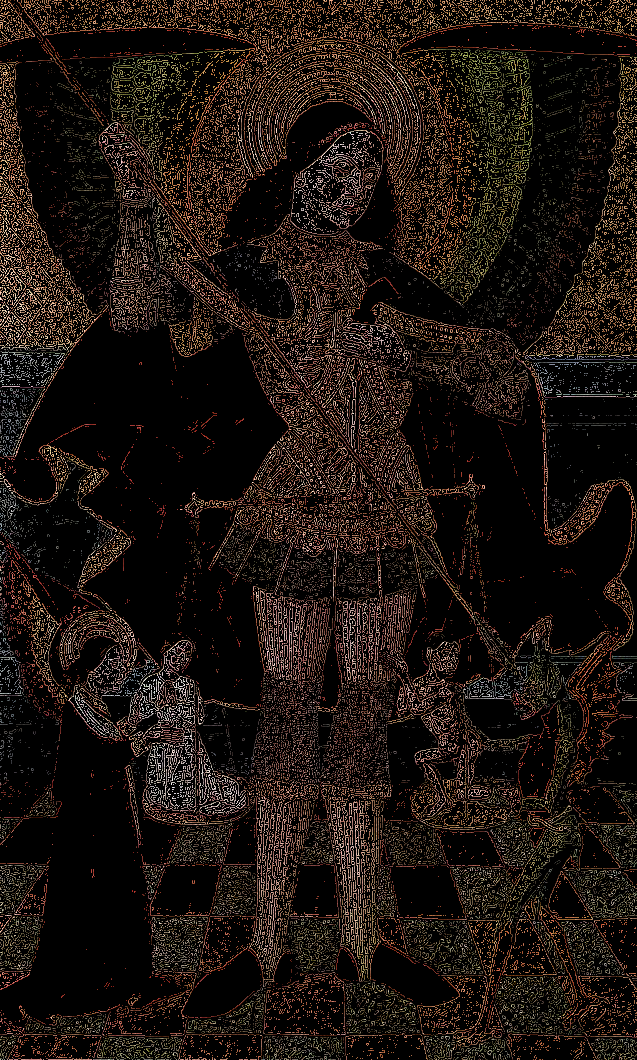
\includegraphics[angle=0,width=0.45\textwidth]{afsnit/afprovning/billeder/thressholds/krafitige_farver/krafite_detalier/1_iteration/200-200.png}
        \label{200-200}}\\
    \subfloat[300,300]{
        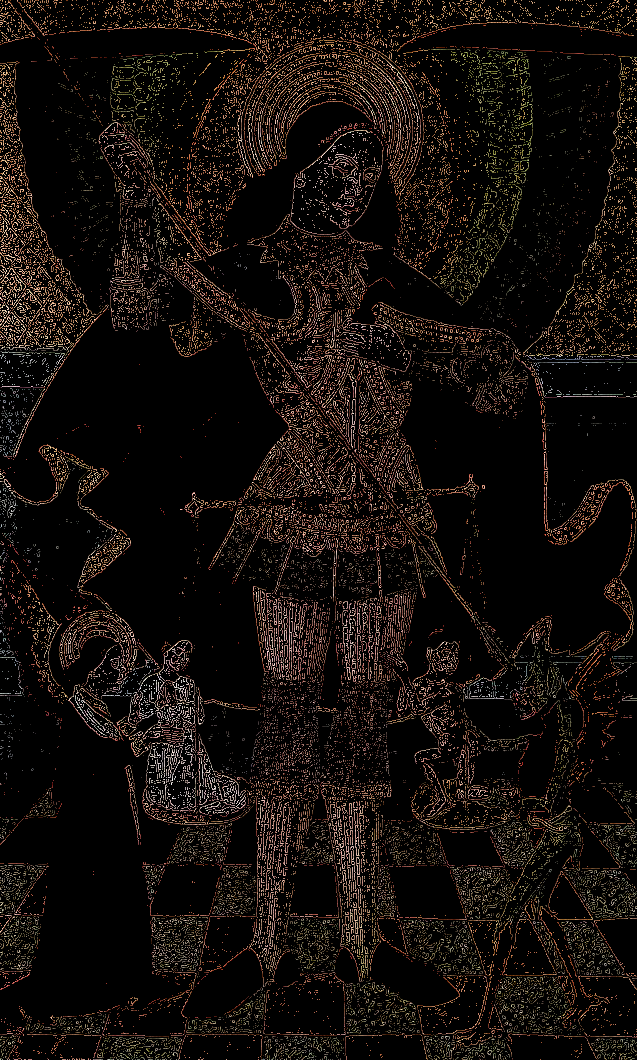
\includegraphics[angle=0,width=0.45\textwidth]{afsnit/afprovning/billeder/thressholds/krafitige_farver/krafite_detalier/1_iteration/300-300.png}
        \label{300-300}}\hspace{1em}
    \subfloat[400,400]{
        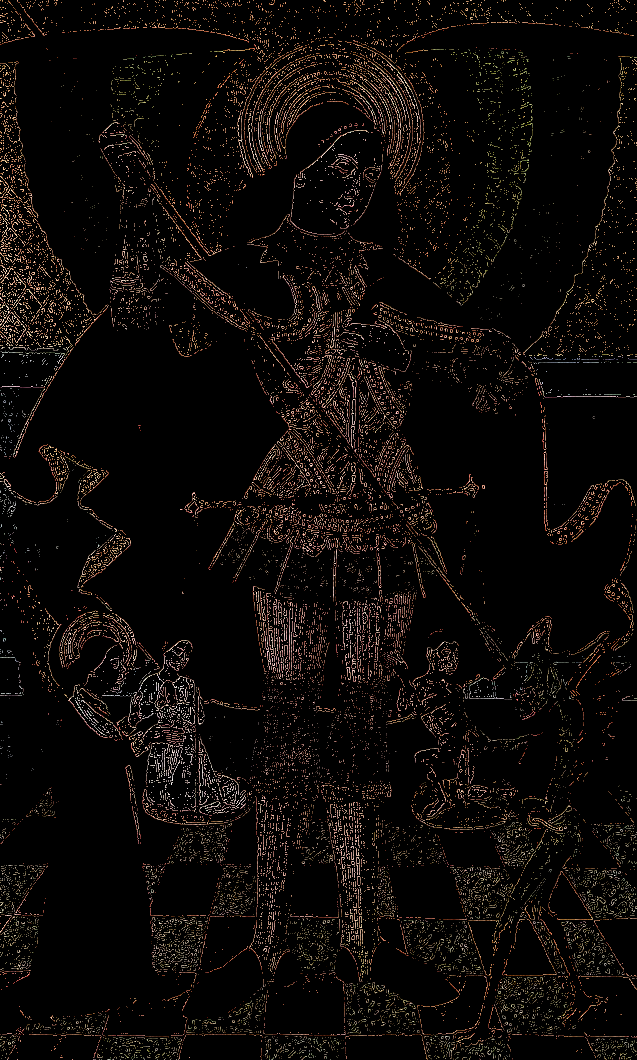
\includegraphics[angle=0,width=0.45\textwidth]{afsnit/afprovning/billeder/thressholds/krafitige_farver/krafite_detalier/1_iteration/400-400.png}
        \label{400-400}}
    \label{allesammen1}
    \caption{Hvad er et her?}
\end{figure}

\clearpage

\begin{figure}[!h]
	\centering
	\subfloat[500,500]{
        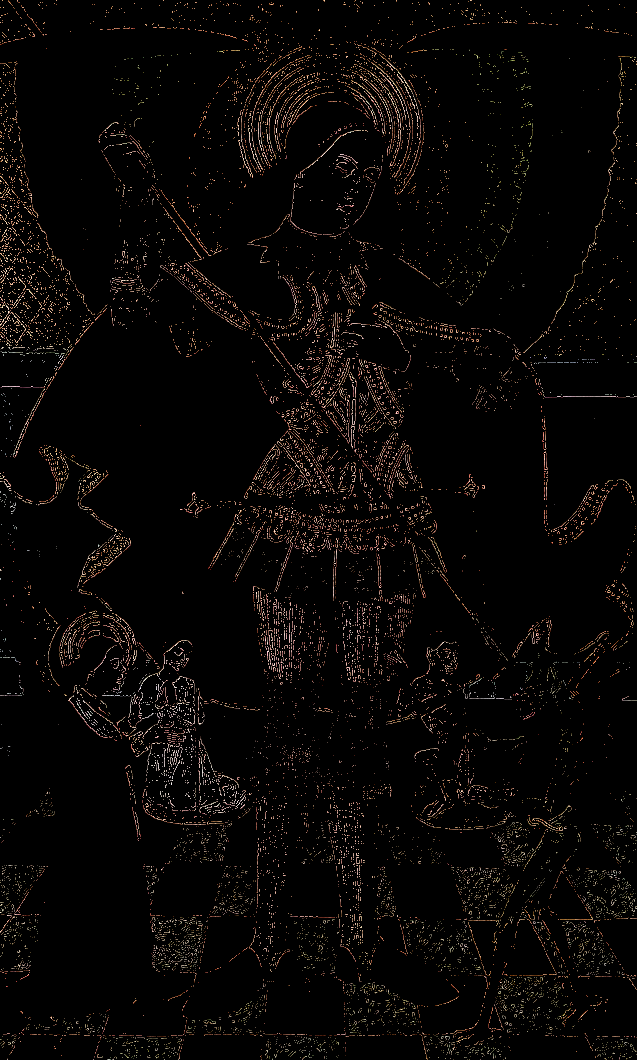
\includegraphics[angle=0,width=0.45\textwidth]{afsnit/afprovning/billeder/thressholds/krafitige_farver/krafite_detalier/1_iteration/500-500.png}
        \label{500-500}}\hspace{1em}
    \subfloat[600,600]{
        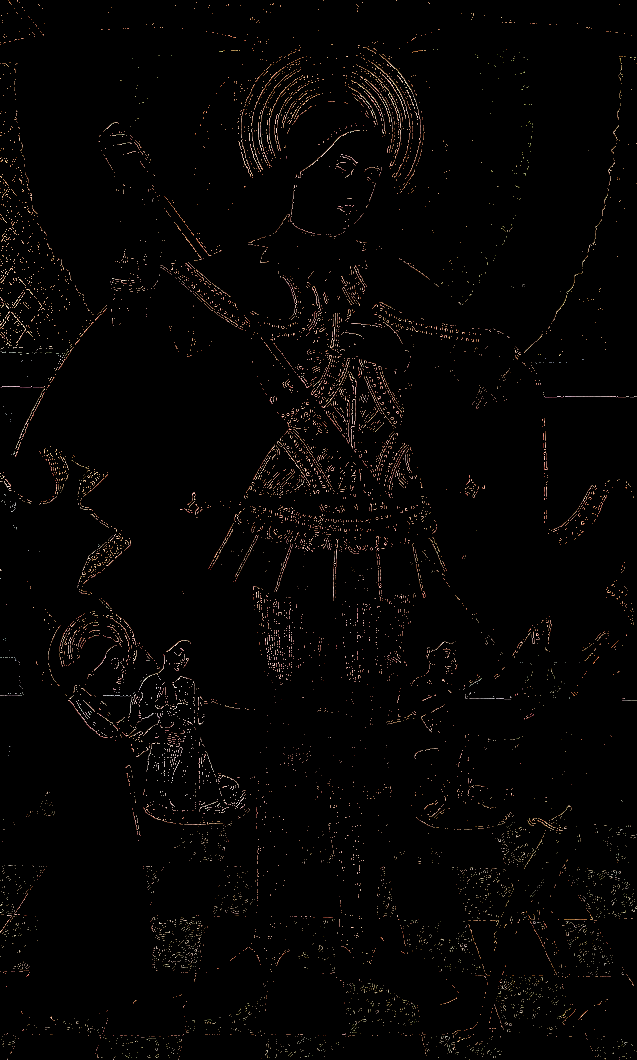
\includegraphics[angle=0,width=0.45\textwidth]{afsnit/afprovning/billeder/thressholds/krafitige_farver/krafite_detalier/1_iteration/600-600.png}
        \label{600-600}}\\
    \subfloat[700,700]{
        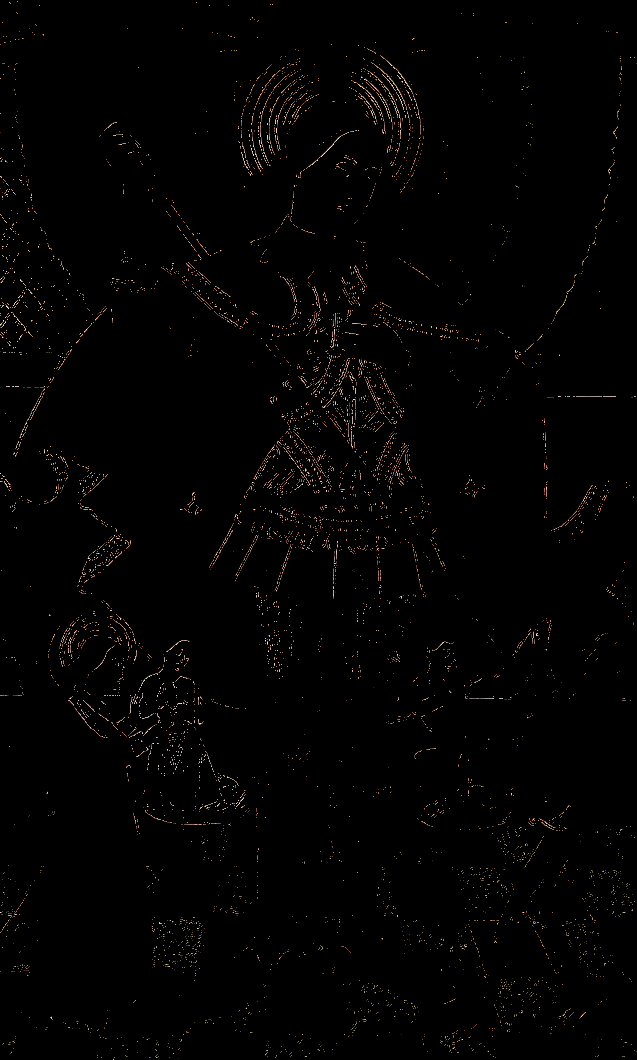
\includegraphics[angle=0,width=0.45\textwidth]{afsnit/afprovning/billeder/thressholds/krafitige_farver/krafite_detalier/1_iteration/700-700.png}
        \label{700-700}}\hspace{1em}
    \subfloat[Original]{
        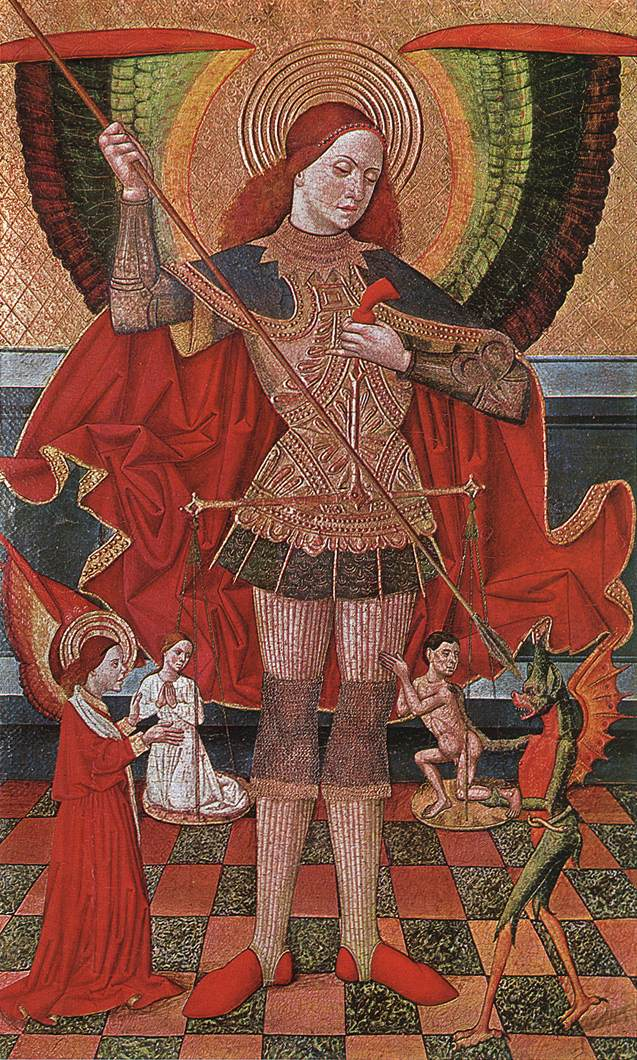
\includegraphics[angle=0,width=0.45\textwidth]{afsnit/afprovning/billeder/thressholds/krafitige_farver/krafite_detalier/kDetalier.jpg}
        \label{kDetalier}}
    \caption[]{Edgedetection på maleriet \ref{kDetalier} som har mange detaliger og kraftige farver, med tærskelværdierne fra 100-100 til 700-700}
     \label{allesammen2}
\end{figure}

\begin{figure}[!h]
    \centering
    \subfloat[300,700]{
        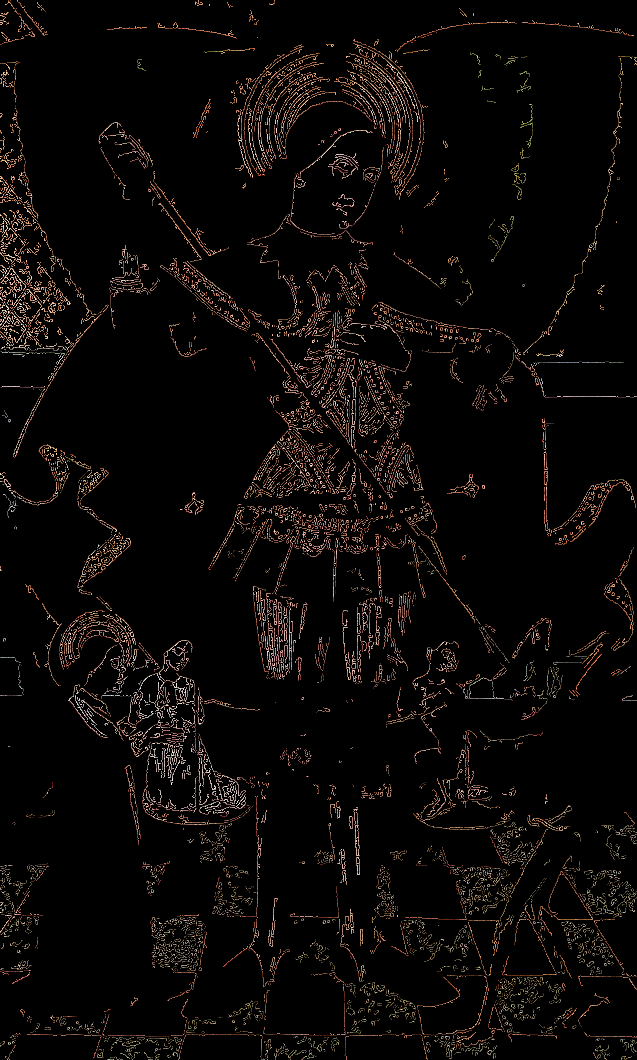
\includegraphics[angle=0,width=0.45\textwidth]{afsnit/afprovning/billeder/thressholds/krafitige_farver/krafite_detalier/2_iteration/300-700.png}
        \label{300-700}}\hspace{1em}
    \subfloat[300,750]{
        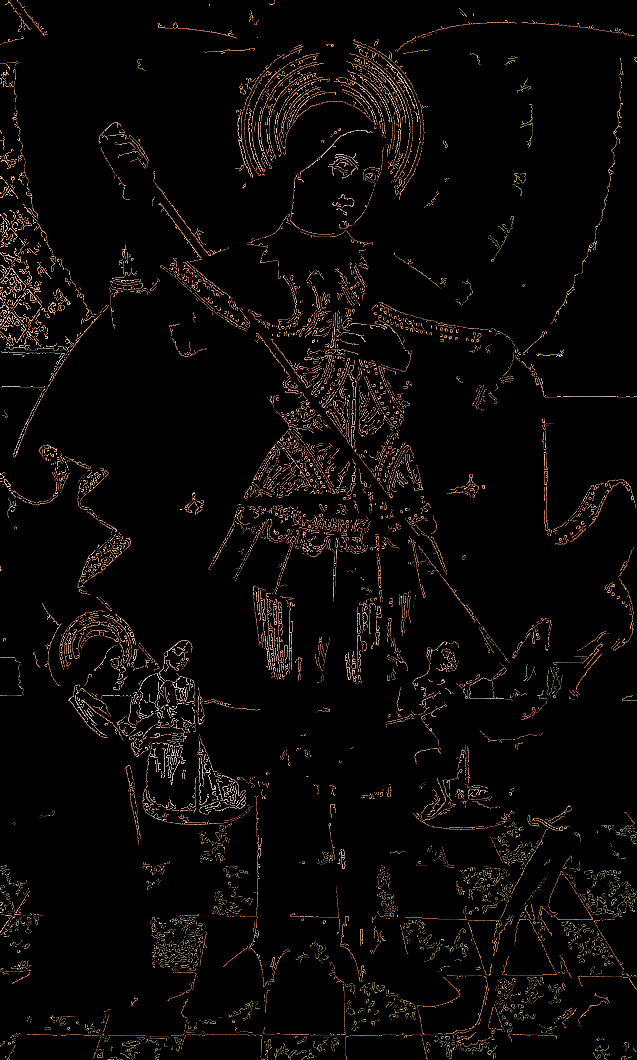
\includegraphics[angle=0,width=0.45\textwidth]{afsnit/afprovning/billeder/thressholds/krafitige_farver/krafite_detalier/2_iteration/300-750.png}
        \label{300-750}}\\
    \subfloat[300,800]{
        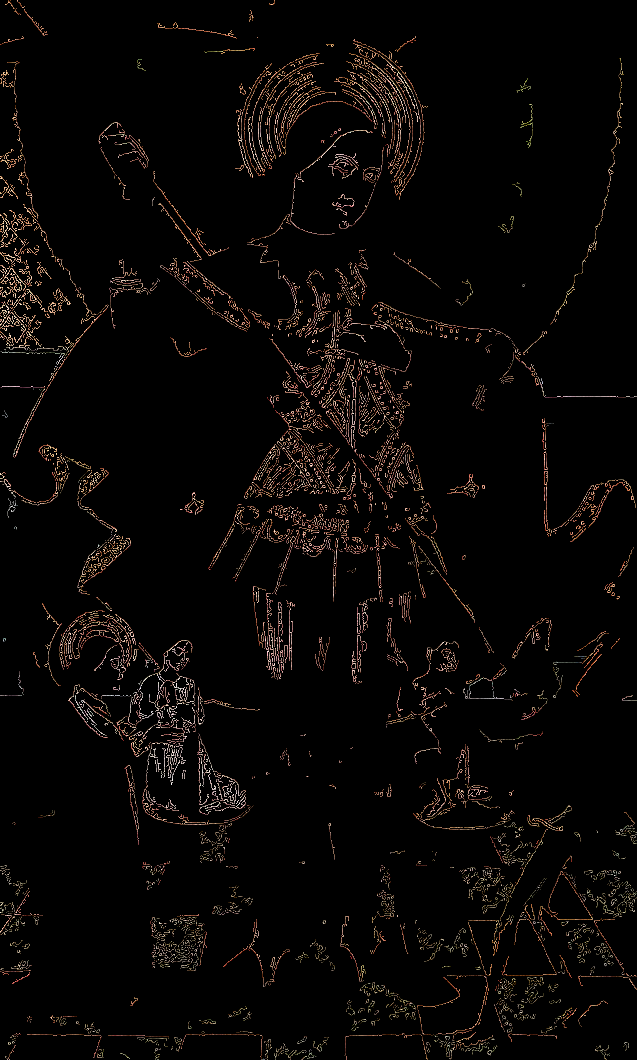
\includegraphics[angle=0,width=0.45\textwidth]{afsnit/afprovning/billeder/thressholds/krafitige_farver/krafite_detalier/2_iteration/300-800.png}
        \label{300-800}}\hspace{1em}
    \subfloat[300,850]{
        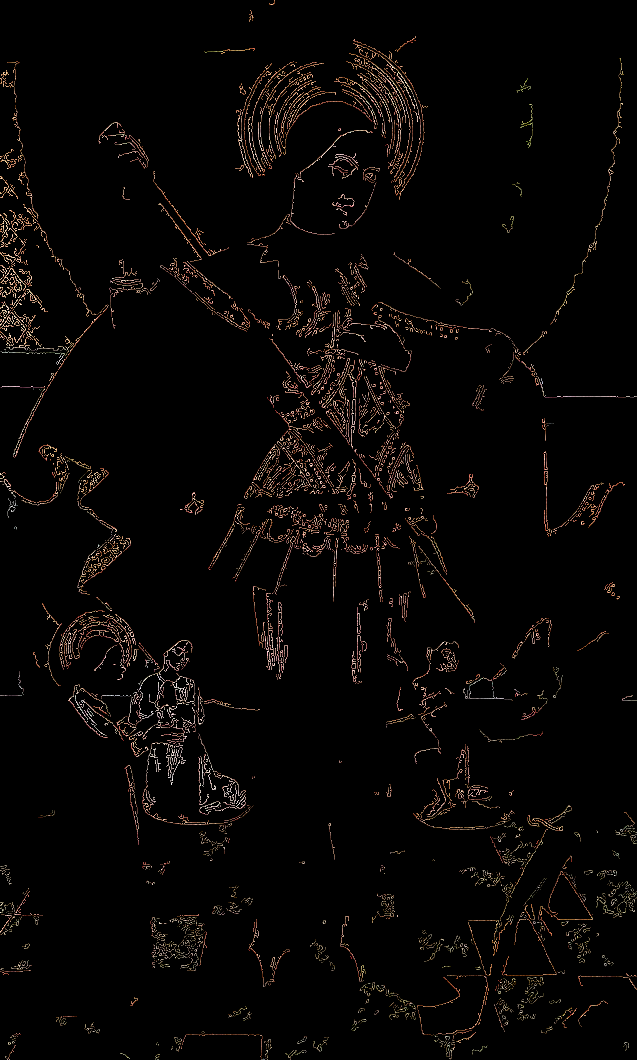
\includegraphics[angle=0,width=0.45\textwidth]{afsnit/afprovning/billeder/thressholds/krafitige_farver/krafite_detalier/2_iteration/300-850.png}
        \label{300-850}}
        \caption[]{Edgedetection hvor de 4 billeder som er intrasante taget med}
     \label{allesammen3}
\end{figure}
 
\begin{figure}[!h]
    \centering
    \subfloat[100,250]{
        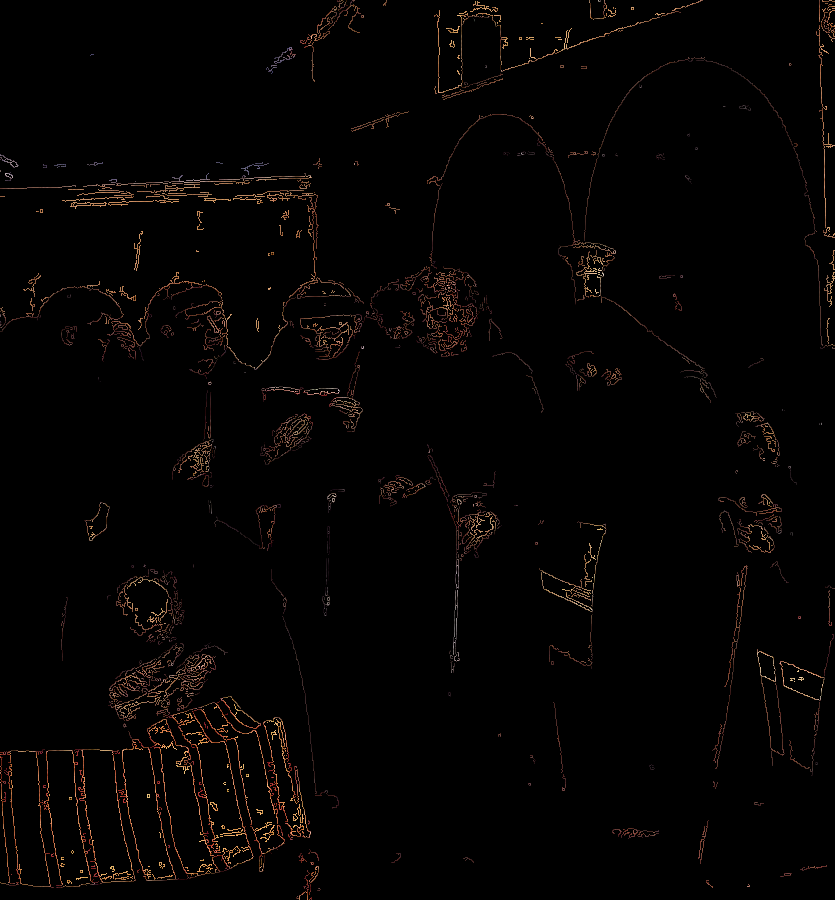
\includegraphics[angle=0,width=0.45\textwidth]{afsnit/afprovning/billeder/thressholds/svage_farver/svage_detalier/2_iteration/100-250.png}
        \label{100-250}}\hspace{1em}
    \subfloat[Orginal]{
        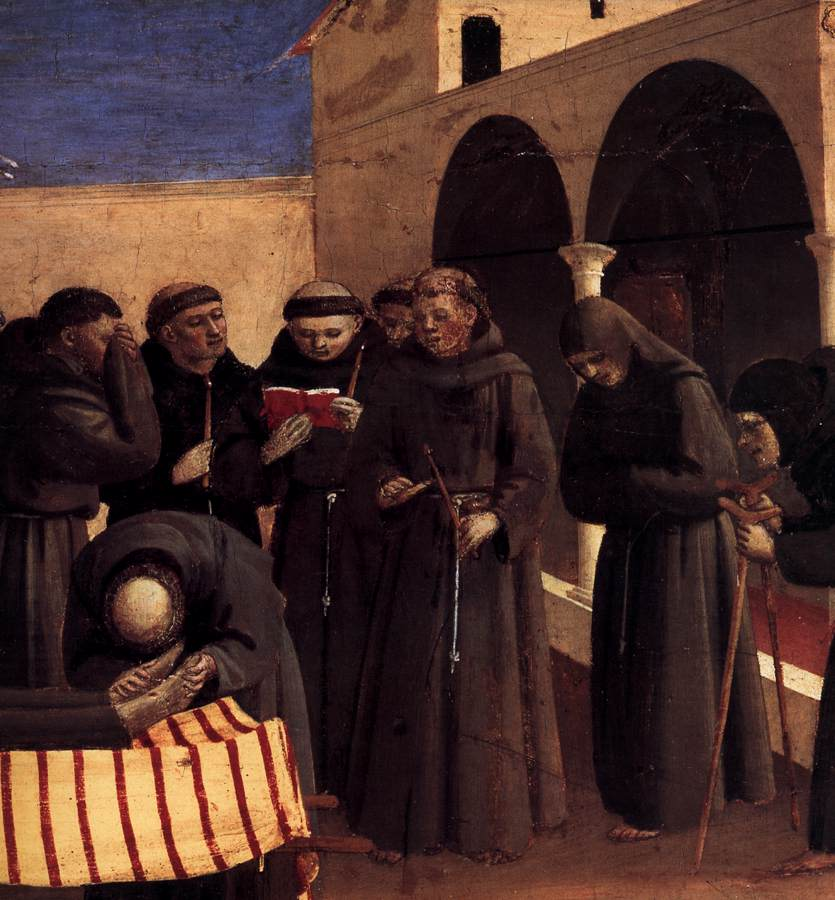
\includegraphics[angle=0,width=0.45\textwidth]{afsnit/afprovning/billeder/thressholds/svage_farver/svage_detalier/sDetalier.jpg}
        \label{Orginal1}}
        \caption[]{Edgedetection på et billedet med svage farver og få detalier, hvor tærskenværdigern [100,250] er den beste}
     \label{en}
\end{figure}

\begin{figure}[!h]
    \centering
    \subfloat[100,240]{
        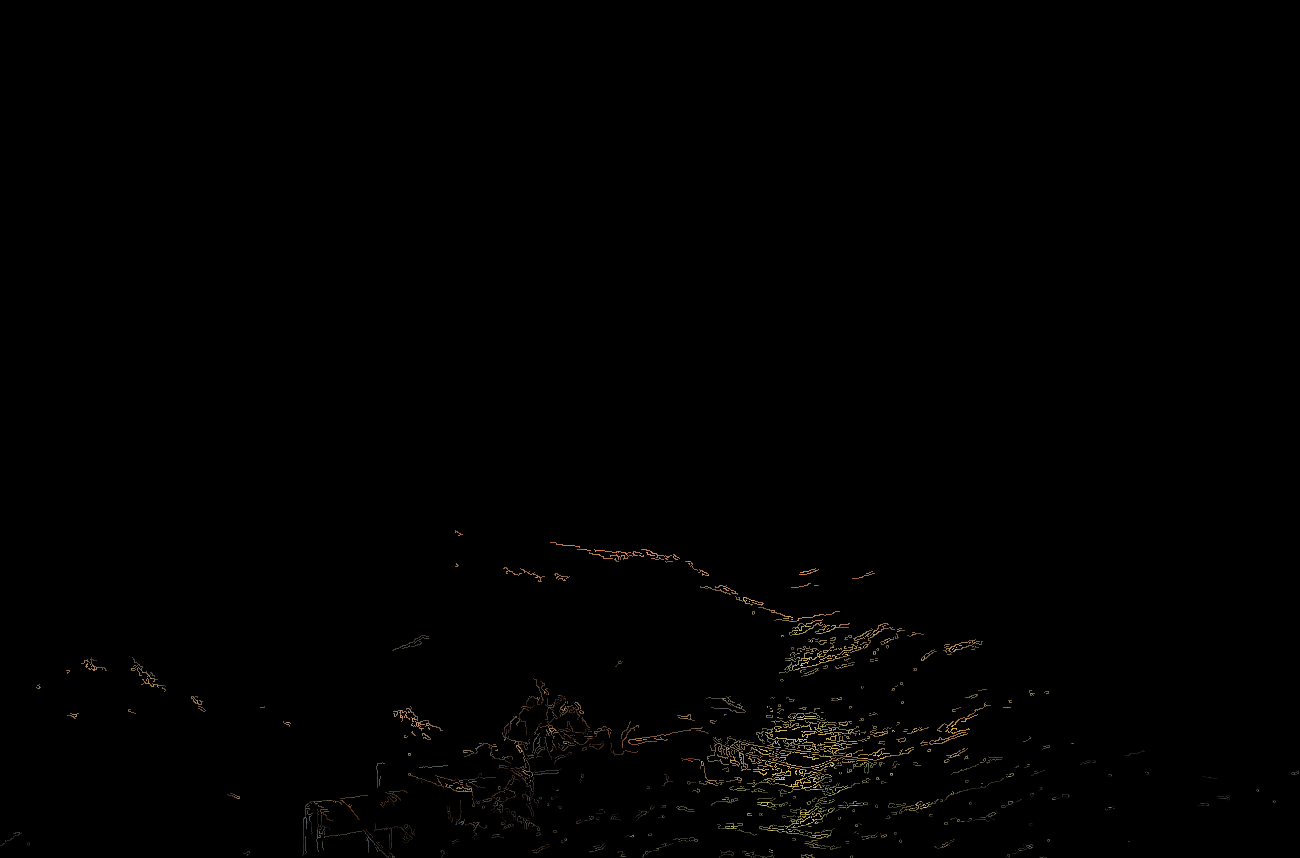
\includegraphics[angle=0,width=0.85\textwidth]{afsnit/afprovning/billeder/thressholds/medium_farver/svage_detalier/2_iteration/100-240.png}
        \label{100-240}}\\
    \subfloat[Orginal]{
        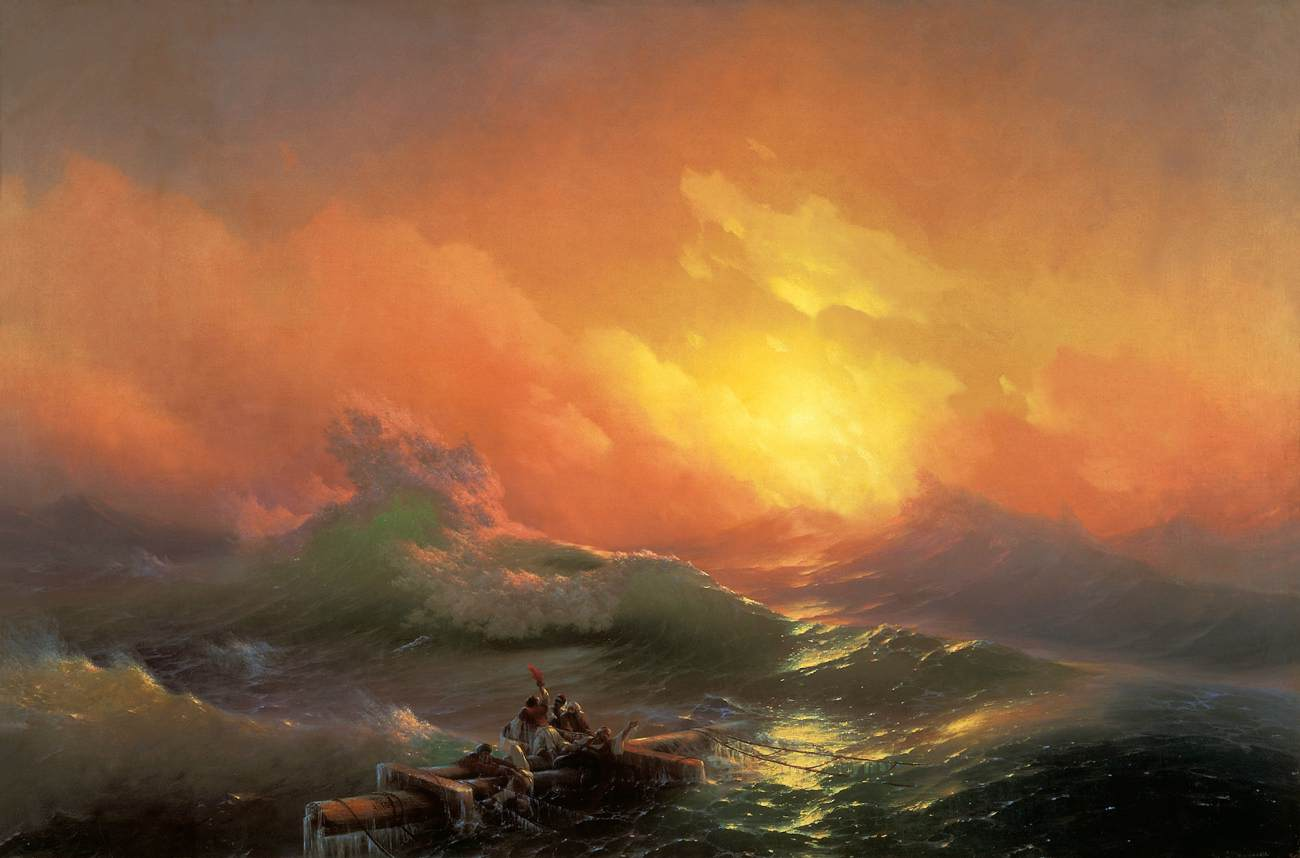
\includegraphics[angle=0,width=0.85\textwidth]{afsnit/afprovning/billeder/thressholds/medium_farver/svage_detalier/sDetalier1.jpg}
        \label{Orginal2}}
        \caption[]{Edgedetection på et billedet med medium farver og få detalier, hvor tærskenværdigern [100,240] er den beste}
     \label{to}
\end{figure}

\begin{figure}[!h]
    \centering
    \subfloat[200,460]{
        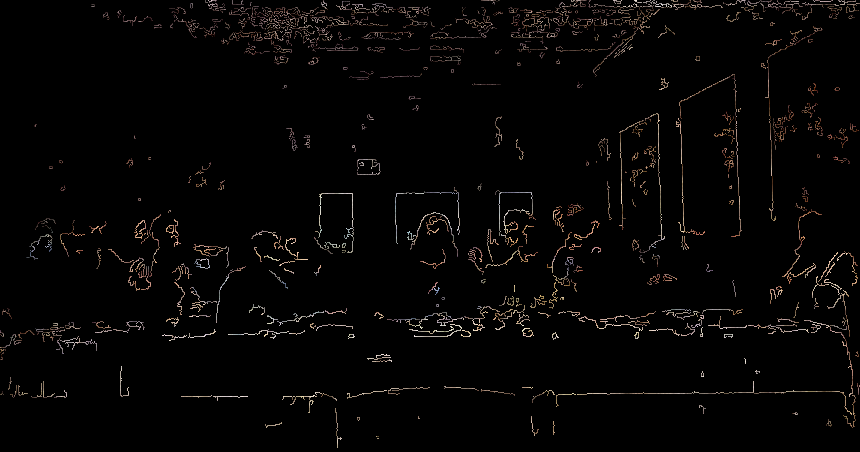
\includegraphics[angle=0,width=0.85\textwidth]{afsnit/afprovning/billeder/thressholds/medium_farver/medium_detalier/2_iteration/200-460.png}
        \label{200-460}}\\
    \subfloat[Orginal]{
        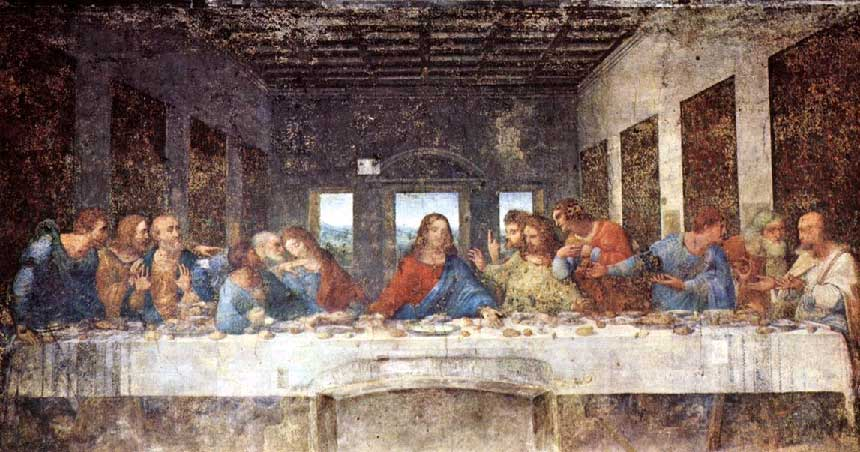
\includegraphics[angle=0,width=0.85\textwidth]{afsnit/afprovning/billeder/thressholds/medium_farver/medium_detalier/mDetalier1.jpg}
        \label{Orginal3}}
        \caption[]{Edgedetection på et billedet med medium farver og medium detalier, hvor tærskenværdigern [200,460] er den beste}
     \label{tre}
\end{figure}

\begin{table}[!h]
    \centering
    \begin{tabular}{| l | l | l | l |} \hline
        & Svage farver 	& Medium farver & Kraftige farver \\ \hline
        Få detalier 		& [100,250]		& [100,240]		& [200,320]\\ \hline
        Medium detalier 	& [100,280]		& [200,460]		& [200,380]\\ \hline
        Mange detalier		& [200,400]		& [200,380]		& [300,750]\\ \hline
    \end{tabular}
    \caption{Beksriv!}
    \label{thressholdsTabelKant}
\end{table}

Som man kan se at tabel \ref{thressholdsTabelKant} gå tærskelværdierne
fra [100,240] til [300,750], så vi kan ikke umiddelbart sætte en fast
tærskelværdi for alle malerier og få at lave en rigtige undersøgelse af
tærskelværdi på malerierne, bliver man nød til at se på mangle flere
malerierne og bestemme deres tærskelværdi og udregne median af de
værdiger, men det vil krave en støre undersøgelse som vi ikke har valt
at gøre, af 3 grunde. 1, det vil kun være en median tærskelværdi få lige
det sæt malerier som vi arbejder på. 2 det vil krave at vi gennemgik
XX(hvor mange) billeder. 3, selv med en median tærskelværdi vil der
stadig være en stor rigge malerier hvor median tærskelværdien ikke vil
være særlige god for. En anden fremgang måde er at regne
tærskelværdierne løbene ud for vært billedet via et program. Men det
problem falder uden for denne opgave og vi vil derfor ikke komme ind på
det. Selv om vi måske ikke kan få det vi helst vil have er der stadig en
del observationer som kan laves ud fra tabellen
\ref{thressholdsTabelKant}. Tærskelværdierne bliver højre nu flere
detaljer og nu kraftigere farverne er. Det virker også som om mange
detaljer vægter lige højt i forholdt til tærskelværdierne en kraftige
farver. Den anden tærskelværdi er ca 2.5 gangen støre en den første
tærskelværdi.

De tærskelværdier som vi har fundet svare til de optimale
tærskelværdier for maleriet, men vi kan godt bruge en værdig som ligger
laver, da metoden floodfill som gør brug af kandtdetektionen resultatset,
god kan tage højde for små kanter, men fejler hvis der ikke er nogle.
Derfor har vi valt at bruger den nederste tærskelværdi som vi har fundet
[100,240] og sænke den lidt til $[78,78 \cdot 2.5 ]$.

\subsection{Afvigelsen af farver i floodfill}
Floodfill har 2 tærskelværdier $lo$ og $up$, som betegner hvor mange pixel
værdier en nabo pixel farver må variere ned og op, en fyldestgørelses
beskrivelse af floodfill findes i afsnit \ref{floodfill}. Vi har tænkt os at
finde en fældes tærskelværdi til brug i vores program. Måde vi gør det på at
ved at observere hvordan floodfill virker med forskellige tærskelværdier og
finde de tærskelværdier som passer bæst til maleriet. Resultatet for
observationen kan ses i tabel \ref{thressholdsTabelFF}, hvor de 9 sammen
kategorier er vist. Et af de malerierne hvor den optimale tærskelværdi er
fundet se i figur \ref{Floodfillbilledet}, så man kan se hvad vi har vurderet
til at være den beste værdi.

\begin{figure}[!h]
    \centering
    \subfloat[8,8]{
        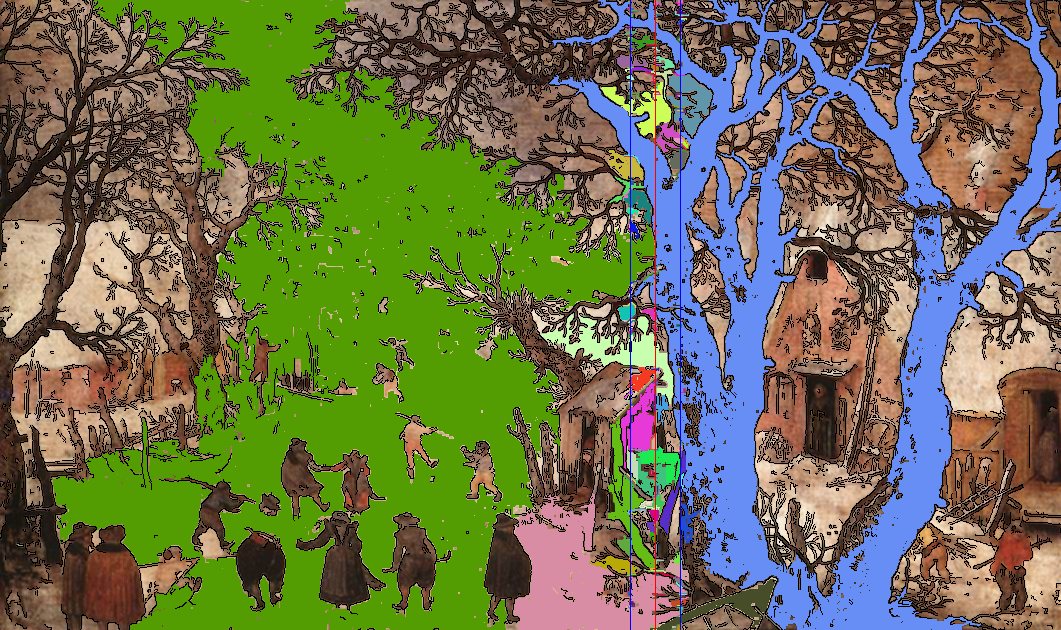
\includegraphics[angle=0,width=0.9\textwidth]{afsnit/afprovning/billeder/thressholds/svage_farver/kraftige_detalier/floodfill/8-8.png}
        \label{8-8}}\\
    \subfloat[Orginal]{
        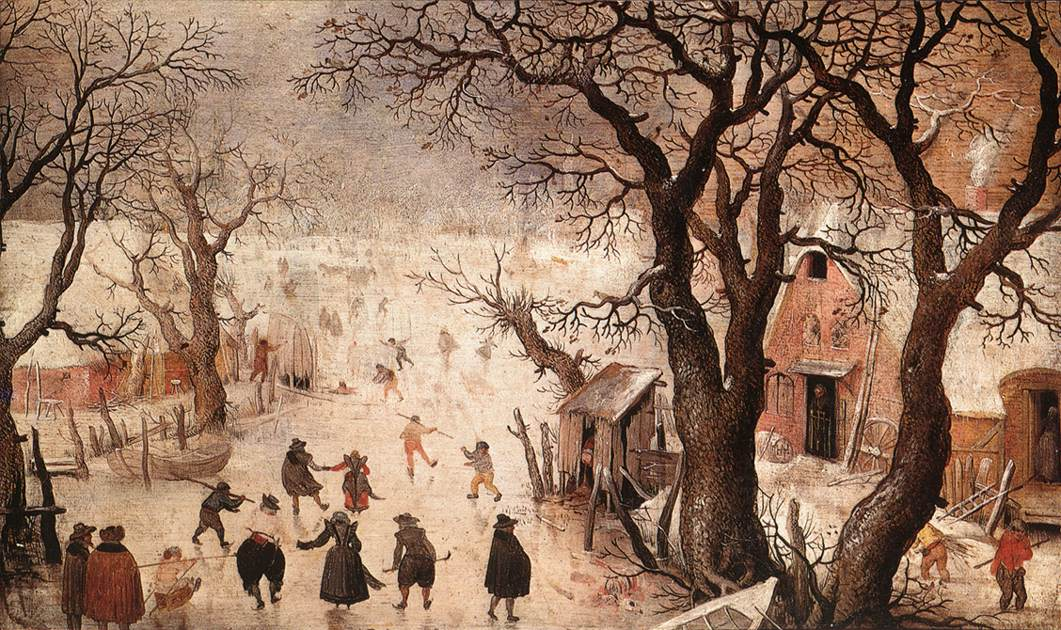
\includegraphics[angle=0,width=0.9\textwidth]{afsnit/afprovning/billeder/thressholds/svage_farver/kraftige_detalier/kDetalier.jpg}
        \label{Orginal4}}
    \caption[]{tærskelværdierne på et billedet med svage farver og kraftige detaljer hvor tærskelværdien [8,8] passer best}
    \label{Floodfillbilledet}
\end{figure}

\begin{table}[!h]
    \centering
    \begin{tabular}{| l | l | l | l |} \hline
        & Svage farver 		& Medium farver & kraftige farver \\ \hline
        Få detalier 		& \textbf{[2,2]}	& [3,3]			& [4,4]\\ \hline
        Medium detalier 	& \textbf{[2,2]}	& \textbf{[5,5]}& \textbf{[2,2]}\\ \hline
        Mange detalier		& [8,8]				& [4,4]			& [7,7]\\ \hline
    \end{tabular}
    \caption{Beskriv!}
    \label{thressholdsTabelFF}
\end{table}

Som man kan af tabellen er nogle af vadierne med fed, begrundelsen for det er
at de vadier er de beste vi kunne finde for billedet, men at de vadier stadig
ikke giver noget som er særlige brugbart, se sektion \ref{floodfilltest}.
værdigerne i tabel fluktuere også en del, så vi har igen samme problem stilling
som i tærskelværdierne ved kantdetektion og har valt at bruge tærskelværdien
[4,4] da dette kommer tættest på gennemsnit.

\section{Regions detektor}
I dette afsnit vil vi afprøve den generelde region detektor, det vil
sige hvad der egentlig bliver fundet inden, vores to metoder sortere
regionerne fra. selve metodes fremgangsmåde er beskravet i sektion
\ref{Sammensetning_af_metoder}, hvor det sideste skrid nå billedet
bliver floodfilldet, derfor vil vi forklare afprøvningen af metode ud
fra billeder som er kommer til dette skridt, hvor tærskelværdierne er
sat til de fundene tærskelværdier. Den første del vil omhandle test på
opbygget billeder og den anden del vil omhandle test på udvalgte
billeder fra vores billedet database.

\subsection{Afprøvning på test billeder}
I dette sektion tester vi på billeder som er konstrueret, men en hvid
baggrund og sorte regioner, det snit vi tester på er indtegnet samt
marginen. I billedet \ref{GRD_test1} er der 5 regioner, hvor 3 af dem bliver
fundet da de ligger i snittet, de 2 regioner som ikke er fundet er
stadig sorte, som man kan se bliver både den er krydser snittet og den
der tangere snittet taget med. I billedet \ref{GRD_test2} er der 3 regioner som
alle bliver fundet, baggrunden, den lille region som ligger inde for
margin, og den store region som kun har en lille del af dens masse inde
i snittet. I billedet \ref{GRD_test3} er der en hoisont som ligger oven på
snittet, begge sider af hoisont linien bliver tegnet med.


\begin{figure}[!h]
    \centering
		\subfloat[4 figure og en bagrun, hvor 2 af figurene og bagrunden er fundet]{
        	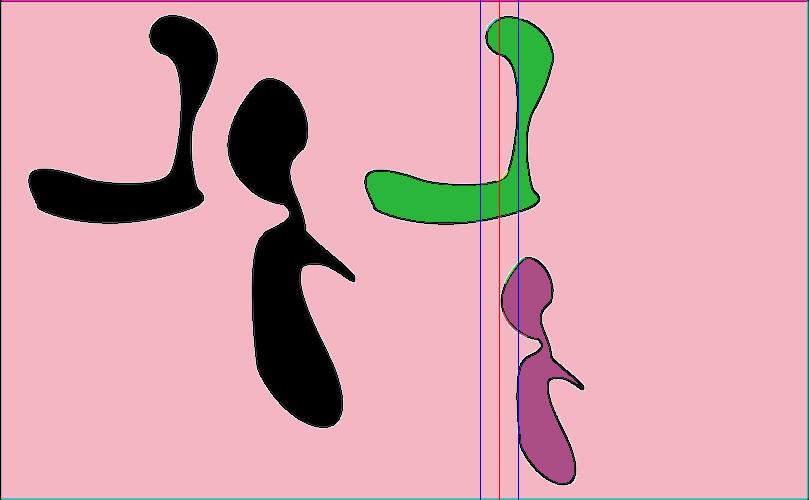
\includegraphics[angle=0,width=0.7\textwidth]{afsnit/afprovning/billeder/region_selector/blob_region_section.png}
        	\label{GRD_test1}}\hspace{1em}
    		\subfloat[En stor figur og en lille figur begge fundet]{
	        	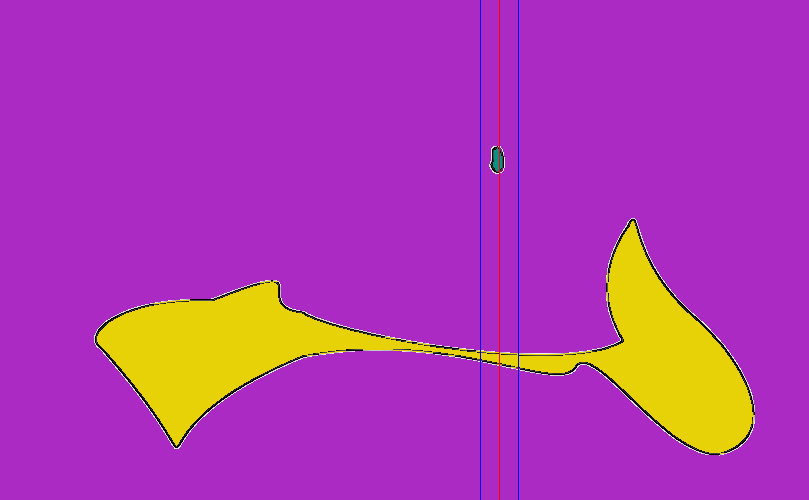
\includegraphics[angle=0,width=0.7\textwidth]{afsnit/afprovning/billeder/region_selector/blob2_region_section.png}
	       	\label{GRD_test2}}\hspace{1em}
    		\subfloat[En hoisont, hvor begge sider er fundet]{
	        	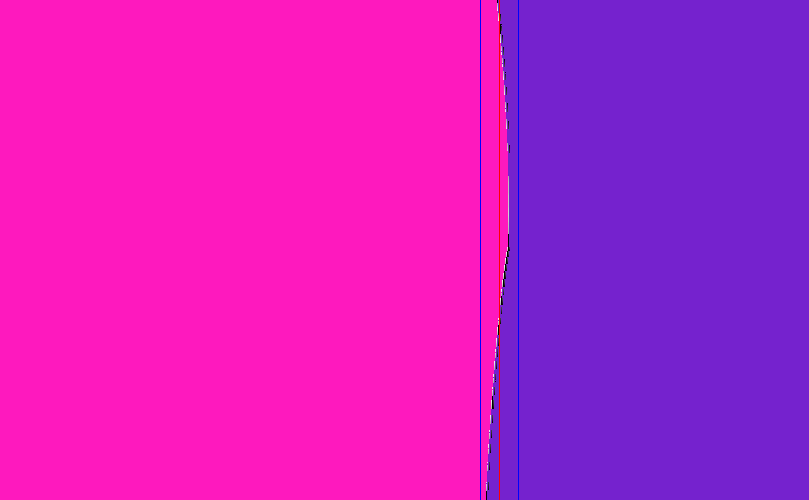
\includegraphics[angle=90,width=0.5\textwidth]{afsnit/afprovning/billeder/region_selector/hoisont_region_section.png}
		       	\label{GRD_test3}}\hspace{1em}
        \caption[]{3 test billeder med bløde former, hvor regien detektor er kørt på dem}
     \label{region_detektor_test}
\end{figure}

I figur \ref{region_detektor_test} er de 3 test billeder afbilledet, de
opføre sig efter de standarter som vi frem satte i afsnit
\ref{}XX(hvilken reference?) 

\subsection{Afprøvning på malerier}
Vi vil afprøve region detektor på 6 udvalte billeder, som vær viser
styrker og svagheder ved region detektoren

\begin{figure}[!h]
    \centering
		\subfloat[Maleri med Kraftige farver og få detaljer]{
        	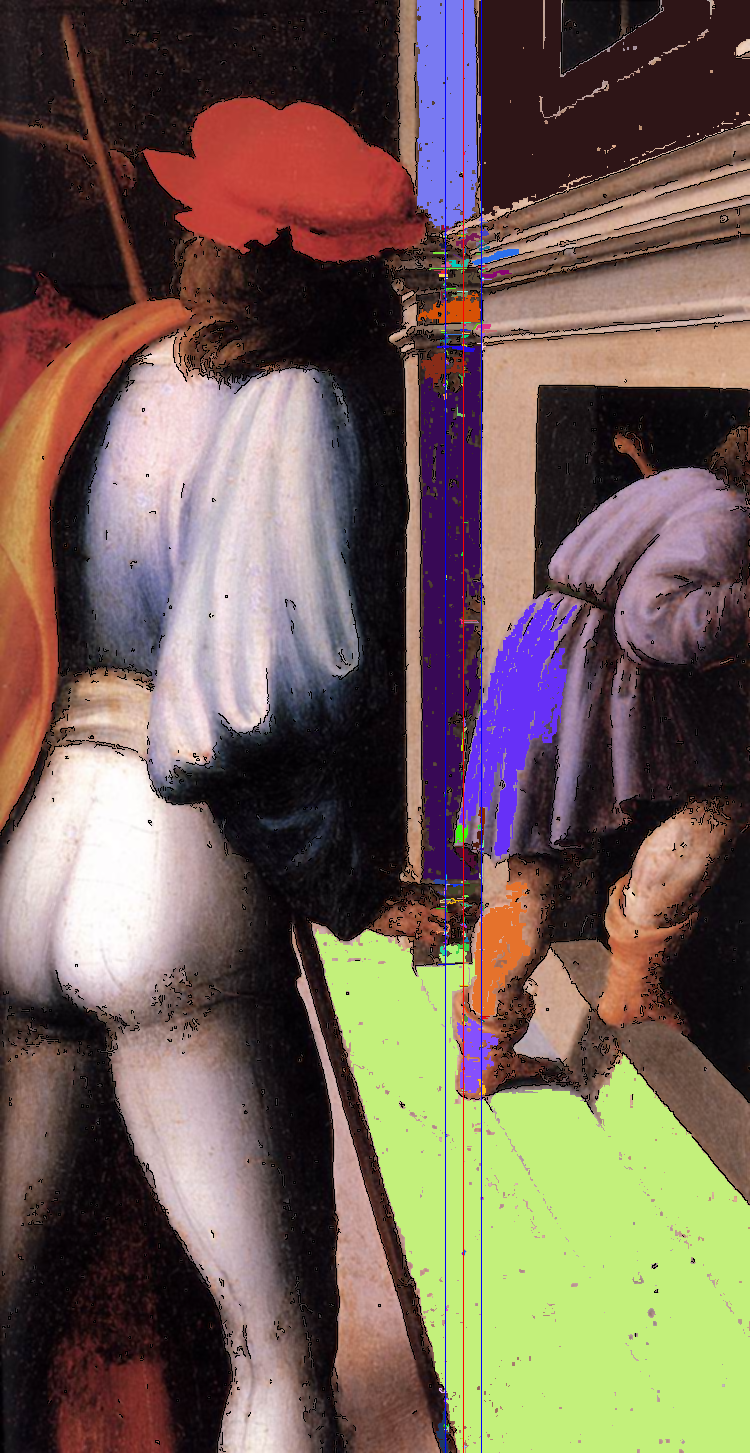
\includegraphics[angle=270,width=1.0\textwidth]{afsnit/afprovning/billeder/thressholds/krafitige_farver/svage_detalier/floodfill/4-4.png}
        	\label{GRD_virker1}}\hspace{1em}
		\subfloat[Medium farver og medium detaljer]{
        	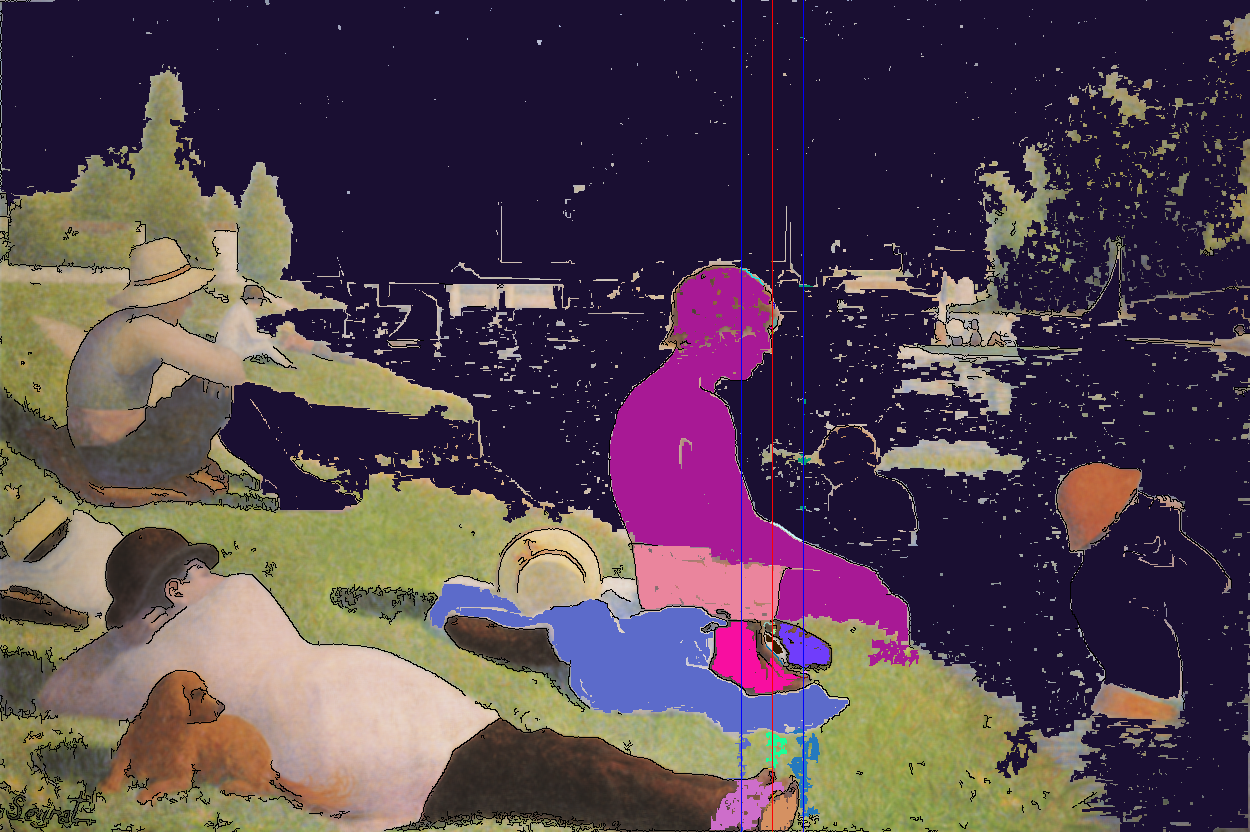
\includegraphics[angle=0,width=1.0\textwidth]{afsnit/afprovning/billeder/4-4.png}
        	\label{GRD_virker2}}\hspace{1em}
        \caption[]{2 malerier hvor regions detektoren virker efter vores ønsker}
     \label{generelde_region_detektor_virker}
\end{figure}

I figuren \ref{generelde_region_detektor_virker} er der 2 malerier, hvor
vores region detektor virker rigtige godt, det første maleri
\ref{GRD_virker1} finder region detektoren 7 store regioner og en masse
små, metoden finder forskel på de forskellige paneler i kaminen og vært
tøj stykke på personen i maleriet er blevet vær deres region, de små
regioner er samlet ved et skift fra et panel til et andet og forstyrrer
ikke de store region ved at gå i gennem dem, man kunne måske have ønsket
at den fylde lidt mere af han karpe ud, men eller et meget godt eksempel
på hvordan den generelde region detektor finde lige det vi vil have den
til at finde. I maleriet \ref{GRD_virker2} finder vi mange af de samme
godt ting, drengen i miden af maleriet er helt udfyldt, en sko og et
håndklæde er også fundet, det er dog vigtigt at ligge mærke til at de
andre personer i vandet, fylder i et med baggrunden, som normalt vil
være en dårlig ting, men som ikke gør noget her da, metoden kun ser
efter regioner i snittet, repræsenteret af den røde linie.
 
\begin{figure}[!h]
    \centering
		\subfloat[Kraftige farver og mange detaljer]{
       	 	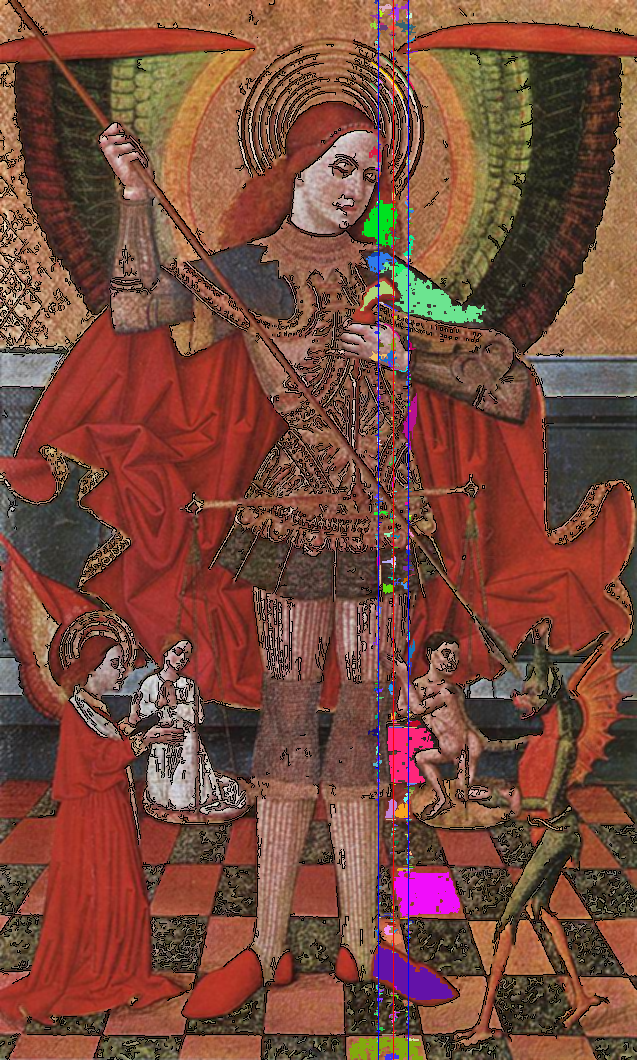
\includegraphics[angle=270,width=0.90\textwidth]{afsnit/afprovning/billeder/thressholds/krafitige_farver/krafite_detalier/floodfill/4-4.png}
		    \label{GRD_virker_nesten1}}\hspace{1em}
    \subfloat[Medium farver og medium detaljer]{
        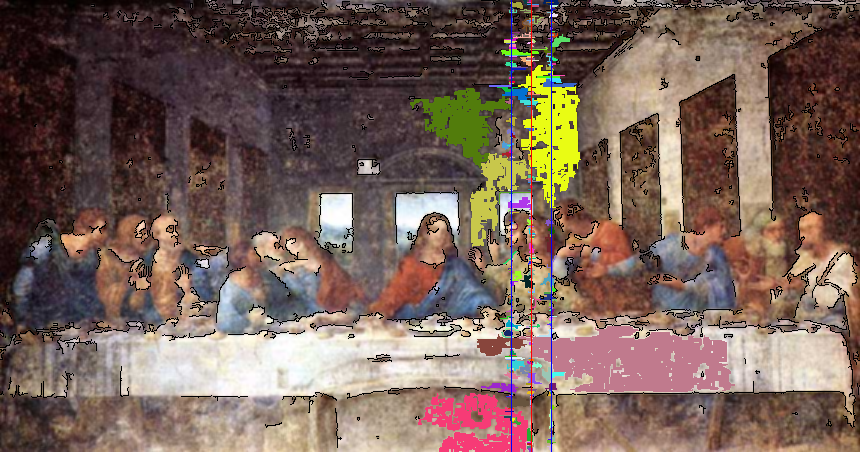
\includegraphics[angle=0,width=0.95\textwidth]{afsnit/afprovning/billeder/thressholds/medium_farver/medium_detalier/floodfill/4-4.png}
        \label{GRD_virker_næsten2}}\\
     \label{generelde_region_detektor_virker_nesten}
     \caption[]{2 malerier hvor regions detektoren ikke helt virker efter vores ønsker men stadig har noget vi kan bruge}
\end{figure}

I figuren \ref{generelde_region_detektor_virker_nesten} er der 2
malerier, hvor vores region detektor ikke virker efter vores ønsker med
stadig har noget vi kan bruge, I maleriet \ref{GRD_virker_nesten1}
bliver der mest fundet små region dog bliver en sko, en skulder og en
flise fundet, hvor vi gerne vil have at personens karpe og arm også blev
fundet, dette skyldes primert at tærskelværdierne for dette billedet er
sat for lavt. Det andet maleri \ref{GRD_virker_nesten2} har nogle af de
samme problematiker, region detektoren finder mest en masse små stykker
af noget som burde hænge sammen. Det vil også kunne løses ved nogle
andre tærskelværdier, men som man også kan se på maleriet er væge og
loftet som egentlige er ret ensfarvet stadig svære for vores region
detektor at fange, det tyder på at en støre sløring godt kunne være
problemløseren få at algoritmen virker på dette maleri. Grunden til at
lige de her 2 bilder er interessante er at ved ændring på tærskelværdier
og sløring kunne vores region detektor virker godt XX(her skal der
billeder hvor det virker), 

\begin{figure}[!h]
    \centering
    \subfloat[Kraftige farver og medium detaljer]{
        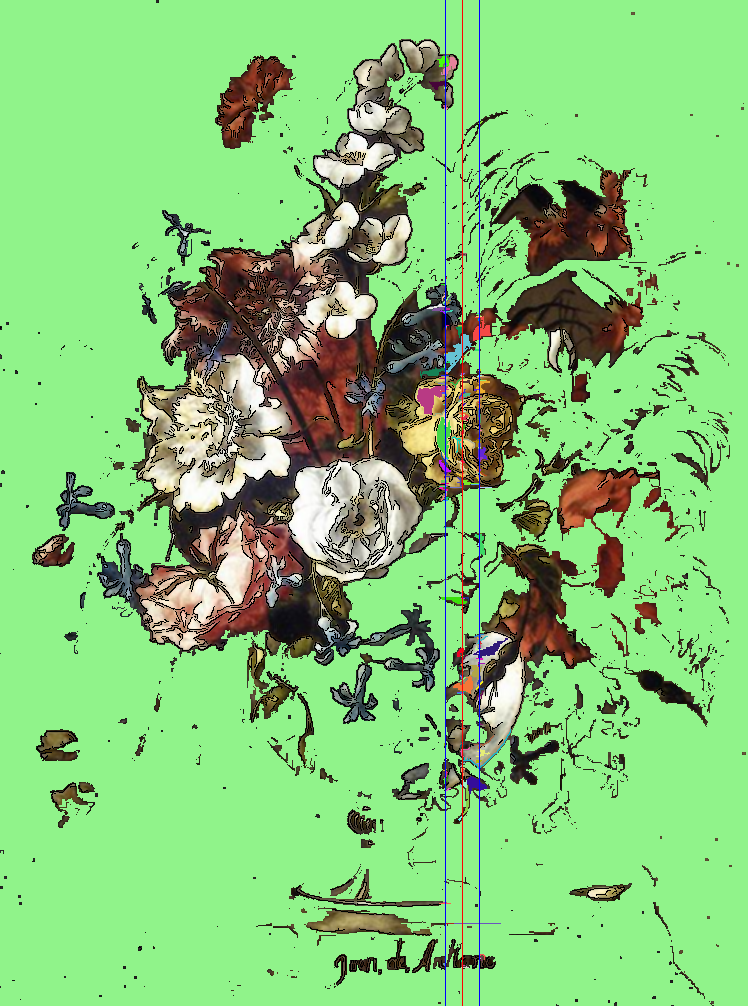
\includegraphics[angle=0,width=0.65\textwidth]{afsnit/afprovning/billeder/thressholds/krafitige_farver/medium_detalier/floodfill/4-4.png}
        \label{GRD_virker_ikke1}}\\
    \subfloat[Svage farver og få detaljer]{
        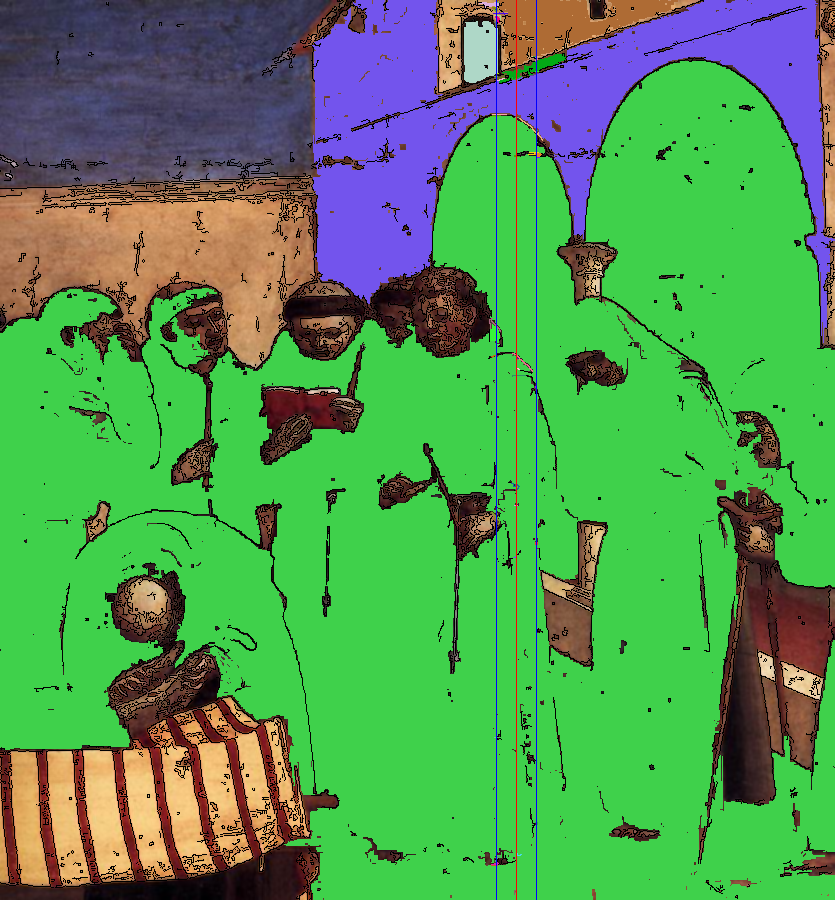
\includegraphics[angle=0,width=0.65\textwidth]{afsnit/afprovning/billeder/thressholds/svage_farver/svage_detalier/floodfill/4-4.png}
        \label{GRD_virker_ikke2}}\hspace{1em}
     \label{generelde_region_detektor_virker_ikke}
\end{figure}

I figur \ref{generelde_region_detektor_virker_ikke} er der 2 malerier
hvor vores region detektor ikke virker særlige godt. I maleri
\ref{GRD_virker_ikke1} er noget af buketten og baggrunden gået i et. På
samme tid er resten af blomsterne i snittet ikke fyldt ud, og selv med
en ændring i tærskelværdierne vil det ikke hjælpe, da en øgning af
tærskelværdierne vil resultere i at flere af blomsterne gå i et med
baggrunden, og en sænkning, vil resultere i at ingen af blomsterne vil
blive detektet. Maleriet \ref{GRD_virker_ikke2} har en anden
problemstiling som vi ikke kan komme uden om, farverne er så mørke og
svage at en ændring i tærskelværdien i floodfill på bare 1 vil få
regiondetektoren til at gå fra at finde ingen regioner til at finde en
stor, som på billedet, dette kan også skyldes at kantdetektionen
tilføje en mørk kan rundt om regionerne, men da maleriet er mørkt i
forvejen hjælper kandetektionen ikke.
XX(jeg kan ikke helt prolamere dette unden at have nogle bileder at bagge det op)


\section{Naive løsning}
%% Bemærk:
%%          Resten af rapporten følger en stil hvor indledninger skrives
%%          med \sffamlily-typen. Denne stil bør også følges her.
%%
{\sffamily
I dette sektion vil vi teste den naive løsning. ved at se om den sortere
de rigtige regioner væk og om løsningen opføre sig på samme måde som vi
har håbet på. Det vil vi gøre ved ført at se på nogle fabrikeret test
billeder, får at se om den naive løsning virker efter meningen og
bagefter vil vi teste på malerierne for at se om den naive løsning kan
bruges i praktisk.
}
  
\subsection{Afprøvning på testbilleder}
Vi vil teste på de samme testbilleder som i sideste afsnit, samt et nyt
testbilleder som blev brugt i forklaringen af den naive metodes, de fire
billeder som vi har valt at test kan se i afsnit \ref{region_detektor}
og billedet \ref{naiv_masse_original} hvor en grån kasse rundt om en
region, betyder at den er valt til at ligge i det gyldne snit af den
naive metode. 

Det første billedet \ref{naiv_blob1}, har fem regioner og hvor tre af
dem blev fundet af reginon detektoren, vores naive løsning har så
sorteret baggrundens regionen og den øverste region i snitte vær, da de
begge krydser marginer og derfor ikke overholder definition
\ref{} . 

\begin{figure}[!h]
	\begin{center}
        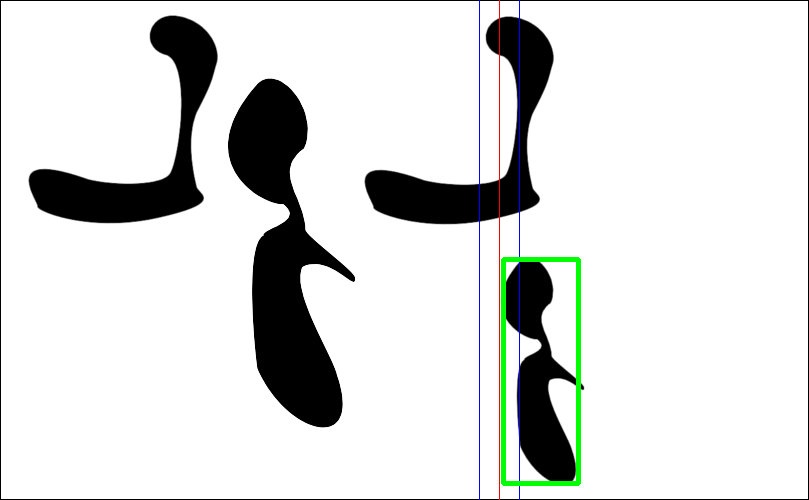
\includegraphics[angle=0,width=0.55\textwidth]{afsnit/afprovning/billeder/naive_losning/naiv_blob1.png}
	\end{center}       
	\caption{Naive algoritme finder en ud af fem regioner}	
	\label{naiv_blob1}
\end{figure}

Det andet billedet \ref{naiv_blob2}, er alle blevet sorteret vær, også
den lille, da den er for lille, derfor ikke overholder definition
\ref{def_interessant} b. 

\begin{figure}[!h]
	\begin{center}
       	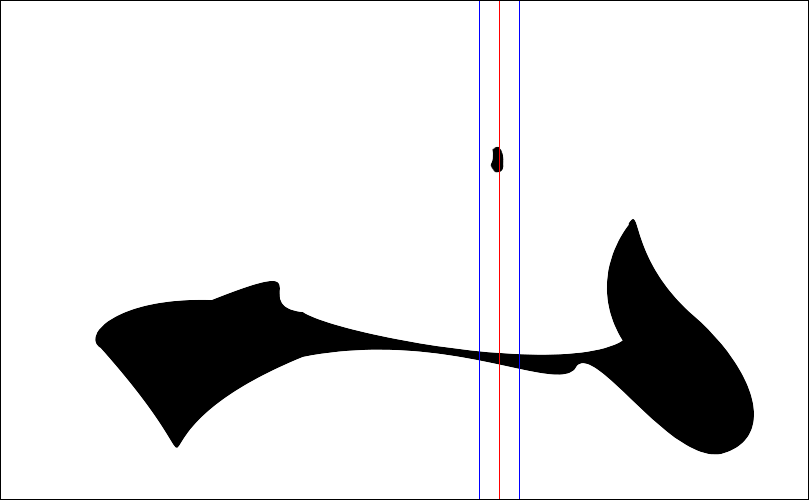
\includegraphics[angle=0,width=0.55\textwidth]{afsnit/afprovning/billeder/naive_losning/naiv_blob2.png}
	\end{center}
	\caption{Værgen den lille region eller den store er fundet} 
   	\label{naiv_blob2}
\end{figure}

I test billedet \ref{naive_hoisont1}, sortere algoritmen
himlen fra, da den krydser margin lidt, men tager jorden med. 

\begin{figure}[!h]
	\begin{center}
       	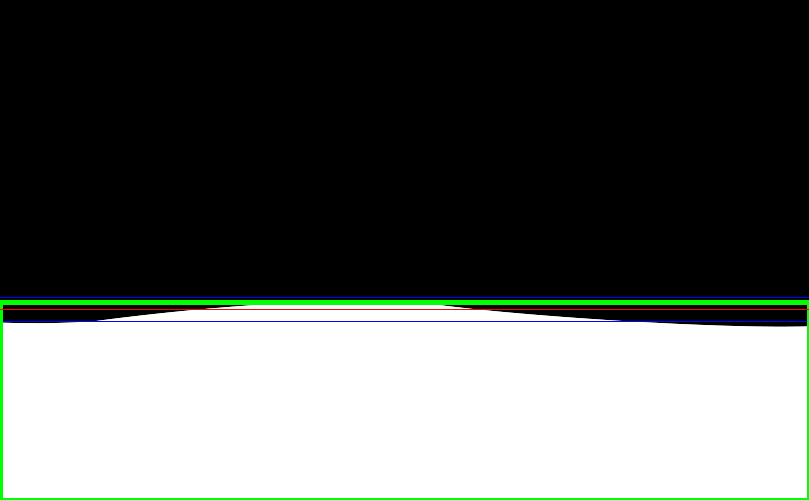
\includegraphics[angle=0,width=0.55\textwidth]{afsnit/afprovning/billeder/naive_losning/naiv_hoisont1.png}
	\end{center}
	\caption{Kun den nederste højrisondt er fundet} 
   	\label{naive_hoisont1}
\end{figure}

\clearpage

\subsection{Afprøvning på malerier}
Vi afprøver den naive algoritme på seks malerier, først på tre malerier,
hvor regions detektoren virker efter vores hensigt og så på ter
malerier, hvor region detektoren ikke virker. Beskrivelsen af hvad der
sker i billedet vil står i caption


\begin{figure}[h!!]
	\begin{center}
		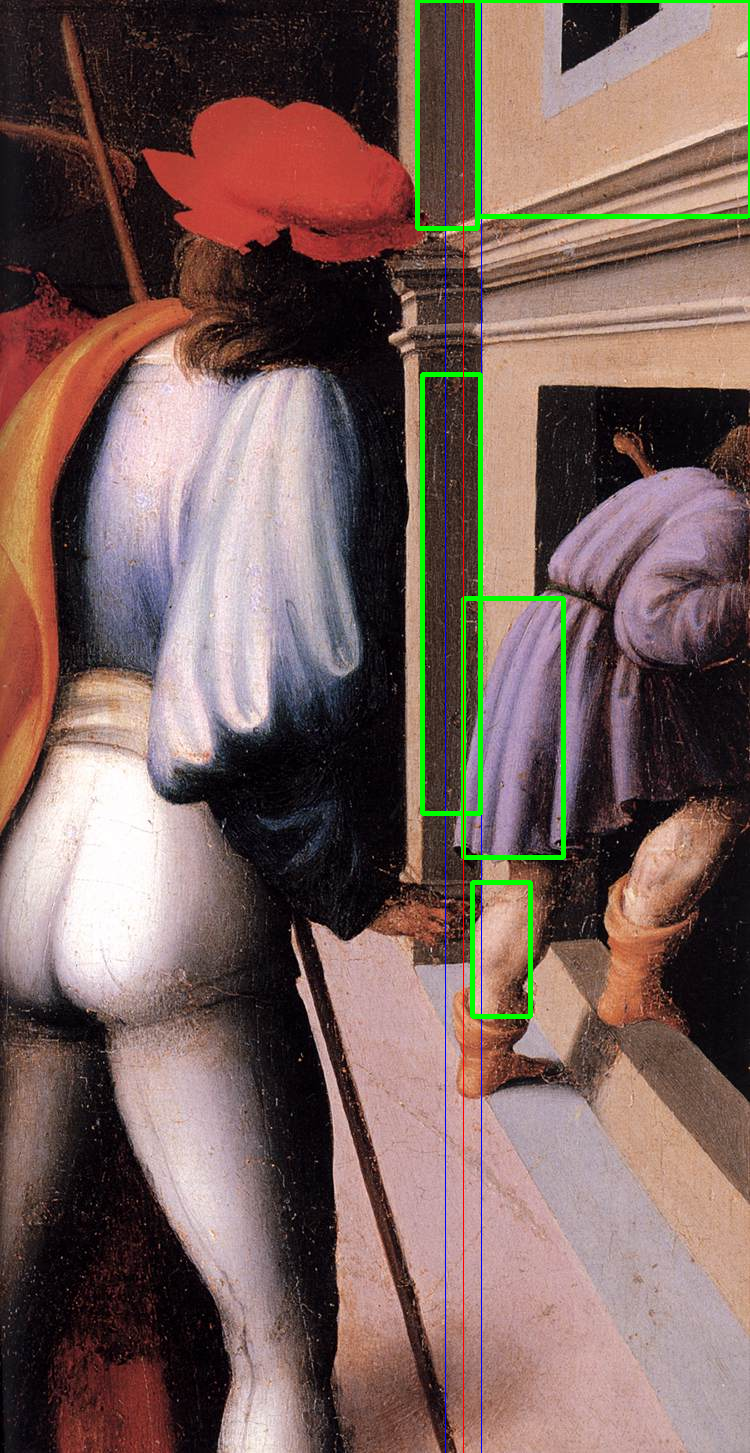
\includegraphics[scale=0.3,angle=0]{afsnit/afprovning/billeder/naive_losning/naiv_kfarver_sdetaljer.png}
	\end{center}
	\caption[]{Fem ud af de seks store regioner fra figur
	\ref{GRD_virker1} valt til at ligge i snittet, skoene er få små til
	at blive taget i betragtning}
	\label{naiv_kfarver_sdetaljer}
\end{figure}

\begin{figure}[h!!]
	\begin{center}
		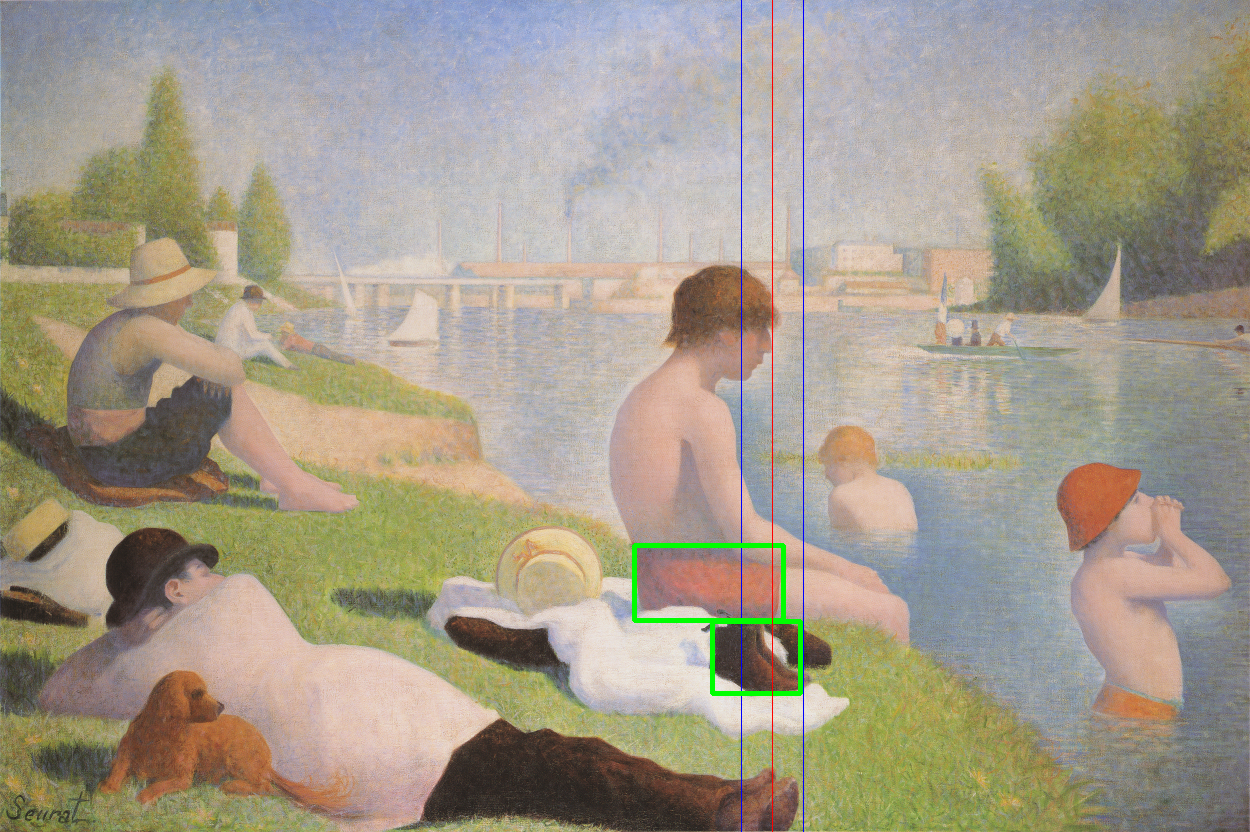
\includegraphics[scale=0.3,angle=0]{afsnit/afprovning/billeder/naive_losning/naiv_mfarver_mdetaljer.png}
	\end{center}
	\caption[]{Bukserne og skoene er tager med af den naive løsning, men
	drengen er sorteret væk da har krydser snittet}
	\label{naiv_mfarver_mdetaljer}
\end{figure}

\begin{figure}[h!!]
	\begin{center}
		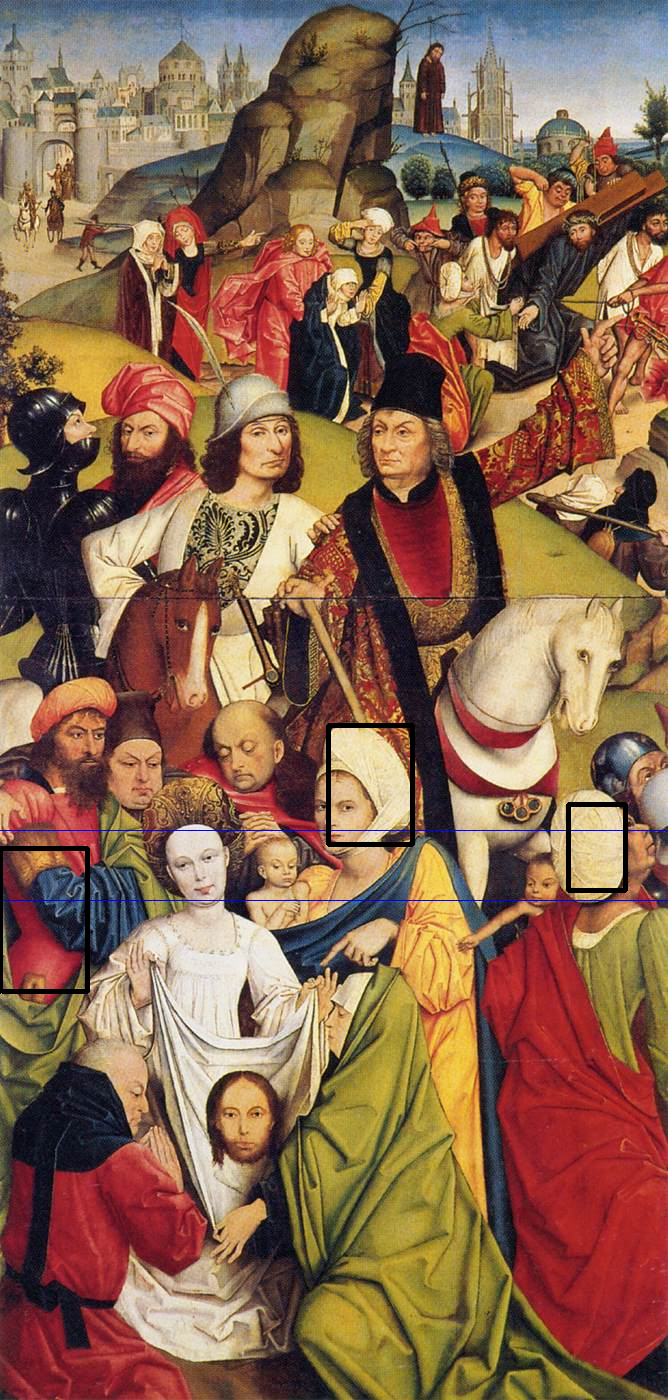
\includegraphics[scale=0.3,angle=0]{afsnit/afprovning/billeder/naive_losning/naiv_kfarver_kdetaljer.png}
	\end{center}
	\caption[]{Et billedet med mange hoder i snittet, hvor to af dem
	bliver godtaget af den naive metode til at ligger i snittet, en
	trøje bliver desværre også taget med. Navn: Christ Carrying the
	Cross. År: 1480. Af: Bosch Hieronymus}
	\label{naiv_kfarver_kdetaljer}
\end{figure}

\begin{figure}[h!!]
	\begin{center}
		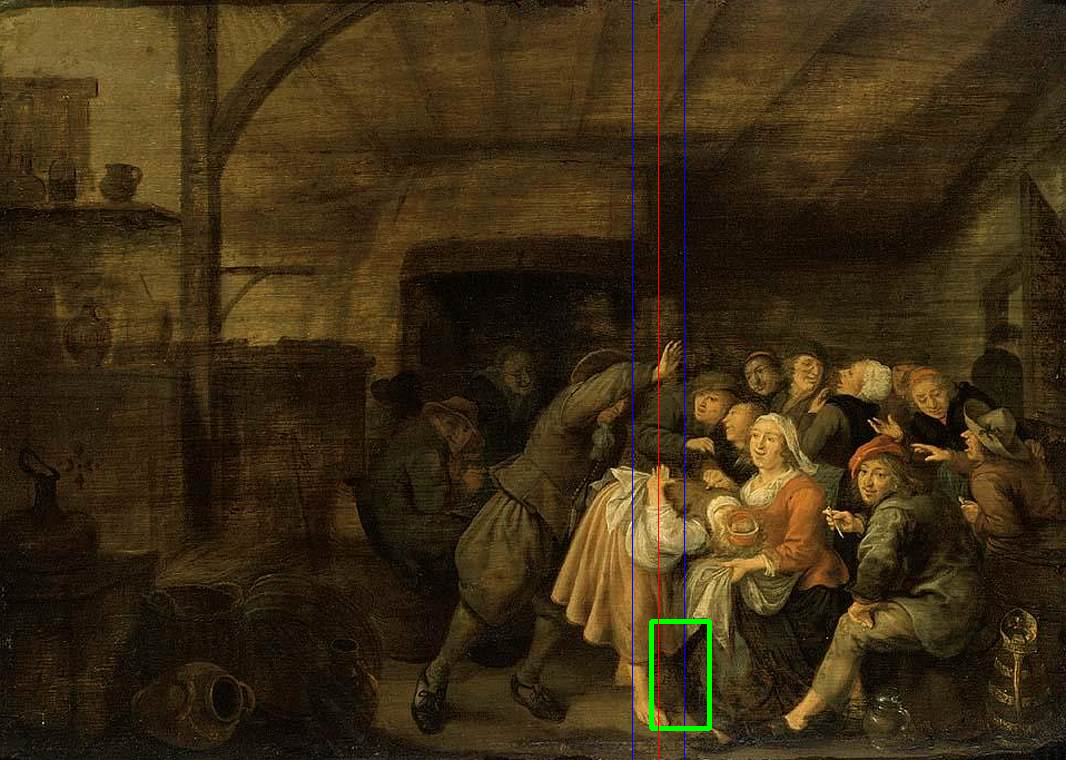
\includegraphics[scale=0.3,angle=0]{afsnit/afprovning/billeder/naive_losning/naiv_virker_ikke1.png}
	\end{center}
	\caption[]{Mallerie hvor region detektor ikke virker, den naive
	løsning godtager tager en region som ligger helt forkert. Navn:
	Peasants in an Inn Playing "La Main Chaude". År: Ukendt. Af:
	Molenaer, Jan Miense.}
	\label{naiv_virker_ikke1}
\end{figure}

\begin{figure}[h!!]
	\begin{center}
		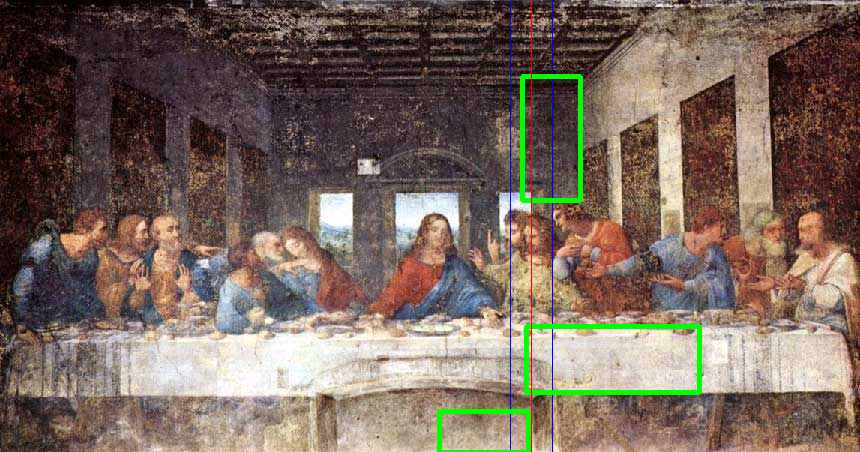
\includegraphics[scale=0.3,angle=0]{afsnit/afprovning/billeder/naive_losning/naiv_virker_ikke2.png}
	\end{center}
	\caption[]{Tre regioner bliver godtaget, selv om de ikke er særlige
	intresante }
	\label{naiv_virker_ikke2}
\end{figure}

\begin{figure}[h!!]
	\begin{center}
		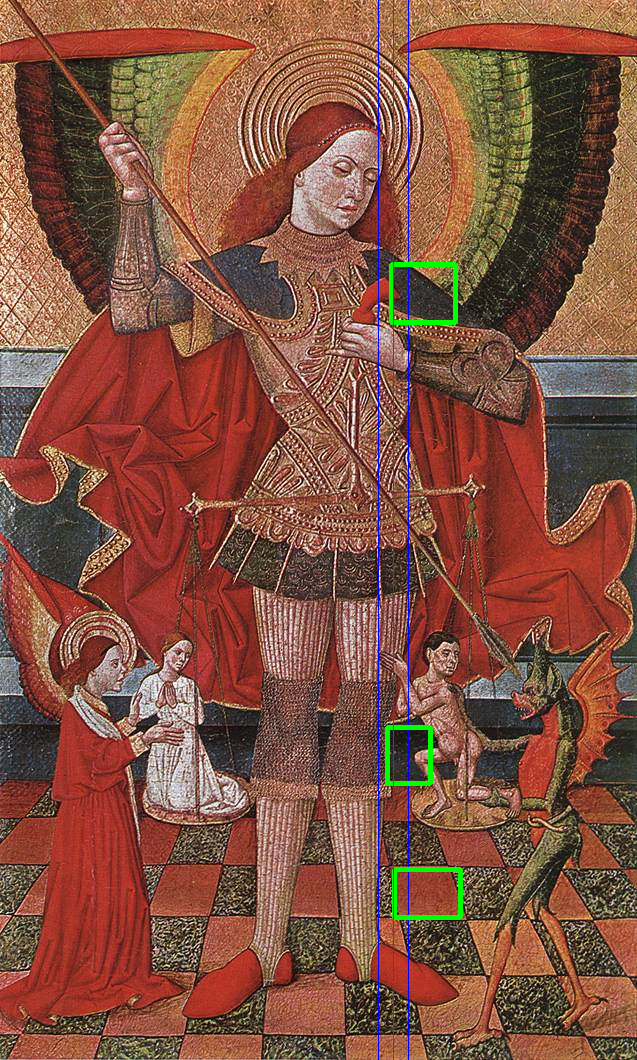
\includegraphics[scale=0.3,angle=0]{afsnit/afprovning/billeder/naive_losning/naiv_virker_ikke3.png}
	\end{center}
	\caption[]{Der bliver fundet tre region, hvor kun en af dem passer
	på en ting i billedet}
	\label{naiv_virker_ikke3}
\end{figure}
\clearpage

\subsection{Konkulution}
Det virker som om den naive løsning virker efter vores entationer dog
med nogle få falske positive, hvis region detektoren virker på
malerierne, dog fejler den på malerier hvor region detektoren fejler, og
kommer med en masse falske positive.

\section{Udvidet løsning}


}

% vim: set tw=72 spell spelllang=da:


\chapter{Implementation\label{chap_implementation}}
%% Bemærk:
%%          Programmeringssprog skrives med stort begyndelsesbogstav (første gang fed, (hvis gennemgående))
%%          Pakker skrives med kursiv (\emph{})
{
{\sffamily Dette kapitel har til formål at gennemgå, hvordan
principperne fra kapitel \ref{chap_indledning} og metoderne fra kapitel
\ref{chap_detektion} er blevet implementeret, samt hvilke problemer, der
kan opstå i denne forbindelse. Vi vil også komme ind på, hvordan
resultater --- som dem vist i kapitel \ref{chap_afproevning} ---
repræsenteres og gemmes, samt på hvordan vi kører analysen på malerierne
i vores database.  Vi forklarer programmet, og metoderne deri, ``fra
bunden og op'', dvs. at vi bevæger os fra lille kompleksitet, hvor der
lægges ud med de helt grundlæggende strukturer og principper, til stor
kompleksitet, når de enkelte dele sættes sammen.  I bilag
\ref{appendix_struktur} er vedlagt en oversigt over programmets opdeling.
Indledningsvis kigger vi på, hvilke programmeringssprog og biblioteker
vi benytter os af.
}

\section{Programmeringssprog og biblioteker\label{section_programmeringssprog}}
{
{\sffamily Ved valg af programmeringssprog har vi først og fremmest lagt
vægt på at kunne udarbejde en prototype hurtigt og bruge et sprog, som
er let at gå til. Det valgte sprog skal også gøre det nemt at udvide den
endelige implementation. Vi har også gerne villet undgå at skulle
konstruere komplicerede datastrukturer for relativt simple metoder, både
af hensyn til tidspresset og til implementationens kompleksitet. Af
ovenstående grunde har vi besluttet at udarbejde vores løsning i
programmeringssproget \textbf{Python}\cite{PythonLanguage}. Vores
erfaring er, at dette sprog er yderst velegnet at skrive forholdsvis
avancerede prototyper i.
}

\subsection{OpenCV}
Til udførelse af billedmanipulationer benytter vi os af et bibliotek
skrevet i C og C++, der hedder \emph{OpenCV}\cite{OpenCV}. Biblioteket
er udviklet af Intel og tilbyder, udover et solidt udvalg af algoritmer,
bindinger til Python\cite{OpenCVPython}. Endelig er det meget
veldokumenteret og giver referencer til publikationer om bibliotekets
algoritmer. Biblioteket er udviklet med specielt henblik på real-tids
behandling af billeder, f.eks. med et videokamera som kilde, men det
egner sig også til brug på enkelte billeder.  \emph{OpenCV} tilbyder
mange brugbare datastrukturer med hensyn til arbejdet med billeder i
Python.

Der er også andre biblioteker til billedbehandling i Python. Her kan
nævnes \emph{PIL} (Python Imaging Library)\cite{PIL} og
\emph{PythonMagick} (ImageMagick bindings)\cite{PMck}, men de er ikke
nær så grundige som \emph{OpenCV}.

\subsubsection{Andre muligheder}
Der er to helt oplagte muligheder, med hensyn til programmeringssprog,
når man taler om billedbehandling, nemlig Matlab\cite{MatlabLang} og
dets Open Source-alternativ Octave\cite{Octave}. Disse sprog blev dog
valgt fra, da vores samlede erfaring med udvikling i disse sprog ikke
var stor nok.  Endvidere finder vi, at disse sprog, på trods af, at de
især egner sig til den type beregninger, vi skal lave, er besværlige at
lave større programmer med. Matlab og Octave er dog blevet brugt til at
sammenligne resultater og teste alternative metoder med.

Da \emph{OpenCV} er skrevet i C/C++, ville det også være oplagt at bruge
et af disse sprog. Vores erfaring er dog, at man let kommer til at bruge
mere tid på at konstruere de fornødne datastrukturer og hjælpemetoder,
end på at fokusere på opgavens kerne. En senere implementation, med
fokus på køretid, kunne med fordel implementeres i C/C++, da man så
ville have fuld kontrol over, hvilke strukturer der bliver brugt i
programmet.

\subsection{Værktøjer til databasen}
Vi bruger \textbf{SQLite}\cite{Sqlite} til selve databasen, hovedsagelig
fordi der ikke kræves nogen videre konfiguration af en sådan database.
Den underliggende database er dog underordnet, da vi bruger
Python-pakken \emph{SQLObject}\cite{Sqlobject}, som giver et
abstraktionslag til en bred vifte af databaser. Vi opretter blot de
tabeller, vi ønsker at have i databasen, som klasser i Python og får
ligeledes en sådan klasse tilbage, når der laves forespørgsler til
databasen. Da \emph{SQLObject} klarer al kommunikation med databasen, er
det derfor muligt at skifte den underliggende database ud, hvis man
ønsker det. SQLite har endvidere den umiddelbare fordel, at selve
databasen eksisterer som en fil i filsystemet.  Det er derfor en let sag
at tage sikkerhedskopier af databasen uden alt for meget besvær.

\subsection{Andre værktøjer}
Vi har gjort brug af statistikprogrammet \textbf{R}\cite{Rlang} til at
behandle og præsentere vores resultater i kapitel \ref{chap_resultater}.
Da programmet primært er blevet brugt som hjælpeværktøj, til at
producere grafer, vil vi ikke komme nærmere ind på, hvordan disse
hjælpeprogrammer er blevet udviklet.

}

% vim: set tw=72 spell spelllang=da:


\section{Billedbehandling med OpenCV\label{section_impBilledbehandling}}
{
{\sffamily I det følgende, kaster vi et detaljeret blik på
billedbehandlingsmetoderne i programmet. Efter en teknisk
introduktion til digitale billeder, vises hvilke datastrukturer og
metoder \emph{OpenCV} stiller til rådighed, og hvordan disse bruges, til
at udtrække regioner i digitale billeder. Endeligt vil vi undersøge,
hvilke svagheder vores implementation, til udtrækning af regioner, har.
}

\subsection{Digitale billeder}
I afsnit \ref{section_kort_intro} blev der givet en kort introduktion
til den digitale repræsentation af billeder. Vi antog, at en pixel kunne
antage værdier i mængden $\{0, 1\}$. I praksis, kan pixels godt tage
andre værdier. Vi arbejder med billeder, hvor værdien for hver pixel, er
repræsenteret ved tre 8 bit størrelser --- hver især med værdier i
mængden $\{0, 1, 2, \cdots, 254, 255\}$. Sammensætningen af de tre
værdier, som beskrives som kanaler eller farvebånd, kaldes for en
RGB-farve, hvor tallene repræsenteret ved $(R,G,B)$ angiver mængden af
hhv. rød, grøn og blå farve i en pixel. Et sådant billede, kaldes for et
RGB-billede. Vores korpus består af sådanne RGB-billeder med 8 bits, og
vi benytter derfor også denne repræsentation internt. Der er enkelte
undtagelser, hvor der kun bruges én kanal, således at vi arbejder med
gråtonebilleder. For en uddybende forklaring om billeders
repræsentation, refereres igen til \cite{SIOlsen}.

\marker{Hvordan repræsenteres billeder i \emph{OpenCV}? Skriv det
her.}{Husk det!}
Noget med matricer og arrays og Python og \emph{OpenCV}.

\subsection{Resultaters struktur\label{resultat_struktur}}
Indledningsvist vil vi introducere nogle vigtige datastrukturer, som vi
bruger fra \emph{OpenCV}. Alle datastrukturer og metoder fra
\emph{OpenCV}, er prefikset med ``cv'', hvilket gør det let, at skelne
vores egne metoder fra dem der er givet i \emph{OpenCV}.  Der
præsenteres i det følgende en notation for datastrukturer.  Notationen
er underlagt strukturen vist i \eqref{types_class}.
\begin{multline}
    \textbf{class~} [\textit{name}] = \{ \\
    \shoveleft{\qquad[\textit{type}] : [\textit{varName}]} \\
    \shoveleft{\}}\shoveright{}
    \label{types_class}
\end{multline}
I \eqref{example_class} ses et eksempel på en struktur kaldet
\textbf{ExampleClass}.
\begin{multline}
    \textbf{class~} \textrm{ExampleClass} = \{ \\
    \shoveleft{\qquad\textbf{int} : \textit{intValue}} \\
    \shoveleft{\qquad\textbf{string} : \textit{stringValue}} \\
    \shoveleft{\qquad\textbf{int[2]} : \textit{arrayValues}} \\
    \shoveleft{\}}\shoveright{}
    \label{example_class}
\end{multline}
Når en type har et suffiks på formen $\textit{type}[i]$, hvor $i$ er et
heltal, betyder det, at dette er en liste af længde $i$ af typen
\textit{type}.  Bemærk, at en strukturs navn bliver skrevet med fed
skrift i brødteksten, når der refereres til en sådan. Ligeledes vil en
strukturs navn blive skrevet med fed i pseudokoden, hvis der refereres
til den. Vi kan definere en ny struktur \textbf{NewClass}, som viser
dette, i \eqref{new_class} herunder.
\begin{multline}
    \textbf{class~} \textrm{NewClass} = \{ \\
    \shoveleft{\qquad\textbf{ExampleClass} : \textit{exampleInstance}} \\
    \shoveleft{\qquad\textbf{string} : \textit{stringValue}} \\
    \shoveleft{\}}\shoveright{}
    \label{new_class}
\end{multline}
Vi vil nu beskrive de vigtigste datastrukturer, som vi bruger, med
ovenstående notation.

\subsubsection{cvScalar}
Strukturen \textbf{cvScalar} fungerer egentlig blot som en almindelig
liste med værdier. En instans af \textbf{cvScalar} kan dog kun indeholde
1, 2, 3 eller 4 værdier. Strukturen vist i \eqref{cvScalar_class} har fire
værdier.
\begin{multline}
    \textbf{class~} \textrm{cvScalar} = \{ \\
    \shoveleft{\qquad\textbf{double[4]} : \textit{value}} \\
    \shoveleft{\}}\shoveright{}
    \label{cvScalar_class}
\end{multline}
I \emph{OpenCV}, og vores implementation i øvrigt, bruges strukturen
blandt andet til RGB-farver og tærskelværdier. Til RGB-værdier bruger
\emph{OpenCV} også strukturen \textbf{CV\_RGB}, men dette er reelt blot
en instans af \textbf{cvScalar}.

\subsubsection{cvPoint}
Strukturen \textbf{cvPoint} har til formål at beskrive punkter i det
to-dimensionelle plan. Den er givet i \eqref{cvPoint_class}.
\begin{multline}
    \textbf{class~} \textrm{cvPoint} = \{ \\
    \shoveleft{\qquad\textbf{int} : \textit{x}} \\
    \shoveleft{\qquad\textbf{int} : \textit{y}} \\
    \shoveleft{\}}\shoveright{}
    \label{cvPoint_class}
\end{multline}
Strukturen er simpel, men er en meget central del af implementationen.
Den bruges blandt andet til at angive snit i billedet samt fortælle
floodfill hvor vi skal male og skifte farve.

\subsubsection{cvRect}
Denne struktur beskriver et rektangel, ved at angive dets øverste venstre
hjørne og dimensioner. Strukturen vises i \eqref{cvRect_class}.
\begin{multline}
    \textbf{class~} \textrm{cvRect} = \{ \\
    \shoveleft{\qquad\textbf{int} : \textit{x}} \\
    \shoveleft{\qquad\textbf{int} : \textit{y}} \\
    \shoveleft{\qquad\textbf{int} : \textit{height}} \\
    \shoveleft{\qquad\textbf{int} : \textit{width}} \\
    \shoveleft{\}}\shoveright{}
    \label{cvRect_class}
\end{multline}
I vores implementation af den naive fremgangsmåde, som nævnt i afsnit
\ref{section_naiv}, er det denne struktur, som angiver en regions
begrænsende rektangel. Vi vil i afsnit \ref{section_vurdering_regioner},
se hvordan strukturen \textbf{cvRect} bruges, til at vurdere, om regioner
ligger i det gyldne snit.

\subsubsection{cvConnectedComp}
\emph{OpenCV} har en implementation af den floodfill-metode beskrevet i
afsnit \ref{subsec_floodfill}. Vi vil komme nærmere ind på denne senere,
men den nævnes nu, da den gør brug af en datastruktur kaldet
\textbf{cvConnectedComp}. Denne struktur bruges, til at beskrive den
region i billedet, som floodfill fylder ud.  Strukturen er vist i
\eqref{cvConnectedComp_class}.
\begin{multline}
    \textbf{class~} \textrm{cvConnectedComp} = \{ \\
    \shoveleft{\qquad\textbf{double} : \textit{area}} \\
    \shoveleft{\qquad\textbf{float} : \textit{value}} \\
    \shoveleft{\qquad\textbf{cvRect} : \textit{rect}} \\
    \shoveleft{\}}\shoveright{}
    \label{cvConnectedComp_class}
\end{multline}
Strukturen indeholder en regions begrænsende rektangel og regionens
areal.

\subsubsection{Resultater}
Vi vil nu introducere en ny struktur, som repræsenterer Pythons
\emph{dictionary}, forkortet \emph{dict}.  En \emph{dict} viser vi som i
\ref{def_dict}.
\begin{eqnarray}
    \langle[\textit{dictName}]\rangle = \{ [\textit{key}] : [\textit{data}] \}
    \label{def_dict}
\end{eqnarray}
Som et simpelt eksempel, kan vi konstruere en \emph{dict}
$\angles{LuckyNumbers}$, som indeholder personers lykketal:
% TeX-Gods, please forgive me :(
\begin{multline}
    \angles{LuckyNumbers} = \{ \qquad \textrm{Tom Cruise} : 4 , \\
    \textrm{Arthur Dent} : 42 \qquad\qquad\\
    \shoveleft{\}}\shoveright{}
    \label{lucky_dict}
\end{multline}
% In honor of the danish Tom Cruise
Data i en \emph{dict}, kan godt være af mere komplicerede typer, f.eks.
kan man have en anden \emph{dict}. Man kan således lave en hierakisk
struktur, som egner sig opbevaring af fundne regioner i et billede. Vi
ønsker at have hierakiet vist i figur \ref{resultat_hieraki}.

\begin{figure}[!h]
    \dirtree{%
    .1 $\textrm{ImageRegions}$ .
    .2 $\textrm{RatioRegions}$ .
    .3 $\textrm{CutRegions}$ .
    .4 $region0$ .
    .4 $region1$ .
    .4 $region2$ .
    .2 $\textrm{RatioRegions}$ .
    .3 $\textrm{CutRegions}$ .
    .2 $\textrm{RatioRegions}$ .
    .2 \dots .
    }
    \caption[]{Hierakisk struktur til resultater}
    \label{resultat_hieraki}
\end{figure}

Vi har, at et billede kan have et endeligt antal snitratioer, som man
ønsker at undersøge. Disse snitratioer, har enten to eller fire snit,
som nævnt i afsnit \ref{section_opdeling}. I disse snit er der et
endeligt antal fundne regioner. Vi repræsenterer hver node i figur
\ref{resultat_hieraki} med en \emph{dict}. På nederste niveau har vi
selve regionen, som floodfill-metoden har lagt i strukturen
\textbf{cvConnectedComp}. Vi ønsker dog også, at gemme hvilken farve,
regionen er blevet tildelt i det segmenterede billede. Vi gemmer derfor
parret $(color, region)$, som er instanser af henholdsvis
\textbf{CV\_RGB} og \textbf{cvConnectedComp}. Hver region bliver tildelt
et \emph{id}, som er en strengrepræsentation af regionens farve.  Hvis
det antages, at regionens farve er hvid, vil den have RGB-værdien $(255,
255, 255)$ og den får derfor tildelt $id = \textrm{'255255255'}$.
Regioners id er kun unikt for et givet snit. Vi konstruerer nu
$\angles{CutRegions}$, som indeholder de fundne regioner for et snit.
$\angles{CutRegions}$ er vist herunder i \eqref{CutRegions_dict}.
\begin{multline}
    \angles{CutRegions} = \{ \textit{~RegionId} : \\
    (\textbf{CV\_RGB~}\textit{color}, \textbf{cvConnectedComp~}\textit{region}) \}\quad
    \label{CutRegions_dict}
\end{multline}

\noindent I $\angles{CutRegions}$ bruges regionens id som nøgle. Vi kan nu
konstruere den \emph{dict} i niveauet over som vi betegner
$\angles{RatioRegions}$. Den ses i \eqref{RatioRegions_dict}.
\begin{eqnarray}
    \angles{RatioRegions} = \{ \textit{~CutNo} : \angles{CutRegions} \}
    \label{RatioRegions_dict}
\end{eqnarray}

\noindent $\angles{RatioRegions}$ holder alle regioner for en givet
snitratio.  Hvert snit, tilknyttet en snitratio, blev i afsnit
\ref{section_opdeling}, tildelt et id i mængden $\{0,1,2,3\}$. Vi bruger
snittets id som nøgle.  Data i $\angles{RatioRegions}$ er den instans af
$\angles{CutRegions}$ som tilhører snittet.

Det sidste niveau i hierakiet fra figur \ref{resultat_hieraki}, er endnu
en \emph{dict} givet ved $\angles{ImageRegions}$ vist i
\eqref{ImageRegions_dict}.
\begin{eqnarray}
    \angles{ImageRegions} = \{ \textit{~CutRatio} : \angles{RatioRegions} \}
    \label{ImageRegions_dict}
\end{eqnarray}

\noindent $\angles{ImageRegions}$ har nøglen $CutRatio$, som angiver en
snitratio til et billede. Hver snitratio har et antal snit, som endeligt
har et antal fundne regioner. Vi har således fået beskrevet den
struktur, som resultater bliver repræsenteret ved.

Resultatet fra en analyse på et billede, med snitratioerne $0.5$ og
$0.618$, ligner da det nedenstående:
%% !!! Bwadr-tex !!!
\begin{multline}
    \angles{ImageRegions} = \{ 0.5 : \{ 0 : \{ \textrm{'012345678'} : (color, region) \},\\
                                            \{ \textrm{'123456789'} : (color, region) \}
                                            \},\\
                                            \{ 1 : \{ \textrm{'012345678'} : ( \cdots ) \}, 
                                            \{ \cdots \} \}, \\
                              0.618 : \{ 0 : \{ \cdots \} \}, \{ 1 :
                              \cdots \}, \{ 2 : \cdots \}, \{ 3 : \cdots
                              \} \\
    \shoveleft{\}}\shoveright{}
    \label{CutRegions_dict}
\end{multline}

\subsection{Udtrækning af regioner}
I afsnit \ref{sammensaetning_af_metoder} er der givet en overordnet
fremgangsmåde, for at trække regioner ud af billedet, i forhold til et
givet snit. Resten af dette afsnit, vil omhandle den egentlige
implementation af denne fremgangmåde og problemerne tilknyttet.
Indledningsvist vises, hvordan snit i billedet repræsenteres.

\subsubsection{Repræsentation af snit i billedet}
Vi tidligere, i afsnit \ref{section_opdeling}, argumenteret for, hvordan
vi finder det gyldne snit i et billede. Det er nævnt, at man ikke
nødvendigvis behøver at betragte det gyldne snit, men vi kan arbejde med
helt arbitrære snit. Vi vil derfor blot referere til \emph{snit i
billedet}, da den enkelte snitratio er underordnet. Metoderne i dette
afsnit er ikke specifikke for snitratioen $\varPhi$, men kan overføres
til ethvert andet snit i billedet, med en arbitrær snitratio.

Snit i et billede bliver imidlertid --- meget intuitivt --- blot
repræsenteret ved et linjestykke. Vi præsenterer nu datastrukturen
\textbf{Line}, som består af et linjestykkes to endepunkter.
\begin{multline}
    \textbf{class~} \textrm{Line} = \{ \\
    \shoveleft{\qquad\textbf{cvPoint} : \textit{p1}} \\
    \shoveleft{\qquad\textbf{cvPoint} : \textit{p2}} \\
    \shoveleft{\}}\shoveright{}
    \label{Line_class}
\end{multline}
Strukturen er simpel, men fleksibel, og lader mulighederne stå åbne,
for, i en anden implementation, at betragte andet end blot vand- og
lodrette snit i billedet.

\subsubsection{Præparation af billedet}
Det første skridt i præparation af billedet, inden udtrækningen af
regioner, er at detektere kanterne på objekter i billedet.  Som nævnt i
afsnit \ref{udtraek_kanter}, bruger vi kantdetektionsmetoden Canny.
\emph{OpenCV} har implementeret denne metode som \texttt{cvCanny}.
Metoden skal køres på et sort/hvid-billede, så vi starter med at lave en
sort/hvid kopi af det originale billede. Vi skal også bruge et tomt
output-billede, hvori kanterne kan indtegnes. Dette skal ligeledes være
et sort/hvid-billede. Resultatet fra \texttt{cvCanny} er tidligere vist
i figurene \ref{canny_kanter} og \ref{sammen_kanter}.

I andet skridt af fremgangsmåden sløres billedet, så vi tillader
floodfill-metoden at dække et større areal. \emph{OpenCV} stiller
metoden \texttt{cvSmooth} til rådighed, for sløring af billeder.
\texttt{cvSmooth} tager følgende argumenter: det oprindelige billede, et
billede hvori resultatet vises, dimensionerne på foldningsmatricen der
skal bruges samt hvilken sløringsmetode der ønskes brugt. Metoderne vist
i afsnit \ref{udtraek_sloering} er til rådighed ved at bruge
konstanterne \texttt{CV\_BLUR}, \texttt{CV\_GAUSSIAN} og
\texttt{CV\_MEDIAN}. Inden vi detekterer kanter i et billede, bruger vi
simpel sløring, da vi på denne måde kun betragter kanter, som fremstår
tydeligt i billedet.  Simpel sløring er hurtigt og effektiv, og bliver
derfor også brugt på billedet inden vi bruger floodfill-metoden.

Sidste skridt, inden den egentlige segmentering og udtrækning af
regioner, er fremhævelse af de detekterede kanter. Kanterne skal
fremhæves, da den simple sløringsmetode kan have visket nogle de
originale kanter ud.  Vi ønsker stadig, at kunne begrænse
floodfill-metoden, så vi kan holde regioner i billedet adskilt. Kanterne
fremhæves ved at oprette et nyt billede, med samme størrelse som
originalbilledet. Alle pixels, i det nye billede, farves sort. Alle
pixels, fra det originale billede, kopieres over i det nye billede, med
undtagelse af pixels, hvorpå der er detekteret en kant. Derved bliver
pixels med en kant, ikke farvet, dvs.  de forbliver sorte. At lade
kanterne være sorte kan have nogle utilsigtede konsekvenser. Vi henviser
til afsnit \ref{subsec_svagheder} for en gennemgang af disse.

\subsubsection{Segmentering ved floodfill-metoden}
Vi beskriver nu metoden, til at trække regioner ud af et billede, der er
blevet præpareret som beskrevet ovenfor. Metoden bygger videre på
beskrivelsen givet i \ref{sammensaetning_af_metoder}, hvor
floodfill-metoden bruges på hver pixel langs et snit. I praksis er denne
fremgangsmåde meget langsom, især på store billeder. Vi vil derfor komme
frem til en metode, som kun bruger floodfill-metoden på de nødvendige
pixels.  Vi starter med, at forklare en meget naiv algoritme, som vi
løbende videreudvikler, for at komme frem til den endelige fremgangsmåde
for at trække regioner ud, af et præpareret billede. \emph{OpenCV} har
implementeret floodfill-metoden som \texttt{cvFloodFill} og det er denne
vi bruger, til at markere regioner i billedet.

Informationerne fra et kantdetekteret billede, kan hjælpe
\texttt{cvFloodFill} til at segmentere et billede, for endeligt at
trække regioner ud af dette. Hvis vi har et snit, repræsenteret ved en
instans af strukturen \textbf{Line}, kan vi gemme punkterne, hvor en
kant krydser snittet. Et eksempel, ses i figur
\ref{impUdtraek_kantpunkter}, hvor vi har et horisontalt snit,
repræsenteret ved linjestykket $AB$, og punkterne $e_1, \cdots, e_6$ er
der hvor en kant krydser. Vi antager i det følgende, at pixels, i
billedet vi undersøger, har RGB-værdier i mængden
$\{(0,0,0),(255,255,255)\}$, hvilket vil sige, at billedets pixels enten
er helt sorte eller helt hvide --- billedet vi undersøger er binært.

\begin{figure}[p]
    \centering
    \begin{picture}(240,30)
        \put(0, 10){$A$}
        \put(3, -5){\line(0, 1){10}}

        \put(82, 10){$e_1$}
        \put(85, 0){\circle*{3}}

        \put(102, 10){$e_2$}
        \put(105, 0){\circle*{3}}

        \put(134, 10){$e_3$}
        \put(137, 0){\circle*{3}}

        \put(158, 10){$e_4$}
        \put(161, 0){\circle*{3}}

        \put(200, 10){$e_5$}
        \put(203, 0){\circle*{3}}

        \put(221, 10){$e_6$}
        \put(224, 0){\circle*{3}}

        \put(233, 10){$B$}
        \put(236, -5){\line(0, 1){10}}

        \put(3, 0){\line(1, 0){233}}
    \end{picture}
    \caption[]{Punkter, hvor der er en kant der krydser snittet.}
    \label{impUdtraek_kantpunkter}
\end{figure}

\begin{figure}[p]
    \centering
    \begin{picture}(240,30)
        \color{red}
        \put(3, 0){\line(1, 0){81}}

        \color{green}
        \put(85, 0){\line(1, 0){20}}

        \color{blue}
        \put(105, 0){\line(1, 0){32}}

        \color{cyan}
        \put(137, 0){\line(1, 0){24}}

        \color{purple}
        \put(161, 0){\line(1, 0){42}}

        \color{orange}
        \put(203, 0){\line(1, 0){21}}

        \color{violet}
        \put(224, 0){\line(1, 0){12}}

        \color{black}

        \put(0, 10){$A$}
        \put(3, -5){\line(0, 1){10}}

        \put(82, 10){$e_1$}
        \put(85, 0){\circle*{3}}

        \put(102, 10){$e_2$}
        \put(105, 0){\circle*{3}}

        \put(134, 10){$e_3$}
        \put(137, 0){\circle*{3}}

        \put(158, 10){$e_4$}
        \put(161, 0){\circle*{3}}

        \put(200, 10){$e_5$}
        \put(203, 0){\circle*{3}}

        \put(221, 10){$e_6$}
        \put(224, 0){\circle*{3}}

        \put(233, 10){$B$}
        \put(236, -5){\line(0, 1){10}}

    \end{picture}
    \caption[]{Farvede linjestykker. \colbox{red}{$Ae_1$},
    \colbox{green}{$e_1e_2$}, \colbox{blue}{$e_2e_3$},
    \colbox{cyan}{$e_3e_4$}, \colbox{purple}{$e_4e_5$},
    \colbox{orange}{$e_5e_6$}, \colbox{violet}{$e_6B$}.
    }
    \label{impUdtraek_naiv_res}
\end{figure}

\begin{lstlisting}[caption={Naiv pseudokode til segmentering af binære
    billeder.},captionpos=b,label={naiv_segmentering},numbers=left,
    frame=single, breaklines=false, float=p]
for lineSegment in Cut:
    # Get a new color that is not in the component dictionary
    color = getRandomColor()
    region = cvConnectedComp()

    center = getCenter(lineSegment)

    cv.cvFloodFill(img, center, color, lowerThres, upperThres, region)

\end{lstlisting}

\begin{lstlisting}[caption={Original pseudokode til udtrækning af
    regioner. Denne kan returnere den samme region flere
    gange.},captionpos=b,label={pseudo_udtraek_org},numbers=left,
    frame=single, breaklines=false, float=h]
for lineSegment in Cut:
    # Get a new color that is not in the component dictionary
    color = getRandomColor()
    region = cvConnectedComp()

    for pixel in lineSegment:

        # Check if the color of the pixel equals current color
        if not (color(pixel) ==  color):

            # Check if the color of the pixel are in the saved regions
            if not (color(pixel) in CutRegions):
                cv.cvFloodFill(img, pixel, color, lowerThres, upperThres, region)

    # Color the last pixel again to make sure that
    # the returned component is the entire region
    cv.cvFloodFill(img, pixel, color, lowerThres, upperThres, region)

    # Put the results in the CutRegions-dictionary
    CutRegions[color.toString()] = (color, region)
\end{lstlisting}

\suppressfloats
\clearpage

Som vist i figur \ref{impUdtraek_kantpunkter}, kan snittet opdeles i
mindre linjestykker. Nu antager vi meget naivt, at punkterne på
linjestykket $Ae_1$ tilhører én region, mens punkterne på $e_1e_2$
tilhører en anden region, og så fremdeles. Med denne antagelse, samt
antagelsen om at billedet er binært, kan vi, for hvert linjestykke
mellem kanter, bruge \texttt{cvFloodFill} en enkelt gang. Hver gang vi
passerer en kant, maler \texttt{cvFloodFill} med en ny tilfældig farve.
Således skelnes regioner fra hinanden. \texttt{cvFloodFill} kaldes,
bland andet, med en en instans af \textbf{cvConnectedComp}, hvori den
netop farvede region lægges. Vi bruger \texttt{cvFloodFill} på midten af
hvert linjestykke og tildeler linjestykkerne tilfældige farver, som vist
i figur \ref{impUdtraek_naiv_res}. Pseudokode for fremgangsmåden vises i
kodeboks \ref{naiv_segmentering}.

Denne fremgangsmåde virker fint i det et-dimensionelle plan på binære
billeder, som i figur \ref{impUdtraek_naiv_res}, men i to dimensioner,
opstår der problemer med antagelsen om, at hvert linjestykke tilhører
sin egen region. Vi betragter nu figur \ref{region_extract}, hvor
\ref{region_init} er det oprindelige billede.  Snittet i figur
\ref{impUdtraek_kantpunkter} rammer altså de tre sorte kasser i figur
\ref{region_init}. Vi gennemgår nu iterationerne i fremgangsmåden fra
kodeboks \ref{naiv_segmentering}, på billedet i \ref{region_init}.
Disse er vist i figurene \ref{region1} til \ref{region7}.

\begin{enumerate}
    \item Linjestykket $Ae_1$ bliver malet rødt. Hele den hvide baggrund
        males rød og denne region returneres.
    \item Linjestykket $e_1e_2$ males. Den første kasse fra venstre
        bliver malet grøn. Denne region returneres.
    \item Linjestykket $e_2e_3$ males blåt, men dette er den samme region som
        fundet i første iteration. Der returneres alligevel en ny
        region.
    \item Linjestykket $e_3e_4$ males lyseblåt og udgøres af den
        midterste kasse, der returneres som en ny region.
    \item Linjestykket $e_4e_5$ bliver malet og endnu engang findes en
        region som vi allerede har fundet.
    \item Linjestykket $e_5e_6$ males orange og vi finder den sidste
        kasse.
    \item Linjestykket $e_6B$ males lilla og vi returnerer igen en
        allerede fundet region.
\end{enumerate}
Vi ender altså med at have returneret syv regioner, ligesom antallet af
linjestykker, men når vi kigger på resultatet, i figur \ref{region7}, er
der kun fire forskellige farver. Vi returnerer den samme region, den som
i originalen var hvid, i alt fire gange. Vi vil gerne undgå denne
opførsel, og gemmer derfor de fundne regioner, sammen med den farve
regionen er blevet tildelt. Således kan vi kontrollere farven på den
pixel vi står til at male, inden vi bruger \texttt{cvFloodFill}. Hvis
denne pixel har en farve lig en allerede returneret region, undlader vi
at male denne, da vi antager, at denne pixel er del af en allerede
returneret region.

\begin{figure}[!p]
    \setlength\fboxsep{0pt}
    \setlength\fboxrule{0.5pt}
    \centering
    \subfloat[Original]{
        \label{region_init}
        \fbox{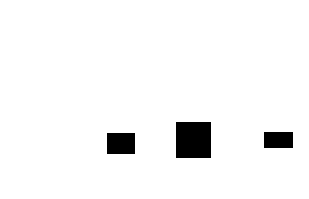
\includegraphics[width=0.4\textwidth]{afsnit/implementation/billeder/billedbehandling/binary_init}}}\hspace{1em}
    \subfloat[1. iteration]{
        \label{region1}
        \fbox{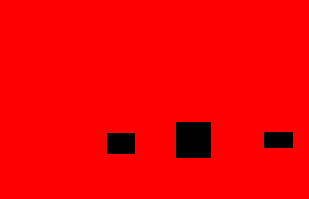
\includegraphics[width=0.4\textwidth]{afsnit/implementation/billeder/billedbehandling/binary_s1}}}\\
    \subfloat[2. iteration]{
        \label{region2}
        \fbox{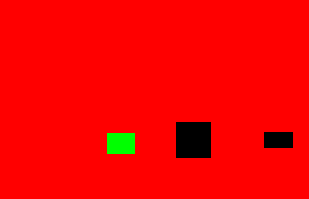
\includegraphics[width=0.4\textwidth]{afsnit/implementation/billeder/billedbehandling/binary_s2}}}\hspace{1em}
    \subfloat[3. iteration]{
        \label{region3}
        \fbox{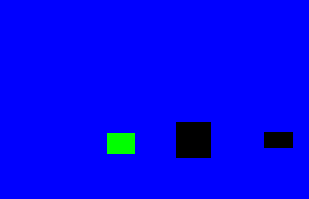
\includegraphics[width=0.4\textwidth]{afsnit/implementation/billeder/billedbehandling/binary_s3}}}\\
    \subfloat[4. iteration]{
        \label{region4}
        \fbox{\includegraphics[width=0.4\textwidth]{afsnit/implementation/billeder/billedbehandling/binary_s4}}}\hspace{1em}
    \subfloat[5. iteration]{
        \label{region5}
        \fbox{\includegraphics[width=0.4\textwidth]{afsnit/implementation/billeder/billedbehandling/binary_s5}}}\\
    \subfloat[6. iteration]{
        \label{region6}
        \fbox{\includegraphics[width=0.4\textwidth]{afsnit/implementation/billeder/billedbehandling/binary_s6}}}\hspace{1em}
    \subfloat[7. iteration]{
        \label{region7}
        \fbox{\includegraphics[width=0.4\textwidth]{afsnit/implementation/billeder/billedbehandling/binary_s7}}}
        \caption[]{Iterationerne for kodeboks \ref{naiv_segmentering}}
    \label{region_extract}
\end{figure}

Kompleksiteten stiger, når vi ikke har med binære billeder at gøre. Som
vist i kapitel \ref{chap_afproevning}, så vil vi, på grund af
tærskelværdierne til \texttt{cvFloodFill} og \texttt{cvCanny}, ikke
nødvendigvis finde de samme regioner med de to metoder. Vi ønsker at
bruge kanterne, til at indikere en ny region, så det er ikke nok, at bruge
\texttt{cvFloodFill} på midten af et linjestykke mellem kanter. I figur
\ref{floodfill_taerskel_problem} er problemet illustreret, hvor sorte
streger er detekterede kanter og lyseblå indikerer den region vi har
fundet. Hvid farve er pixels, som endnu ikke er blevet farvet af
\texttt{cvFloodFill}.  Bemærk, at linjestykket, fra kanten af billedet
til den næste detekterede kant, som krydser snittet, \emph{ikke} er
blevet farvet helt lyseblå. Dette viser, at det ikke er ligemeget på
hvilken pixel vi bruger \texttt{cvFloodFill} på linjestykker mellem
kanter. Vi ønsker derfor, at male enhver pixel, på et givet linjestykke,
som \emph{endnu ikke er blevet farvet af \texttt{cvFloodFill}}.

\begin{figure}[p]
    \setlength\fboxsep{0pt}
    \setlength\fboxrule{0.5pt}
    \centering
    \fbox{\includegraphics[width=0.8\textwidth]{afsnit/implementation/billeder/billedbehandling/floodfill_color.png}}
    \caption[]{Problemet med floodfill-metoden i billeder med flere
    farver. Hvid farve er ikke blevet malet af floodfill-metoden endnu.
    Den lyseblå region dækker ikke hele linjestykket.}
    \label{floodfill_taerskel_problem}
\end{figure}

Fremgangsmåden, for at udtrække regioner ved et snit i et arbitrært
billede, er vist i kodeboks \ref{pseudo_udtraek_org}. Metoden tager
højde for den tidligere gjorte observation, hvor en allerede fundet
region bliver overskrevet. Regioner gemmes i $\angles{CutRegions}$ på
linje 20, som opretter en ny indgang med regionens id som nøgle.
Regionens id fåes ved kaldet \texttt{color.toString()}. Ved
inspektion ses det dog, at denne fremgangsmåde lider under nøjagtig
samme svaghed som fremgangsmåden brugt i figur \ref{region_extract}.

Under udviklingen af metoden i kodeboks \ref{pseudo_udtraek_org},
opdagede vi, at det ikke altid var hele regionen der blev returneret fra
\texttt{cvFloodFill}. Vi betragter nu figur \ref{new_reg_small_box},
hvor vi har udvidet den lyseblå region fra figur
\ref{floodfill_taerskel_problem}. Regionen som bliver lagt i instansen
af \textbf{cvConnectedComp}, er den \emph{senest udfyldte}. Derfor får vi
faktisk kun returneret et undersæt, af de pixels, som udgør den lyseblå
region.

\begin{figure}[p]
    \setlength\fboxsep{0pt}
    \setlength\fboxrule{0.5pt}
    \centering
    \subfloat[En tilføjelse til den lyseblå region. Det begrænsende
    rektangel svarer kun til udvidelsen.]{
        \label{new_reg_small_box}
        \fbox{\includegraphics[angle=0,width=0.8\textwidth]{afsnit/implementation/billeder/billedbehandling/floodfill_color_new_reg_small_box}}
        }\\
    \subfloat[Ved at bruge floodfill på regionen igen, markeres hele den
    lyseblå region, som vi ønsker.]{
        \label{new_reg_big_box}
        \fbox{\includegraphics[angle=0,width=0.8\textwidth]{afsnit/implementation/billeder/billedbehandling/floodfill_color_new_reg_big_box}}
        }
    \caption[]{
    Floodfills opførsel ved udvidelse af regioner.
    }
    \label{floodfill_return_entire_region}
\end{figure}

Problemet i \ref{new_reg_small_box} løses ved at bruge
\texttt{cvFloodFill} en ekstra gang. Derfor blev kaldet til
\texttt{cvFloodFill} i linje 17 tilføjet. Man bruger derfor
\texttt{cvFloodFill} igen på den sidste pixel af linjestykket, da dette
vil returnere hele regionen, som vist i
figur \ref{new_reg_big_box}. Kaldet gør dog også, at der \emph{altid}
bliver returneret en region for hvert segment. Dette er ikke
ønskværdigt, specielt ikke hvis vi er sprunget over alle pixels på et
linjestykke. Dette sker, netop når hele regionen allerede er blevet fyldt
ud. Fejlen i linje 17 har eksisteret selv under vores kørte eksperiment
i \marker{ref}{Husk husk husk}.
Vi har fjernet duplikaterne på databaseniveau, men metoden er senere
blevet rettet til at have den korrekte opførsel. Den reviderede metode
er vist i kodeboks \ref{pseudo_udtraek_rev}.

\begin{lstlisting}[caption={Revideret pseudokode til udtrækning af
    regioner. Returnerer ingen
    duplikater.},captionpos=b,label={pseudo_udtraek_rev},numbers=left,
    frame=single, breaklines=false, float=p]
for lineSegment in Cut:
    # Get a new color that is not in the component dictionary
    color = getRandomColor()

    # Set region to None, as we have not yet found any
    region = None

    for pixel in lineSegment:

        # Check if the color of the pixel equals current color
        if not (color(pixel) ==  color):

            # Check if the color of the pixel are in the saved regions
            if not (color(pixel) in CutRegions):
                # Now we've got a new region
                region = cvConnectedComp()
                cv.cvFloodFill(img, pixel, color, lowerThres, upperThres, region)

                # Color the pixel again to make sure that
                # the returned component is the entire region
                cv.cvFloodFill(img, pixel, color, lowerThres, upperThres, region)

    # If we have found a region, then put the result in the CutRegions-dictionary
    if not (region is None):
        CutRegions[color.toString()] = (color, region)
\end{lstlisting}

Metoden i kodeboks \ref{pseudo_udtraek_rev} bruger \texttt{cvFloodFill}
to gange, hver gang man møder en ikke-farvet pixel. Dette koster lidt
køretid, men sikrer, at man altid får hele regionen returneret i
\textbf{cvConnectedComp}. Man kan fristes til at flytte kaldet i linje
21 ind i \texttt{if}-sætningen i linje 24, men dette åbner op for
svagheden igen, da vi ikke ved, om den sidste pixel tilhører den
aktuelle region. Derfor er vi nødt til at ofre lidt køretid, for at
være sikre på resultatet. Metoden benytter et ``først til
mølle''-princip, hvor en pixel, når den først et blevet tilknyttet en
region, altid vil tilhøre denne.

Pseudokoden i kodeboks \ref{pseudo_udtraek_rev} trækker dog kun de
regioner ud som rører snittet. I kapitel \ref{chap_detektion} indførtes
et margin, således at også regioner, som ligger tæt på snittet, kan
trækkes ud. Vi vil nu udvide pseudokoden i kodeboks
\ref{pseudo_udtraek_rev} til også at trække regioner ud, som krydser
margin. Vi navngiver metoden \texttt{ExtractRegions}, og den tager et
snit som argument. Metoden ses i kodeboks
\ref{pseudo_udtraek_margin}. Metoden trækker først regioner ud med
hensyn til det nedre margin, så med hensyn til det øvre margin og til
sidst med hensyn til selve snittet. Alle regioner gemmes i den samme
instans af $\angles{CutRatios}$. For selve udregningen af margin,
henvises til afsnit \ref{subsec_margin_udregning}.

\begin{lstlisting}[caption={Pseudokode til udtrækning af regioner med
    margin.},captionpos=b,label={pseudo_udtraek_margin},numbers=left,
    frame=single, breaklines=false, float=h]
def ExtractRegions(cut):
    # Calculate lowerMargin and upperMargin
    (lowerMargin, upperMargin) = calculateMargins(cut)
    Cuts = [lowerMargin, upperMargin, cut]

    # Initialize an empty CutRegions-dict
    CutRegions = {}

    for Cut in Cuts:
        for lineSegment in Cut:
            # Get a new color that is not in the component dictionary
            color = getRandomColor()

            # Set region to None, as we have not yet found any
            region = None

            for pixel in lineSegment:

                # Check if the color of the pixel equals current color
                if not (color(pixel) ==  color):

                    # Check if the color of the pixel are in the saved regions
                    if not (color(pixel) in CutRegions):
                        # Now we've got a new region
                        region = cvConnectedComp()
                        cv.cvFloodFill(img, pixel, color,
                                    lowerThres, upperThres, region)

                        # Color the pixel again to make sure that
                        # the returned component is the entire region
                        cv.cvFloodFill(img, pixel, color,
                                    lowerThres, upperThres, region)

            # If we have found a region,
            # then put the result in the CutRegions-dictionary
            if not (region is None):
                CutRegions[color.toString()] = (color, region)

    return CutRegions
\end{lstlisting}

\subsection{Svagheder\label{subsec_svagheder}}
Den endelige metode, for udtrækning af regioner, med hensyn til et givet
snit i billedet, har nogle svagheder, som bør nævnes. Den første er
allerede nævnt i den foregående sætning: Metoden trækker kun regioner ud
\emph{med hensyn} til et snit. Dette betyder, at kun regioner, som rører
margin eller selve snittet, bliver trukket ud. Foregående skal tages
helt bogstaveligt, i den forstand, at vi \emph{skal} have, at en region
har en pixel enten på det nedre margin, det øvre margin eller på selve
snittet, for at blive trukket ud. Vi kan altså godt have interessante
regioner, som faktisk har mindst én kant af sit begrænsende rektangel
inden for margin, som ikke bliver trukket ud.  Dette er tilfældet, hvis
\emph{to kanter} af det begrænsende ligger indenfor snittet, og
regionens form og størrelse i øvrigt opfylder kravene for en interessant
region. Et eksempel er vist i figur \ref{respect_to_cut}, hvor den sorte
region ikke vil blive trukket ud, selvom den har to kanter inden for
margin. Denne opførsel er beklagelig, men kan faktisk løses trivielt.
\note{Dette er måske ikke skide-smart at skrive,
men det er et vagt forsøg på at dække over egen inkompetence. Skal vi
rette koden igen?}
Det overlades som opgave til læseren, at modificere pseudokoden i
kodeboks \ref{pseudo_udtraek_margin}, så den kan udtrække regioner med
begge kanter inden for margin.
Når regioner kun trækkes ud, med hensyn til et snit, kan vi ved denne
metode heller ikke garantere en fuld segmentering af billedet.

\begin{figure}[p]
    \setlength\fboxsep{0pt}
    \setlength\fboxrule{0.5pt}
    \centering
    \fbox{\includegraphics[width=0.8\textwidth]{afsnit/implementation/billeder/billedbehandling/respect_to_cut.png}}
    \caption[]{Sort region, som ikke bliver trukket ud af billedet.
    Selvom regionens begrænsende rektangel ligger inden for margin, så
    krydser regionen hverken nedre margin, øvre margin eller selve
    snittet. Derfor opdages regionen ikke.}
    \label{respect_to_cut}
\end{figure}

\subsubsection{Valg af tilfældige RGB-værdier}
Man skal endvidere være opmærksom på, at hver gang vi markerer en ny
region, vælges en tilfældig farve til denne.  Vi kan, i vores valg af
farve, være uheldig og vælge en, som bliver brugt i det originale
billede. Når vi kalder \texttt{cvFloodFill} igen, for at være sikre, at
hele regionen bliver returneret, kan vi smelte to regioner sammen, som
egentlig ikke burde hænge sammen. I figur \ref{floodfill_colors} er
denne situation vist på det prærarerede billede fra figur \ref{bathers}.
I samme forbindelse skal vi være opmærksomme på, at vi ligeledes kan
være uheldige, at støde på en pixel, som har en farve lig med en
allerede farvet region. I dette tilfælde, vil denne pixel blive anset
som værende del af en eksisterende region, hvilket resulterer i at vi
ikke bruger \texttt{cvFloodFill} på denne. Vi kan dog håbe, at denne
pixel bliver inkluderet i den efterfølgende iteration --- hvis den næste
pixels farve, da ikke er lig en allerede udvalgt regions, og denne
ligger inden for den tilladte afvigelse, for \texttt{cvFloodFill}.  Vi
vælger aldrig, at farve en region med en farve som allerede er brugt til
en region, men vi kan også her være uheldige og vælge en farve, som
ligger inden for floodfill-metodens tilladte afvigelse.

\begin{figure}[p]
    \setlength\fboxsep{0pt}
    \setlength\fboxrule{0.5pt}
    \centering
    \subfloat[Originalt præpareret billede inden vi vælger en tilfældig
    farve til floodfill.]{
        \label{colors_1}
        \fbox{\includegraphics[width=0.3\textwidth]{afsnit/implementation/billeder/billedbehandling/pre_floodfill_1}}}\hspace{1em}
    \subfloat[Region fyldes med farve lig eksisterende pixels i
    billedet. Pixels i drengens hår har nu samme farve som kroppen.]{
        \label{colors_2}
        \fbox{\includegraphics[width=0.3\textwidth]{afsnit/implementation/billeder/billedbehandling/pre_floodfill_2}}}\\
    \subfloat[Når floodfill bruges en ekstra gang, for at være sikker på
    at hele regionen returneres, smeltes drengens krop og hår sammen.]{
        \label{colors_3}
        \fbox{\includegraphics[width=0.3\textwidth]{afsnit/implementation/billeder/billedbehandling/pre_floodfill_3}}}\hspace{1em}
    \subfloat[Hvis den første region havde fået en anden farve, ville vi
    ikke have smeltet to regioner sammen.]{
        \label{colors_4}
        \fbox{\includegraphics[width=0.3\textwidth]{afsnit/implementation/billeder/billedbehandling/pre_floodfill_4}}}\\
    \label{floodfill_colors}
    \caption[]{Uheldige valg af tilfældig farve til regioner.}
\end{figure}

\subsubsection{Ikke-sammenhængende regioner}
Metoden i kodeboks \ref{pseudo_udtraek_margin}, trækker højest én region
ud per segment. Dette giver mening, set i lyset af hvad
udtrækningsmetoden er blevet udviklet til, nemlig udtrækning af
\emph{sammenhængende regioner} afgrænset ved kantdetektion. I afsnit
\ref{section_computer_betragter} antog vi, at interessante regioner i et
billede, er tydeligt afgrænset. En region er ikke tydeligt afgrænset,
hvis vi faktisk \emph{har} flere regioner indenfor et segment. I figur
\ref{usammenhaengende_region} betragter vi en hypotetisk situation, hvor
en region ikke har været tydeligt afgrænset. Billedet i figur
\ref{usammenhaengende_region}, illustrerer et billede, som allerede er
blevet segmenteret ved metoden i kodeboks \ref{pseudo_udtraek_margin}.
De sorte cirkler markerer dér, hvor vi har fundet kanter, som krydser
snittet. Vi har altså fem segmenter på snittet. På det længste segment,
ser vi, at den mørkeblå region er blevet afbrudt af en tidligere fundet
region. Den mørkeblå region er således ikke sammenhængende. Metoden
returnerer kun den nederste mørkeblå region, da vi ikke kan få forbundet
de to mørkeblå regioner. Vi mister derfor informationen om at der
faktisk befinder sig en region i midten af billedet.

Denne opførsel, er en konsekvens af vores antagelse, om at interessante
regioner er tydeligt afgrænset. Vi accepterer derfor, at situationen i
figur \ref{usammenhaengende_region} kan forekomme, og at vi derfor kan
undlade at trække enkelte regioner ud.

\begin{figure}[t]
    \setlength\fboxsep{0pt}
    \setlength\fboxrule{0.5pt}
    \centering
    \fbox{\includegraphics[width=0.8\textwidth]{afsnit/implementation/billeder/billedbehandling/usammenhaengende_region.png}}
    \caption[]{Et segmenteret billede. Sorte cirkler angiver steder,
    hvor vi har detekteret en kant, der krydser snittet. Den mørkeblå
    region er usammenhængende over snittet, da den afbrydes af den røde
    region. Kun den nederste mørkeblå region er blevet returneret.}
    \label{usammenhaengende_region}
\end{figure}

\subsubsection{Usikkerhed ved fremhævelse af kanter}
Endeligt skal vi nævne problemerne tilknyttet måden, vi fremhæver kanter
i et billede på. Som tidligere nævnt, så fremhæves kanterne, fordi vi
har sløret billedet med en metode, som kan udviske kanterne. De
fremhævede kanter tegnes i det slørede billede med sort farve.  Sort
farve vælges, uanset hvilke farver der er brugt i maleriet. Vi kan
derfor støde på problemer med mørke malerier eller lokalt i mørke
områder af et billede. Vi kan også være uheldige, at komme til at
forbinde to regioner, ved at markere kanterne med sort.

Vi valgte, at bruge sorte kanter, da dette var den hurtigste løsning på
daværende tidspunkt. Metoden \texttt{cvFloodFill} gør det faktisk
muligt, at bruge en maske, som, i mangel af et passende dansk ord, kan
bekrives som digital malertape. Man kan kalde \texttt{cvFloodFill} med
et kantdetekteret billede, således at man ikke maler over de steder i
billedet, hvor der er detekteret en kant. \emph{OpenCV} gør det dog
yderst besværligt, at bruge denne funktion, da det kantdetekterede
billede skal være to pixel større, i hver dimension --- det
kantdetekterede billede skal have en ramme på én pixel. At indsætte en
ramme burde være trivielt, men viste sig i praksis at være meget
besværligt. En meget naiv løsning, hvor pixels kopieres én ad gangen,
var tidskrævende på store billeder og vi beholdt derfor de sorte kanter.
Alternativt kunne man beskære det originale billede, men vi besluttede
at vi ikke ville manipulere med dimensionerne på vores inddata og bevare
det originale billede.

\subsection{Andre tilgange}
Dette afsnit vil kort nævne andre fremgangsmåder, vi har prøvet, for at
trække regioner ud af et billede. Vi har tidligt i udviklingen af
programmet, eksperimenteret både med Octave og Matlab. Til at starte
med, har vi brug disse sprog til at komme problemstillingen nærmere,
og udvikle naive implementationer af enkelte algoritmer.

I præparationen af billedet, inden udtrækning af regioner, vil vi gerne
have, at farverne i billedet bliver ensartede, men vi ønsker også at
bibeholde kanterne. Vi forsøgte at bruge en metode i \emph{OpenCV} der
hedder \texttt{cvPyrMeanShiftFiltering}, som netop segmenterer billedet
efter hvilke farver der ligner hinanden, men en fejl i biblioteket
forsagede altid en segmenteringsfejl i det underliggende C-program. Vi
blev siden gjort opmærksom på en sløringsmetode af Perona og
Malik\cite{perona1990scale}, hvor det grafiske resultat tilnærmer sig
det ønskede. Kun i Octaves \emph{Image}-pakke er denne implementeret. Vi
lavede en hurtig afprøvning, hvor resultatet fra denne metode blev
analyseret, men på basis at det endelige resultat, vurderede vi, at vi
godt kunne nøjes med at fremhæve kanterne i billedet efter en simpel
sløring.

Vi har også eksperimenteret med, først at skallere billedet ned, inden
man trak regioner ud. Dette gør nemlig, at kanterne forbliver intakte,
mens farverne, til en vis grad, bliver mere ensartede. Vi stødte dog på
problemer når billedet skulle skalleres op igen, eller rettere, få
resultaterne skalleret op, så de passede til originalbilledet. Vi mister
også meget præcision, når vi bruger et nedskalleret billede til at finde
regioner i.

}

%\begin{figure}[!h]
%    \centering
%    \begin{picture}(240,30)
%        \color{black}
%        \put(0, 10){$A$}
%        \put(233, 10){$B$}
%
%        \linethickness{5mm}
%        \put(85, 0){\line(1, 0){20}}
%
%        \linethickness{9mm}
%        \put(137, 3){\line(1, 0){24}}
%
%        \linethickness{3mm}
%        \put(203, 3){\line(1, 0){21}}
%
%        \linethickness{0.2mm}
%        \put(3, -5){\line(0, 1){10}}
%
%        \put(236, -5){\line(0, 1){10}}
%
%        \put(3, 0){\line(1, 0){233}}
%    \end{picture}
%    \caption[]{Eksempel på regioner der krydser snittet.}
%    \label{impUdtraek_regioner_snit}
%\end{figure}

% vim: set tw=72 spell spelllang=da:


\section{Vurdering af regioner\label{section_vurdering_regioner}}
{
{\sffamily Vi vender nu opmærksomheden mod selve implementationen af de
metoder, som afgør, hvorvidt en udtrukket regionen er interessant, samt
hvordan vi har implementeret den naive fremgangsmåde, som bedømmer, om
en region ligger i det gyldne snit. Alle metoder vedrørende vurdering af
regioner er implementeret i filen \texttt{regionSelector.py} i mappen
\texttt{lib/}.  Vi har igen, at metoderne ikke er specifikke for det
gyldne snit, men kan anvendes på ethvert snit i billedet. Sidst i
afsnittet viser vi, hvordan vi har implementeret den udvidede vurdering.
Vi starter med at se på en fælles datastruktur, som bruges, når regioner
bliver vurderet.
}

\subsection{Datastruktur til betingelser}
Når vi skal afgøre, hvorvidt et antal udtrukne regioner er interessante
og ligger i snittet, er der en række betingelser, der skal være opfyldt.
Til disse, er der forbundet nogle udregninger, som vil være de samme for
hver region. Vi bruger derfor en struktur, som indeholder resultaterne
fra disse udregninger, således at de ikke skal udføres for hver eneste
region vi kontrollerer. Datastrukturen kaldes \textbf{Constraints} og
ses herunder i \eqref{Constraints_class}.
\begin{multline}
    \textbf{class~} \textrm{Constraints} = \{ \\
    \shoveleft{\qquad\textbf{int} : \textit{coordinate}} \\
    \shoveleft{\qquad\textbf{double} : \textit{minSize}} \\
    \shoveleft{\qquad\textbf{double} : \textit{minMass}} \\
    \shoveleft{\qquad\textbf{int[}2\delta + 1\textbf{]} : \textit{acceptRange}} \\
    \shoveleft{\}}\shoveright{}
    \label{Constraints_class}
\end{multline}
Variablene \texttt{minSize} og \texttt{minMass} relaterer sig kun til
klassificering af \emph{interessante regioner}, mens \texttt{coordinate}
og \texttt{acceptRange} hører til klassificering af regioner,
\emph{liggende i snittet}. De enkelte variable vil, i det følgende,
blive forklaret nærmere, når det er relevant.

\subsection{Interessante regioner}
Til at afgøre om udtrukket region er interessant, bruges definition
\ref{def_interessant}. Bemærk, at vurderingen af interessante regioner,
ikke har noget at gøre med hverken snitratio eller margin. Vi undersøger
udelukkende de udtrukne regioners areal og masse. Regioner bliver
vurderet, umiddelbart efter de er blevet trukket ud, så vi har
regionerne til rådighed, som en instans af $\angles{CutRegions}$. Vi
definerer nu to metoder; én til at kontrollere en regions størrelse og
én til at kontrollere dens masse. Vi kalder disse \texttt{checkSize} og
\texttt{checkMass}. De kan ses i kodeboks \ref{pseudo_size_mass}.

\begin{lstlisting}[caption={Metoder til at konstollere en regions
    størrelse og masse.},captionpos=b,label={pseudo_size_mass},
    frame=tb, breaklines=false, float]
def checkSize(component, constraints):
    "Test if the component have size greater than the minumum size
    defined by the constraints."
    return component.area >= constraints.minSize

def checkMass(component, constraints):
    "Check if the component have mass greater than the minimum mass
    defined by the contraints."
    rect = component.rect
    mass = component.area/(rect.width * rect.height)
    return mass >= constraints.minMass
\end{lstlisting}

Metoderne i kodeboks \ref{pseudo_size_mass}, returnerer begge en
sandhedsværdi, for hvorvidt en region lever op til betingelserne, for en
interessant region. Vi vil imidlertid gerne kontrollere hver enkelt
region, så vi konstruerer en ny metode, som returnerer en \emph{dict}
kun med de interessante regioner.  Metoden, kaldet
\texttt{GetInterestingRegions}, ses i kodeboks
\ref{pseudo_GetInterestingRegions}. Den tager, som argument, den instans
af $\angles{CutRegions}$, som returneres fra \texttt{ExtractRegions}, se
kodeboks \ref{pseudo_udtraek_margin}.

\begin{lstlisting}[caption={Metode som returnerer kun de insteressante
    regioner, givet en instans af $\angles{CutRegions}$}, captionpos=b,
    label={pseudo_GetInterestingRegions}, frame=tb, breaklines=false,
    float]
def GetInterestingRegions(CutRegions, constraints):
    interestingRegions = {}
    for id in CutRegions:
        component = CutRegions[id][1]
        passSizeCheck = checkSize(component, constraints)
        passMassCheck = checkMass(component, constraints)
        if (passSizeCheck and passMassCheck):
            interestingRegions[id] = CutRegions[id]
    return interestingRegions
\end{lstlisting}

I kodeboks \ref{pseudo_GetInterestingRegions} bruger vi en instans af
\textbf{Constraints} som argument til metoderne, som kontrollerer
regionens størrelse og masse. Vi skal derfor, inden metoden
\texttt{GetInterestingRegions} kaldes, have initialiseret vores
betingelser, så de passer til billedet. I kapitel
\ref{chap_afproevning}, blev fastsat en procentsats for en regions
minimumareal i forhold til billedets størrelse, og denne
minimumstørrelse findes ved udregningen i \eqref{region_min_size}
herunder.
\begin{equation}
    \mathtt{minSize} =
    \lfloor
    \mathrm{minSizePercentage}\cdot\mathrm{height}\cdot\mathrm{width}
    \rfloor
    \label{region_min_size}
\end{equation}
Ligeledes, har vi fastsat en procentsats for en regions minimummasse, men denne
skal vi ikke regne videre på, da metoden \texttt{checkMass} også regner
en procentsats ud for den givne region. Vi gemmer den fastsatte
procentsats, for regioners minimummasse direkte i vores instans af
\textbf{Constraints}. I \texttt{checkMass} sammenlignes minimummassen
med regionen masse direkte.

\clearpage
\subsection{Naiv vurdering af regioner}
Vi vil nu se på, hvordan den naive fremgangsmåde vurderer hvorvidt en
region, ligger i det gyldne snit. Definition \ref{def_naiv} siger, at en
region mindst skal have én kant inden for margin, så vi vil først give
en forklaring på, hvordan dette margin bliver repræsenteret.

\subsubsection{Udregning af margin\label{subsec_margin_udregning}}
Størrelsen på margin er givet ved en procentsats $\Delta$.  Hvis vi kun
undersøger ét snit, bliver $\Delta$ sat til $2.4\%$ af billedets højde
eller bredde, alt efter hvilken orientering det aktuelle snit har.  Vi
har implementeret fastsættelsen af $\Delta$ således, at \emph{hvis} man
ønsker at sammenligne to snit, som ligger tættere på hinanden, end det
gyldne snit og to tredjedele, så findes den værdi af $\Delta$, der gør,
at disse snits margin ikke overlapper. I praksis gives en liste med
snitratioer, der ønskes undersøgt, og fra denne liste, findes den
mindste differens mellem ratioerne. Den mindste differens mellem
snitratioer, bruges da, som $\Delta$ for alle snit i analysen. Hvis den
mindste differens, mellem snitrationerne, er større end $2.4\%$, sættes
$\Delta$ til $2.4\%$.

Når vi skal vurdere regioner med hensyn til vores margin, får vi brug
for den eksakte pixelstørrelse på margin. I filen
\texttt{marginCalculator.py} i mappen \texttt{lib/} er der implementeret
metoder til dette. Her bruges metoden \texttt{getPixels}, som, givet et
billede, et snit og $\Delta$, returnerer afstanden fra
snittet til margin i pixels, som vi også skriver som $\delta$. I
\texttt{marginCalculator.py} finder vi også den mindste differens mellem
snitratioer, ved metoden \texttt{getPercentage}.

\begin{figure}[t]
    \centering
    \begin{picture}(122,55)
        \put(61, 50){$x$}
        \put(-10, 22){$y$}
        \put(0, 45){\circle*{3}}
        \put(-1, 45){\vector(1, 0){120}}
        \put(0, 45){\vector(0, -1){48}}

        \color{red}
        \put(88, 50){\line(0, -1){55}}

        \color{blue}
        \put(84, 50){\line(0, -1){55}}
        \put(92, 50){\line(0, -1){55}}

        \color{black}

        \put(66, 30){$-^{x}$}
        \put(78, 30){\vector(1, 0){20}}

        \put(100, 30){$+^{x} $}
        \put(98, 30){\vector(-1, 0){20}}


    \end{picture}
    \caption[]{Koordinatsystem med indtegnet snit og margin. Bemærk, at
    ved det vertikale snit, skal vi kun betragte regioners $x$-værdi,
    når vi skal bedømme om de ligger inden for margin. Således kan
    margin repræsenteres kun ved de tilladte $x$-værdier.}
    \label{margin_koordinatsystem}
\end{figure}
Vi udnytter, at vi enten betragter et vertikalt eller horisontalt snit.
Når vi har et vertikalt snit, behøver vi kun at betragte $x$-værdier, da
$y$-værdien ikke influerer på det vertikale snit. Omvendt med
horisontale snit, behøver vi kun at betragte $y$-værdier, da
$x$-værdierne, i denne situation, ikke har betydning for snittet.
Tilfældet, for det vertikale snit, er vist i figur
\ref{margin_koordinatsystem}.

Ovenstående gør, at vi nu kan oprette et sæt, bestående af de
koordinater, som ligger inden for margin. Hvis vi betragter et vertikalt
snit, kan vi i Python oprette sættet af accepterende $x$-værdier, ved at
bruge \texttt{range}. Vores implementation bruger endvidere variablen
\texttt{coordinate} i \textbf{Constraints}, som, lidt misvisende,
indikerer om snittet vi undersøger, er vertikalt eller horisontalt. Er
snittet vertikalt, sættes \texttt{coordinate} til \texttt{0}, og
\texttt{1} for et horisontalt snit. For ethvert snit, kan vi da finde de
accepterende $x$-værdier, som vist i kodeboks \ref{pseudo_acceptRange}.
Variablen \texttt{margin}, der tages som argument, er den
pixelstørrelse, der er returnet fra metoden \texttt{getPixels} fra
\texttt{marginCalculator.py}.

\begin{lstlisting}[caption={Metode som genererer sættet af accepterende
    koordinater.},captionpos=b,label={pseudo_acceptRange},
    frame=tb, breaklines=false, float]
GetAcceptRange(cut, margin, coordinate):
    if coordinate:
        # Horizontal cut
        lower_bound = cut.p1.y - margin
        upper_bound = cut.p1.y + margin
        acceptRange = range(lower_bound, upper_bound)
    else:
        # Vertical cut
        lower_bound = cut.p1.x - margin
        upper_bound = cut.p1.x + margin
        acceptRange = range(lower_bound, upper_bound)

    return acceptRange
\end{lstlisting}

\subsubsection{Kontrol på en regions begrænsende rektangel}
\begin{lstlisting}[caption={Metode, som kontrollerer, hvorvidt en region
    har en kant af det begrænsende rektangel inden for margin.},
    captionpos=b, label={pseudo_position}, frame=tb, breaklines=false,
    float]
def checkPosition(component, constraints):
    "Test if the component have a bounding box inside the accepting
    rectangle defined in the constraints."
    d = component.rect.width
    p = component.rect.x
    if constraints.coordinate:
        d = component.rect.height
        p = component.rect.y

    lowerInRange = p in constraints.acceptRange
    upperInRange = (p + d) in constraints.acceptRange

    return lowerInRange or upperInRange
\end{lstlisting}
Når vi har fastsat \texttt{coordinate} og fundet værdierne i
\texttt{acceptRange} kan vi kan afgøre, om en interessant region, ligger
placeret i snittet. Vi har allerede udnyttet, at vi kun behøver at
betragte én koordinat, og det er derfor ligetil, at kontrollere, om en
regions begrænsende rektangel, har en kant inden for margin. Regionen er
repræsenteret som en instans af \textbf{cvConnectedComp}, hvori der er
en instans af \textbf{cvRect}. Vi har en metode, kaldet
\texttt{checkPosition}, som, alt efter om vi har et vertikalt eller et
horisontalt snit, returnerer en sandhedsværdi for, om den relevante
koordinat findes i de accepterende koordinater. Metoden ses i kodeboks
\ref{pseudo_position}.

Vi kan nu sammensætte en metode, som returnerer alle interessante
regioner, med en kant inden for margin. Metoden tager en instans af
$\angles{CutRegions}$ og en instans af \textbf{Constraints} som
argumenter. Vi genererer altså vores betingelser inden vi begynder at
frasortere regioner, således at alle informationer om snittet og krav
for regioner ligger i instansen af \textbf{Constraints}. Den endelige
metode, for vurdering efter den naive fremgangsmåde, kaldes
\texttt{GetInterestingRegionsInCut} og er vist i kodeboks
\ref{pseudo_GetInterestingRegionsInCut}.

\begin{lstlisting}[caption={Pseudokode, som returnerer alle interessante
    regioner, der har en kant, af deres begrænsende rektangel, inden for
    margin.},
    captionpos=b, label={pseudo_GetInterestingRegionsInCut}, frame=tb, breaklines=false,
    float]
def GetInterestingRegionsInCut(CutRegions, constraints):

    # First remove uninteresting regions
    interestingRegions = GetInterestingRegions(CutRegions, constraints)

    # Initialize an empty dict
    interestingRegionsInCut = {}

    # Check every interesting region if it's bounding box
    # has an edge inside the margin
    for id in interestingRegions:
        component = interestingRegions[id][1]
        if checkPosition(component, constraints):
            interestingRegionsInCut[id] = interestingRegions[id]

    # The resulting dict contains only interesting regions
    # with an edge inside the margin
    return interestingRegionsInCut
\end{lstlisting}

\subsection{Udvidet vurdering af regioner}
Vi har også implementeret en udvidet vurdering af interessante
regioner. Grundprincipperne bag denne er gennemgået i afsnit
\ref{subsec_udvidet_massemidtpunkt}. Da vi ikke længere betragter en
regions begrænsende rektangel, men i stedet regionens form og
udstrækning, har brug vi for en anden måde, at repræsentere regionen på.
Vi tager derfor billedet, som \texttt{cvFloodFill} har arbejdet på, og
bruger dette til at approksimere regionens form.

\subsubsection{Approksimation af regioners form og udstrækning}
Fremgangsmåden for at approksimere en regions form og udstrækning er
simpel. Givet et segmenteret billede, fra \texttt{cvFloodFill}, og den
resulterende $\angles{CutRegions}$, fra \texttt{ExtractRegions}, kan vi,
for hver pixel i det begrænsende rektangel, kontrollere om denne har
samme farve, som regionen er blevet tildelt i segmentering af billedet.
Hvis farverne er ens, så gemmes dette punkt i en liste. Hvis regionen er
stor, kan dette godt være en tidskrævende procedure, så i praksis ønsker
vi ikke at kontrollere hver eneste pixel i det begrænsende rektangel. Vi
springer derfor et antal pixels over, for hver gang vi har kontrolleret
en pixel.  På denne måde får vi lavet et gitter, som vist i figur
\ref{grid}.  Pseudokode, for at approksimere en regions form og
udstrækning, er vist i kodeboks \ref{pseudo_GetRegionGrid}, som
definerer metoden \texttt{GetRegionGrid}, der returnerer en liste med
punkter for en region.

\begin{lstlisting}[caption={Metode til at approksimere en regions
    form. Bemærk linje 19, hvor der ses et eksempel på det omvendte
    koordinatsystem i \emph{OpenCV}.}, captionpos=b,
    label={pseudo_GetRegionGrid}, frame=tb,
    breaklines=false, float, numbers=left]
def GetRegionGrid(image, color, component, step):
    rect = component.rect

    # Initialize the area we want to traverse
    lower_x = rect.x
    lower_y = rect.y
    upper_x = lower_x + rect.width
    upper_y = lower_y + rect.height

    # Initialize an empty array
    coordinates = []

    # Traverse the bounding box with the defined step size
    for x in range(lower_x, upper_x, step):
        for y in range(lower_y, upper_y, step):

            # If we find a color in the image that equals the region
            # color, then we save that point
            if isSameColor(color, image[y][x]):
                coordinates.append(cvPoint(x, y))

    # Finally, return the resulting set of points
    return coordinates
\end{lstlisting}
% Sorry, I'm really sorry :(
Til senere brug, vil vi definere en metode, som finder en approksimation
til alle regioner i en instans af $\angles{CutRegions}$. Denne metode
returnerer en modificeret instans af $\angles{CutRegions}$, som vi
kalder for $\angles{CutGridRegions}$, således at den også indeholder
approksimationen til regionen. Strukturen er vist i
\eqref{CutGridRegions_dict}.
\begin{multline}
    \angles{CutRegions} = \{ \textit{~RegionId} : \\
    (\textbf{CV\_RGB~}\textit{color}, \textbf{cvConnectedComp~}\textit{region}, \textbf{cvPoint[]~}\textit{grid}) \}\quad
    \label{CutGridRegions_dict}
\end{multline}
Metoden \texttt{GridIt}, er vist i kodeboks \ref{pseudo_GridIt}, og går
alle regionerne igennem, mens den bygger den nye \emph{dict} op.

\begin{lstlisting}[caption={Metode, som finder approksimationen til alle
    regioner i en instans af $\angles{CutRegions}$.}, captionpos=b,
    label={pseudo_GridIt}, frame=tb,
    breaklines=false, float]
def GridIt(image, CutRegions, step):
    # Initialize an empty dict
    CutGridRegions = {}

    for id in CutRegions:
        # Get the color and component
        color = CutRegions[id][0]
        component = CutRegions[id][1]

        # Get the grid for the region
        grid = GetRegionGrid(image, color, component, step)

        # Save the findings
        CutGridRegions[id] = (color, component, grid)

    # Well, return
    return CutGridRegions
\end{lstlisting}

\subsubsection{Vurdering ved massemidtpunkt og udstrækning}
Definition \ref{def_expanded} fortæller os, at hvis en region har et
massemidtpunkt inden for margin og dens masse i øvrigt er jævnt fordelt
over snittet, så ligger denne i snittet.  En regions fordeling af masse
er givet i definition \ref{def_fordeling_ligning} og en regions
massemidtpunkt er givet i definition \ref{def_massemidtpunkt}. Vi skal
bruge approkimationen af regionens form og udstrækning til at afgøre om
regionen ligger i snittet.

Vi starter med at kigge på fordelingen af en regions masse, hvor vi skal
finde forholdet mellem punkter på højre og venstre side af snittet.
Metoden i kodeboks \ref{pseudo_distribution}, gør netop dette, og
returnerer en sandhedsværdi for, om regionens masse er jævnt fordelt
over snittet. Definition \ref{def_fordeling_procent} siger, at regionens
masse er jævnt fordelt over et snit, hvis forholdet mellem de to sider
er under $0.75$.  Metoden gør brug af snittets orientering, hentet i
$\textbf{Constraints}.\textit{coordinate}$, og det faktum, at vi kan
finde det midterste element i vores accepterende værdier, ved at tage
det $\left(\left\lfloor \frac{|\textit{acceptRange}|}{2}\right\rfloor +
1\right)$'te element i $\textbf{Constraints}.\textit{acceptRange}$.
Dette er selve snittet.

\begin{lstlisting}[caption={Metode som, på baggrund af regionens
    fordeling af masse, afgør, om denne region er jævnt fordelt},
    captionpos=b, label={pseudo_distribution}, frame=tb,
    breaklines=false, float]
def checkDistribution(grid, constraints):
    # If we've got no approximation, there's no distribution
    if len(grid) == 0:
        return False

    # Init variables for right/left-distribution as floats
    rDist = 0.0
    lDist = 0.0

    # Get the middle value of the accepting range, i.e. the cut
    middleIndex = floor(len(constraints.acceptRange)/2) + 1
    cutVal = constraints.acceptRange[middleIndex]

    # Check the position of every pixel in the grid
    for point in grid:
        if constraints.coordinate:
            # Horisontal
            if cutVal > point.y:
                left += 1
            elif cutVal < point.y:
                right += 1
        else:
            # Vertical
            if cutVal > point.x:
                left += 1
            elif cutVal < point.x:
                right += 1

    distribution = abs((lDist - rDist)/len(grid))
    return distribution < 0.75
\end{lstlisting}

Vi skal også bruge en metode, til at finde en regions massemidtpunkt.
Denne metode er vist i kodeboks \ref{pseudo_checkCenterOfMass} og
returnerer en sandhedsværdi for, hvorvidt en regions massemidtpunkt
befinder sig inden for margin.

\begin{lstlisting}[caption={Metode, som kontrollerer, om en regions
    massemidtpunkt er inden for margin.}, captionpos=b,
    label={pseudo_checkCenterOfMass}, frame=tb, breaklines=false,
    float]
def checkCenterOfMass(grid, constraints):
    if len(grid) == 0:
        return False

    sum = 0
    for point in grid:
        if constraints.coordinate:
            # Horisontal
            sum += point.y
        else:
            # Vertical
            sum += point.x

    centerOfMass = sum/len(grid)

    return centerOfMass in constraints.acceptRange
\end{lstlisting}

Endeligt samler vi alle metoderne, så vi kan sortere i alle resultaterne
returneret fra segmentering af billedet. Vi kalder denne metode for
\texttt{GetExpandedRegions} og viser denne i kodeboks
\ref{pseudo_GetExpandedRegions}.

\begin{lstlisting}[caption={Pseudokode, som returnerer alle interessante
    regioner, der er nævnt fordelt over snittet og har et massemidtpunkt
    inden for margin.},
    captionpos=b, label={pseudo_GetExpandedRegions}, frame=tb, breaklines=false,
    float]
def GetExpandedRegions(image, CutRegions, constraints):

    # First remove uninteresting regions
    interestingRegions = GetInterestingRegions(CutRegions, constraints)

    # Initialize the grid
    interestingRegions = GridIt(image, interestingRegions, constraints)

    # Initialize an empty dict
    interestingRegionsInCut = {}

    # Check every interesting region for center of mass
    # and distribution
    for id in interestingRegions:
        grid = interestingRegions[id][2]
        if checkDistribution(grid, constraints)
            and checkCenterOfMass(grid, constraints):
            interestingRegionsInCut[id] = interestingRegions[id]

    # The resulting dict contains only interesting regions
    # that qualify
    return interestingRegionsInCut
\end{lstlisting}

\clearpage

}

% vim: set tw=72 spell spelllang=da:


\section{Database\label{section_imp_database}}
{
Når vi har trukket regioner ud af billedet og vurderet dem efter
ovenstående simple algoritme kan vi stå tilbage med et egentligt
resultat. Vi ønsker at gemme dette resultat i en database så vi på et
senere tidspunkt kan bruge det i en samlet analyse af resultaterne.
Vi så i afsnit \ref{section_opbv_billeder} på et databaseskema til
opbevaring af maleriers metadata. Vi bygger nu videre på dette skema så
vi kan tilknytte resultater fra en analyse til de enkelte malerier. Det
fulde databaseskema ses nedenfor.

\begin{table}[!h]
    \centering
    \begin{tabular}{|l||c|c|c|c|c|c|}
        \hline
        \bf{artist} \hspace{0.5cm} & \underline{artistId} & name & born & died & school & timeline \\\hline
    \end{tabular}
    \caption{Databasetabel for kunstner}
    \label{artistTable}
\end{table}

\begin{table}[!h]
    \centering
    \begin{tabular}{|l||c|c|c|c|c|c}
        \hline
        \bf{painting} \hspace{0.5cm} & \underline{paintingId} & artistId & title & date & paint & $\cdots$ \\\hline
    \end{tabular}\\ \vspace{0.2cm}\hspace{1.2cm}
    \begin{tabular}{c|c|c|c|c|c|c}
        \hline
        $\cdots$ & material & location & url & form & type & $\cdots$ \\\hline
    \end{tabular}\\ \vspace{0.2cm}\hspace{1.4cm}
    \begin{tabular}{c|c|c|c|c|c|}
        \hline
        $\cdots$ & realHeight & realWidth & height & width & filepath \\\hline
    \end{tabular}
    \caption{Databasetabel for malerier}
    \label{paintingTable}
\end{table}

\begin{table}[!h]
    \centering
    \begin{tabular}{|l||c|c|c|c|c|c|c|}
        \hline
        \bf{run} \hspace{0.5cm} & \underline{runId} & trsh1 & trsh2 & lo & up & marginPercentage & method \\\hline
    \end{tabular}
    \caption{Databasetabel for en kørsel}
    \label{runTable}
\end{table}

\begin{table}[!h]
    \centering
    \begin{tabular}{|l||c|c|c|c|c|c|}
        \hline
        \bf{result} \hspace{0.5cm} & \underline{resultId} & runId & paintingId & cutRatio & cutNo & numberOfRegions \\\hline
    \end{tabular}
    \caption{Databasetabel for resultater}
    \label{resultTable}
\end{table}

\begin{table}[!h]
    \centering
    \begin{tabular}{|l||c|c|c|c|c|c|c|}
        \hline
        \bf{region} \hspace{0.5cm} & \underline{regionId} & resultId & x & y & height & width & area \\\hline
    \end{tabular}
    \caption{Databasetabel for regioner}
    \label{regionTable}
\end{table}

Tabellerne \ref{artistTable} og \ref{paintingTable} er de samme som vist
i afsnit \ref{section_opbv_billeder}, men er taget med her blot for at
vise databaseskemaet i sin helhed. Det øvrige databaseskema lægger vægt
på at minimere redundans og mulighed for at genskabe kørte analyser.
Sidstnævnte er vigtig osv\dots

}
% vim: set tw=72 spell spelllang=da:


\section{Kørsel\label{section_koersel}}
\textbf{Sæt sammen med database-afsnittet}\\
Flow diagram (flot).
\subsection{Indstillinger}
Snak om indstillinger for de enkelte kørsler og globale indstillinger.

}

% vim: set tw=72 spell spelllang=da:


\chapter{Videnskabelige resultater\label{chap_resultater}}
{
{\sffamily Vi vil i dette kapitel se på, hvilke resultater, vi med vores
metoder, er kommet frem til. Vi præsenterer en række hypoteser og
undersøger hvorvidt vores data kan be- eller afkræfte disse hypoteser.
Vi vil også gerne se, om vores data fremvise nogle interessante
observationer vedrørende kunstneres oprindelse eller fødselsår.
}

\section{Hypoteser}
{
{\sffamily Vi vil i det følgende præsentere de hypoteser, som vi, på
baggrund af resultaterne af den efterfølgende analyse på vores datasæt,
vil forsøge at verificere. De fleste af hypoteserne antager den
generelle opfattelse, at det gyldne snit er specielt æstetisk tiltalende
og af denne grund, er meget brugt i malerkunsten. Sidst i afsnittet vil
vi kaste et kritisk blik på vores datasæt, for at se på hvad vi kan
forvente af vores analyse.
}

\begin{hypotese}
    Hvis det gyldne snit er meget brugt i malerkunsten, må vi have, at
    over halvdelen, af de analyserede malerier, har én eller flere
    regioner liggende i det gyldne snit.
\end{hypotese}

\emph{eller}

\begin{hypotese}
    I en analyse på et stort antal malerier, vil over halvdelen af disse
    have mindst én region i det gyldne snit, da det gyldne snit bliver
    brugt meget i malerkunsten.
\end{hypotese}

\emph{eller}

\begin{hypotese}
    Det gyldne snit er meget brugt i malerkunsten, da over halvdelen, af
    de analyserede malerier, har én eller flere regioner liggende i det
    gyldne snit.
    \label{hypo_binaer}
\end{hypotese}

\hrule

\begin{hypotese}
    Hvis et gyldent snit er specielt æstetisk tiltalende, må vi have, at
    antallet af regioner liggende hvert af de fire snit, som kan
    betragtes som gyldne, ikke afviger mere end $\pm10\%$ fra hinanden.
\end{hypotese}

\emph{eller}

\begin{hypotese}
    Et gyldent snit er specielt æstetisk tiltalende, da antallet af
    regioner, liggende i hvert af de fire gyldne snit, ikke afviger med
    mere end $\pm10\%$ fra hinanden.
\end{hypotese}

\hrule

\begin{hypotese}
    Hvis det gyldne rektangel er et specielt æstetisk tiltalende format,
    må vi have, at mere end en tredjedel malerierne har et lærred, hvis
    dimensioner er lig $\varphi\pm2.4\%$.
\end{hypotese}

\emph{eller}

\begin{hypotese}
    Det gyldne rektangel er et specielt æstetisk tiltalende format,
    fordi mere end en tredjedel af alle malerier, har et lærred, hvor
    forholdet mellem dimensionerne  er lig $\varphi\pm2.4\%$.
\end{hypotese}

\hrule

\begin{hypotese}
    Hvis det gyldne snit er bevidst brugt af kunstneren, må vi have, at
    antallet regioner liggende i det gyldne snit, er skarpt større, end
    antallet af regioner liggende i snittet ved to tredjedele.
    \label{hypo_golden_ractangle}
\end{hypotese}

\emph{eller}

\begin{hypotese}
    Det gyldne snit bruges bevidst af kunstnere, da der findes flere
    regioner i det gyldne snit, end i snittet ved to tredjedele.
	\label{hypototredjedele}
\end{hypotese}

\hrule

\begin{hypotese}
    Hvis det gyldne snit er meget brug i malerkunsten, må vi have, at
    antallet af detekterede regioner i det gyldne snit, er skarpt
    større, end antallet i alle andre snit.
\end{hypotese}

\emph{eller}

\begin{hypotese}
    Det gyldne snit er meget brugt i malerkunsten, fordi der findes
    flere regioner i det gyldne snit end antallet af regioner liggende i
    ethvert andet snit.
	\label{hypoethvertandetsnit}
\end{hypotese}

\hrule

\begin{hypotese}
    Hvis det gyldne snit er bevidst brugt af kunstneren, må vi have, at
    antallet regioner liggende i det gyldne snit, er skarpt større, end
    antallet af regioner liggende det midterste snit.
\end{hypotese}

\emph{eller}

\begin{hypotese}
    Det gyldne snit bruges bevidst af kunstnere, da der findes flere
    regioner liggende i det gyldne snit end antallet af regioner
    liggende i det midterste snit.
	\label{hypomidten}
\end{hypotese}

\hrule

\begin{hypotese}
    Hvis det gyldne snit altid har været specielt æstetisk tiltalende,
    må vi have, at antallet af regioner liggende i det gyldne snit,
    tidsperioder imellem, højest kan afvige med $\pm10\%$.
\end{hypotese}

\emph{eller}

\begin{hypotese}
    Det gyldne snit har altid været lige meget brugt i malerkunsten, fordi
    antallet af regioner i det gyldne snit, tidsperioder imellem, kun
    afviger med $\pm10\%$.
\end{hypotese}

\hrule

\begin{hypotese}
    Hvis det gyldne snit er ligeså  æstetisk tiltalende for alle,
    må vi have, at antallet af regioner liggende i det gyldne snit,
    nationaliteter imellem, højest kan afvige med $\pm10\%$.
\end{hypotese}

\emph{eller}

\begin{hypotese}
    Det gyldne snit er lige æstetisk tiltalende for alle, fordi antallet
    af regioner liggende i det gyldne snit, nationaliteter imellem, kun
    afviger med $\pm10\%$.
\end{hypotese}

\hrule

\begin{hypotese}
    Hvis det gyldne snit er specielt æstetisk tiltalende, og vi har at
    \emph{the rule of thirds} bliver brugt i malerkunsten, som en
    approksimation til det gyldne snit, må vi have, at antallet af
    regioner liggende i det gyldne snit ikke angiver fra antallet af
    regioner i to tredjedele med mere end $15\%$.
\end{hypotese}

\emph{eller}

\begin{hypotese}
    \emph{The Rule of Thirds} bliver brugt i malerkunsten som en
    approksimation til det gyldne snit, fordi antallet af regioner, som
    findes i det gyldne snit, ikke afviger med mere end $\pm15\%$ fra
    antallet af regioner, som findes i snittet ved to tredjedele.
\end{hypotese}

\subsection{Datasæt}
Det korpus, vi kører vores analyse på, består af billeder hentet fra
``The Web Gallery of Art''\cite{wgahu}, som er en online billededatabase, med
europæiske kunstartikler fra år 1001 -- 1900. I kunstartiklerne, hvor
det samlede antal er omkring 23.000, indgår møbler, kalkmalerier,
skulpturer, mosaikker og malerier, hvor sidstnævnte, vil være vores
fokus. Over halvdelen af disse kunstartikler står udstillet på museum.
Databasen blev oprettet i 1996, med det formål at præsentere kunst fra
renæssancen (ca.  14. -- 17.  århundrede), men blev senere udvidet, til
også at inkludere kunst fra andre perioder. Dette betyder, at
størstedelen af malerierne vi undersøger, er fra tidsperioden 1450 --
1650 og er malet af italienske kunstnere. Endvidere er langt de fleste
malerier, klassificeret som religiøse.  Disse informationer er givet fra
WGA, men er også suppleret i bilag \ref{appendix_grafer} som
grafer.

Vi må af ovenstående grunde forvente, at resultater, fra en analyse på
vores datasæt, vil være farvet af samlingen af malerier, og det derfor
kan være svært at drage nogen konklusioner for malerkunsten generelt, da
resultaterne vil være begrænset, til kun at gælde for et udsnit af
vestlig kultur. Endvidere findes der ingen nyere malerier i datasættet,
hvilket gør at vi ikke kan udtale os om nyere malerkunst.

Billederne, som suppleres fra databasen, er af høj kvalitet, men der er
visse problemer, som vi nævner nedenfor.

\begin{itemize}
    \item \textbf{Beskæring af billeder}\\
        Vi kan ikke vide os sikre på, om billederne i datasættet er
        ordentligt beskåret, hvilket betyder at vi \emph{kan} have, at
        noget af billedrammen er med i billedet. Dette kan muligvis
        volde lidt problemer med udtrækning af regioner, men hvad værre
        er, så gør det vores mål, for hvor det gyldne snit ligger,
        upræcist. Dette har vi dog taget højde for, i kraft af vores
        margin.  Endeligt er der inkluderet billeder af malerier
        detaljer i databasen, som er udsnit af maleriet, således at
        målene på billedet ikke passer.
    \item \textbf{Forvrængning og perspektiv}\\
        Billederne af malerier er taget med et kamera, hvor linsen muligvis kan
        forvrænge billedet. Vi kan derfor have skæve linjer og tage
        forkerte beslutninger, for regioner, pga. dette. Endvidere kan
        billedet være taget skævt, således at billedet hælder til den
        ene side. Vi kan selvfølgelig også have at perspektivet i
        billedet er forkert, fordi billedet er taget fra en skæv vinkel.
    \item \textbf{Opdelte malerier}\\
        Nogle store malerier kan være blevet opdelt, da databasen har
        det formål at vise malerierne på en computerskærm, hvor meget
        store billeder kan være svære at betragte. Dette betyder, at
        nogle billeder ikke viser hele maleriet, men blot er et udsnit,
        hvilket påvirker vores muligheder for at sige noget fornuftigt
        om det gyldne snit i maleriet.
\end{itemize}

Nogle stilarter, såsom kalkmalerier og tegninger, har gennem
udokumenterede afprøvninger, vist sig at være besværlige at analysere,
pga. meget svingende farvegengivelse. Endvidere, kan disse være billeder
af en hvælving i en kirke, som ikke egner sig til analyse for det gyldne
snit. Vi har derfor valgt kun at analysere malerier, kendetegnet ved at
de er beskrevet som ``painting'' fra WGA.

Alt det ovenstående vil påvirke resultaterne, ved analyse på vores
datasæt.

}
% vim: set tw=72 spell spelllang=da:


\section{Naiv implementation\label{section_naiv_koersel}}
{
{\sffamily I det følgende vil vi samle op på resultaterne fra det kørte
eksperiment med den naive vurdering af regioner. Vores metode til
udtrækning af regioner, har dog indeholdt en fejl, som vi først vil
beskrive.
}

\subsection{Systematisk fejl\label{program_bug}}
I den naive løsning findes en fejl i udtrækningen af regioner, som gør
at vi finder nogle af
regionerne flere gange. Denne fejl nævnt i afsnit
\ref{section_impBilledbehandling} og gennemgået i bilag
\ref{appendix_bug}. Det betyder, at de resultater vi fremviser for kørslen
af den naive løsning, ikke helt passer. For at give en indblik i, hvor
mange regioner der bliver fundet flere gange, har vi afprøvet programmet med
fejlen på 11 malerier, og sammenlignet dem med en kørsel, hvor fejlen er
rettet.

De 11 malerier er opstillet i tabel \ref{bug_tabel}, hvor de to første
kolonner er antal regioner fundet i billedet, uden og med fejl.  Tredje
kolonne er en procentsats for, hvor mange flere regioner der bliver
fundet, når den fejlende kode køres. Den procentvise spredning er $[60
\%,~377 \%]$, så de resultater vi får, kan være op til $377\%$ for høje.
Gennemsnitligt er der $172 \%$ flere regioner. Vi kan godt antage, at
antallet af regioner opgivet i resultaterne for den naive løsning, er
halv så store.

\begin{table}[!h]
    \centering
    \begin{tabular}{|l|c|c|c|}
        \hline
  Maleri  & Bug løst 		& Bug ikke løst		& Procentvis forskel\\\hline
        1   & 70 			& 112 				& 60 \% \\
        2   & 27 			& 45 				& 67 \% \\
        3	& 52 			& 98 				& 72 \% \\
        4   & 84 			& 145 				& 73 \% \\
        5	& 32 			& 57 				& 78 \% \\
        6   & 88 			& 170 				& 93 \% \\
        7   & 85 			& 201 				& 136 \% \\
        8   & 78 			& 197 				& 153 \% \\
        9   & 164 			& 554 				& 238 \% \\
        10	& 16 			& 75 				& 368 \% \\
        11	& 115 			& 548 				& 377 \% \\\hline
	Total	& 881			& 2202				& 172 \% \\\hline
	  \end{tabular}
    \caption[]{Tabel for antal fundne regioner i versionen med og uden
    fejlen som duplikerer regioner. Den sidste kolonne er hvor mange
    procent flere regioner der bliver fundet.}
    \label{bug_tabel}
\end{table}

\clearpage

\subsection{Resultater}
Vi har kørt analyse med naiv vurdering på $17,364$ malerier, men i vores
resultater sorterer vi $2,989$ af disse fra, da de kun er udsnit af et
større maleri.  Som vist i tabel \ref{tabel_fjern_detaljer} herunder, er
dette en nedgang på $17.21$ procent og vi har $14,375$ brugbare
resultater tilbage.

\begin{table}[H]
    \centering
    \begin{tabular}{r@{\ \ }p{12em}r|r@{.}l}
            & Analyserede malerier & $17,364$ & $100$ & $00\%$   \\
        $-$ & Udsnit af malerier   &  $2,989$ &  $17$ & $21\%$   \\\hline
            & Resultater           & $14,375$ &  $82$ & $79\%$
    \end{tabular}
    \caption[]{Udregning af brugbare resultater.}
    \label{tabel_fjern_detaljer}
\end{table}

Af de brugbare resultater, ser vi i tabel \ref{tabel_fordeling}, at der
i $91.43$ procent af malerierne er fundet mindst én region som ligger i
det gyldne snit. Vi kan derfor ikke afvise hypotese \ref{hypo_binaer}.

\begin{table}[H]
    \centering
    \begin{tabular}{r@{\ \ }p{12em}r|r@{.}l}
            & Positive resultater   & $13,143$ &  $91$ & $43\%$ \\
        $+$ & Negative resultater   &  $1,232$ &   $8$ & $57\%$ \\\hline
            & Resultater i alt      & $14,375$ & $100$ & $00\%$
    \end{tabular}
    \caption[]{Et positivt resultat beskriver et maleri, hvori der er
    fundet mindst én region, som ligger i det gyldne snit. Et negativt
    resultat er et maleri, hvori der ikke findes nogen regioner, som
    ligger i det gyldne snit.}
    \label{tabel_fordeling}
\end{table}

Vi vil gerne se på, hvordan fordelingen af fundne interessante regioner i
de fire gyldne snit ser ud. Fordelingen er vist i tabel
\ref{tabel_fire_snit}. Vi ser, at ingen af snittene afviger med mere end
$\pm10\%$ fra et andet og vi kan derfor ikke afvise hypotese
\ref{hypo_fire_g_snit}.

\begin{table}[H]
    \centering
    \begin{tabular}{r@{\ \ }p{12em}r|r@{.}l}
            & Regioner i snit 0   &  $42,884$ &  $24$ & $51\%$ \\
        $+$ & Regioner i snit 1   &  $44,042$ &  $25$ & $18\%$ \\
        $+$ & Regioner i snit 2   &  $46,432$ &  $26$ & $54\%$ \\
        $+$ & Regioner i snit 3   &  $41,547$ &  $23$ & $75\%$ \\\hline
            & Regioner i alt      & $168,650$ & $100$ & $00\%$
    \end{tabular}
    \caption[]{Forholdet mellem de interessante regioner fundet i de
    fire gyldne snit. Intet snit afviger med mere end $10\%$ fundne
    regioner, end et andet snit.}
    \label{tabel_fire_snit}
\end{table}

Vi undersøger nu, hvor mange af de brugbare resultater, som er forsynet
med dimensioner i databasen, således at vi kan undersøge, hvorvidt
lærredet er konstrueret som et gyldent rektangel. Udregningen i tabel
\ref{tabel_med_dimensioner} viser at ud af de brugbare resultater,
mangler $2,410$ malerier dimensionerne, og vi har da $11,965$ malerier
tilbage at undersøge, for den gyldne ratio i lærredets dimensioner.

\begin{table}[H]
    \centering
    \begin{tabular}{r@{\ \ }p{14em}r|r@{.}l}
            & Resultater                     & $14,375$ & $100$ & $00\%$ \\
        $-$ & Resultater uden dimensioner    &  $2,410$ &  $16$ & $77\%$ \\\hline
            & Resultater med dimensioner     & $11,965$ &  $83$ & $23\%$
    \end{tabular}
    \caption[]{Brugbare resultater med dimensioner i databasen.}
    \label{tabel_med_dimensioner}
\end{table}

Vi ser nu, hvor mange af de $11,965$ malerier, der har, at dets lange
side, $L$, divideret med dets korte side, $K$, ligger i intervallet $G =
[1.57920117302, 1.65686680448] = \varphi \pm 2.4\%$. Tabel
\ref{tabel_real_dimensions} viser, at kun $3.99\%$ falder inden for
dette interval. Vi kan således afvise hypotese
\ref{hypo_golden_ractangle}.

\begin{table}[H]
    \centering
    \begin{tabular}{r@{\ \ }p{14em}r|r@{.}l}
            & $L/K \in G$                  &    $478$ &   $3$ & $99\%$ \\
        $+$ & $L/K \notin G$               & $11,487$ &  $96$ & $01\%$ \\\hline
            & Resultater med dimensioner   & $11,965$ & $100$ & $00\%$
    \end{tabular}
    \caption[]{Resultater med dimensioner, hvor disse er et gyldent
    rektangel med en afvigelse på $2.4\%$. Under en tredjedel af
    malerierne har et lærred med gyldne dimensioner.}
    \label{tabel_real_dimensions}
\end{table}

\begin{table}[H]
    \centering
    \begin{tabular}{|c|l|c|c|}
		\hline
        \textbf{Hypotese nr.} & \textbf{Beskrivelse} & \textbf{Afvist} &
        \textbf{Ikke afvist}  \\\hline\hline
        1 & Mindst én region i $GS$                     &            & \checkmark   \\\hline
        2 & Alle fire $GS$ lige meget brugt             &            & \checkmark   \\\hline
        3 & $1/3$ har lærred med forholdet $1:\varphi $ & \checkmark &              \\\hline
        4 & Flest regioner i $GS$                       & \checkmark &              \\\hline
        5 & Flere regioner i $GS$ end $\frac{2}{3}$     &            & \checkmark   \\\hline
        6 & Flere regioner i $GS$ end i midten          & \checkmark &              \\\hline
        7 & $GS$ brugt lige meget, uanset tidsperiode   & \checkmark &              \\\hline
        8 & $GS$ brugt lige meget, uanset nationalitet  & \checkmark &              \\\hline
        9 & $\frac{2}{3}$ brugt som approksimation til $GS$   &            & \checkmark	\\\hline
    \end{tabular}
    \caption[]{Hypoteser i forhold til den naive kørsel. $GS$ bruges som
    forkortelse for det gyldne snit.}
    \label{hypoteser_naiv}
\end{table}

\subsubsection{Antallet af fundne regioner over alle snit}
I alle $14,375$ malerier er der i alt fundet $1,650,082$ interessante
regioner. Vi har en middelværdi på $114.79$ med standardafvigelse på
$86.91$. I figur \ref{total_regions_plots} er vist grafer over hvordan
antallet af fundne regioner fordeler sig i malerierne. I figur
\ref{graf_total_regions_zoom}, hvor der ses bort fra $298$ malerier,
hvori der ikke er fundet nogen regioner. Regionerne i malerierne har en
fordeling, der kunne ligne en eksponentialfordeling, som vist i
histogrammet i figur \ref{hist_total_regions}. De observerede værdier
fraviger dog noget fra de teoretiske værdier.

\begin{figure}[!h]
    \centering
    \subfloat[]{
        \includegraphics[width=0.49\textwidth]{afsnit/resultater/billeder/totalregions_var}
        \label{graf_total_regions_var}
    }
    \subfloat[]{
        \includegraphics[width=0.49\textwidth]{afsnit/resultater/billeder/totalregions}
        \label{graf_total_regions_zoom}
    }\\
    \subfloat[]{
        \includegraphics[width=0.62\textwidth]{afsnit/resultater/billeder/hist_totalregions}
        \label{hist_total_regions}
    }
    \caption[]{Fordelingen af fundne regioner på malerier.
    \textbf{\ref{graf_total_regions_var}:} Plot som viser hvor mange
    malerier, hvori der er fundet et vist antal interessante regioner
    over alle snit i maleriet.  \textbf{\ref{graf_total_regions_zoom}:}
    Samme plot som i figur \ref{graf_total_regions_var}, men hvor antal
    malerier uden regioner ikke er vist.
    \textbf{\ref{hist_total_regions}:} Histogram over antal fundne
    regioner, hvor en eksponentialfordeling med $\lambda = 1/109.82$ er
    indtegnet.}
    \label{total_regions_plots}
\end{figure}

Vi ser, at et maleri typisk har omkring $110$ interessante regioner i
alle snit. Her skal man være opmærksom på, at hver region meget vel
indgår fire gange. Vi ser, at der er et lille antal malerier, hvori der
bliver fundet rigtig mange regioner. Det tynder dog ud omkring
$380$ regioner, hvor antallet af malerier, med flere regioner,
forekommer mindre hyppigt.

Vi skal være opmærksomme på, at der kan være duplikater af regionerne.

}

% vim: set tw=72 spell spelllang=da:


\section{kasperst resultater}
Det må man sige at han er, og derfor er der ikke nogle grund til at lave
rastte af resultaterne da han bare kan ændre på virkeligheden.

Vi har køre vores naive algoritme på 20 snit i det horisontale og
vertikale plan og kommer frem til to grafer over summeringen af alle
regioner fundet i vært snit. 

Man kan se i grafen \ref{antal_regioner_vertikale_cut} for det vertikale
plan, at regionerne koncentrationen sig omkring miden af billederne.

I grafen for den horisontale plan \ref{antal_regioner_horisontale_cut}
er der tre snit som udskiller sig fra resten $91\%$, $61\%$ og $56\%$.
Hvor $91\%$ ligger højest. Fra miden af billedet og op af bliver der
fundet færre og færre regioner i snittene. Det kan skyldes at billeder med
hoisont normalt ikke har mange regioner over hoisonden, men mange under
hoisonden, eller at vores algoritme regner forkert, det første er nok det meste
sansyndlige, da vores algoritme iterere hoisontal i gemme maleriet nå vi skal
finde hoisontal regioner og vertikal nå vi finder vertikal regioner, så er
eventuel type fejl i algoritmen vil også kunne ses i den anden graf
\ref{antal_regioner_vertikale_cut}.

Hvis man samler informatioerne for de to grafer, kan man se at regionerne
samler sig fra den horisontale miden og ned af i billedet med peaker i
miden af det vertikalle plan. Det mod skrider hypotese \ref{hypo_alle_andre_snit} og \ref{hypo_midten}
og vi kan derfor forkaste dem.

I graferne kan vi også se at det gyldne snit $G$ har samme antal eller
flere regioner en $\frac{2}{3}$, som approksimmeret i grafen er $31$ og
$66$, derfor er hypotese \ref{hypo_to_tredjedele} sand og kan derfor ikke forkastes.

\begin{figure}[h!]
	\begin{center}
		\includegraphics[width=0.9\textwidth]{afsnit/resultater/billeder/cut0cut1eatsperratio.png}
	\end{center}
	\caption{Antal regioner i hvert af de 20 vertikale snit}
	\label{antal_regioner_vertikale_cut}
\end{figure}

\begin{figure}[h!]
	\begin{center}
		\includegraphics[width=0.9\textwidth]{afsnit/resultater/billeder/cut2cut3eatsperratio.png}
	\end{center}
	\caption{Antal regioner i hvert af de 20 horisontale snit, hvor venstre side af grafen repræsentere øverst del af malerierne}
	\label{antal_regioner_horisontale_cut}
\end{figure}

}
% vim: set tw=72 spell spelllang=da:


\chapter{Fremtidigt arbejde}
{
{\sffamily Forslag til fremtidigt arbejde. Stub.
}

\begin{itemize}
    \item Optimere til fuld segmentering af billedet lige meget hvilket
        snit der undersøges. Dette er en klar fordel når man ønsker at
        undersøge et billede for flere snit.
    \item Bedre udtrækning af regioner
    \item Selv implementere floodfill, så vi kan få gemt nogle flere
    dataer om ragionerne under vejs, så vi ikke behøver at lave gridt
    over billedet.
    \item Ligger der interessante regioner i ``Eye of God''?
    \item Bonus for regioner som ligger i flere gyldne snit.
    \item Unikke regioner i databasen/analysen.
    \item Gyldne snit i de enkelte regioner.
    \item ``Skæve'' snit. Diagonaler.
\end{itemize}

%\section{Titel}
%\input{afsnit/fremtidigt_arbejde/FILE.tex}
}

% vim: set tw=72 spell spelllang=da:


% sort in citation order
\bibliographystyle{unsrt}
\bibliography{litteraturliste}
\addcontentsline{toc}{chapter}{Litteratur}

%\chapter{Bilag}
%\appendix

%\section{Kildekode}
%\input{materialer.tex}
%\newpage

\end{document}
